\documentclass[a4paper,oneside,12pt]{book}

% ================================
% Khổ giấy và lề (do \thesislayout của hcmutethesis quy định)
% ================================
% hcmutethesis.sty đã RequirePackage{geometry}; truyền lề qua \thesislayout.

% ================================
% Tùy chọn phải đặt trước khi nạp hcmutethesis
% (sty RequirePackage hyperref không kèm option)
% ================================
\PassOptionsToPackage{hidelinks}{hyperref}

% ================================
% Ngôn ngữ & font (Tiếng Việt)
% ================================
\usepackage[utf8]{inputenc}
\usepackage[T5]{fontenc}
\usepackage[vietnamese]{babel}

% ================================
% Định dạng luận văn HCMUTE (bìa, abstract, acknowledgments, declaration)
% ================================
\usepackage{hcmutethesis}

% ================================
% Định dạng văn bản
% ================================
\usepackage{indentfirst}
\usepackage{titlesec}
\usepackage{setspace}
\usepackage{fancyhdr}
\usepackage{tocloft}
\usepackage{enumitem}
\usepackage{chngcntr}

% ================================
% Toán & ký tự
% ================================
\usepackage{amsmath}
\usepackage{amssymb}

% ================================
% Hình ảnh & đồ thị
% ================================
\usepackage{graphicx}
\graphicspath{{images/}}
\usepackage{tikz}
\usetikzlibrary{shapes,arrows.meta,positioning,fit,backgrounds,calc}
\usepackage{pgfplots}
\pgfplotsset{compat=1.18}
\usepgfplotslibrary{groupplots}
% Bang mau dong bo voi tools/make_figures.py
\definecolor{chartblue}{HTML}{2568A5}
\definecolor{chartorange}{HTML}{D48B29}
\definecolor{chartteal}{HTML}{21887A}
\definecolor{chartgrey}{HTML}{A5B3C3}
\definecolor{chartink}{HTML}{273142}
\definecolor{chartgrid}{HTML}{E3E8EE}
\usepackage{float}
\usepackage{caption}

% ================================
% Bảng
% ================================
\usepackage{booktabs}
\usepackage{tabularx}
\usepackage{longtable}
\usepackage{array}

% ================================
% Code block
% ================================
\usepackage{listings}
\usepackage{xcolor}
\lstset{
  basicstyle=\ttfamily\footnotesize,
  keywordstyle=\color{blue}\bfseries,
  commentstyle=\color{gray}\ttfamily,
  stringstyle=\color{red}\ttfamily,
  showstringspaces=false,
  breaklines=true,
  breakatwhitespace=true,
  columns=fullflexible
}
\lstdefinelanguage{yaml}{
  keywords={true,false,null,y,n},
  keywordstyle=\color{blue}\bfseries,
  basicstyle=\ttfamily\footnotesize,
  sensitive=false,
  comment=[l]{\#},
  morecomment=[s]{/*}{*/},
  commentstyle=\color{gray}\ttfamily,
  stringstyle=\color{red}\ttfamily,
  morestring=[b]',
  morestring=[b]"
}

% Cho phep LaTeX giãn thêm dong o pass cuoi khi gap token dai khong tach duoc
% (ten ham/duong dan trong \texttt) - chong tran le phai
\emergencystretch=3em

% ================================
% Đánh số hình và bảng theo chương
% ================================
\counterwithin{figure}{chapter}
\counterwithin{table}{chapter}

% ================================
% Định dạng mục lục
% ================================
\setlength{\cftfignumwidth}{2.5em}

% ================================
% Định dạng tiêu đề
% ================================
\renewcommand{\baselinestretch}{1.3}

\titleformat{\chapter}
  {\bfseries\centering\fontsize{18pt}{22pt}\selectfont}
  {\thechapter.}{0.5em}{}

\titleformat{\section}
  {\bfseries\fontsize{16pt}{20pt}\selectfont}
  {\thesection}{0.75em}{}

\titleformat{\subsection}
  {\bfseries\fontsize{14pt}{18pt}\selectfont}
  {\thesubsection}{0.75em}{}

\titleformat{\subsubsection}
  {\bfseries\fontsize{13pt}{17pt}\selectfont}
  {\thesubsubsection}{0.75em}{}

\titlespacing*{\chapter}{0pt}{0pt}{18pt}
\titlespacing*{\section}{0pt}{18pt}{10pt}
\titlespacing*{\subsection}{0pt}{14pt}{8pt}
\titlespacing*{\subsubsection}{0pt}{12pt}{6pt}

\setcounter{secnumdepth}{3}
\setcounter{tocdepth}{3}

% ================================
% Tùy chỉnh danh sách
% ================================
\setlist[itemize,enumerate]{
    leftmargin=2.2em,
    itemsep=3pt,
    topsep=3pt,
    parsep=0pt
}

% ================================
% Header và footer
% ================================
\pagestyle{fancy}
\fancyhf{}
\fancyhead[L]{\nouppercase{\leftmark}}
\fancyfoot[C]{\thepage}
\setlength{\headheight}{15pt}

% ================================
% Thông tin đồ án
% ================================
\thesislayout
\crname{\textbf{BÁO CÁO MÔN HỌC}}
\ctname{Xây dựng và đánh giá nền tảng Big Data xử lý dữ liệu cảm biến IoT theo thời gian thực}
\cmjname{\textbf{MÔN HỌC: BIG DATA}}

\cstuname{%
\begin{tabular}[t]{@{}p{5.6cm}p{2.6cm}@{}}
Trương Khải Duy     & 24139009 \\
Phạm Hoàng Trung Kiên & 24139027 \\
Lê Đức Trí          & 23139049 \\
Cao Như Ý           & 23139052

\end{tabular}
}

\csSupervise{PGS.TS Nguyễn Mạnh Hùng}
\cttime{10/2026}

\setstretch{1.3}

\begin{document}

% ================================
% Trang bìa
% ================================
\coverpage
\cleardoublepage
\pagenumbering{gobble}
\pagestyle{empty}

% ================================
% Lời cảm ơn
% ================================
\begin{acknowledgments}
Báo cáo này được hoàn thành trong khuôn khổ môn học Big Data. Nhóm xin gửi
lời cảm ơn chân thành đến PGS.TS Nguyễn Mạnh Hùng, người đã hướng dẫn và
góp ý cho nhóm trong suốt quá trình thực hiện đề tài, từ việc định hình
bài toán, lựa chọn công nghệ đến việc rà soát và hoàn thiện nội dung báo cáo.

Nhóm cũng xin cảm ơn các thầy cô và các bạn trong lớp đã trao đổi và góp ý
trong quá trình thực hiện, giúp nhóm nhận ra nhiều điểm cần cải thiện.

\vspace{1cm}

\begin{flushright}
\textbf{Nhóm thực hiện đề tài}\\
\textit{(Ký và ghi rõ họ tên)}
\end{flushright}

\vspace{2.5cm}
\end{acknowledgments}

\cleardoublepage
\pagestyle{fancy}

% ================================
% Lời cam đoan
% ================================
\begin{declaration}
Nhóm thực hiện đề tài cam đoan rằng nội dung báo cáo là kết quả nghiên cứu
và thực hiện của chính nhóm, có tham khảo một số tài liệu liên quan và đã
được trích dẫn đầy đủ. Nhóm không sao chép nội dung hay kết quả từ các đồ án
khác. Các số liệu thực nghiệm trong báo cáo được lấy từ bộ dữ liệu và nhật ký
vận hành của phiên chạy do nhóm thực hiện; nguồn dữ liệu và phạm vi phân tích
được ghi trong \texttt{EVIDENCE\_NOTES.md} và thư mục \texttt{evidence/}.

\vspace{1cm}

\begin{flushright}
\textbf{Nhóm thực hiện đề tài}\\
\textit{(Ký và ghi rõ họ tên)}
\end{flushright}

\vspace{2.5cm}
\end{declaration}

\cleardoublepage
\pagestyle{fancy}

% ================================
% Tóm tắt
% ================================
\begin{abstract}
Báo cáo trình bày việc xây dựng và đánh giá một nền tảng xử lý dữ liệu cảm
biến IoT trên một máy Linux bằng Docker Compose. Đóng góp chính là tích hợp
MQTT/Mosquitto, Bridge Python, Apache Kafka, Spark Structured Streaming,
Parquet, PostgreSQL và FastAPI/dashboard thành một pipeline có data
contract, định danh sự kiện và quy tắc đối soát thống nhất. Bronze lưu
nguyên bản dữ liệu để tái xử lý; Silver giữ dữ liệu hợp lệ về định danh/thời
gian và ghi lý do lỗi từng chỉ số; Quarantine giữ bản tin lỗi định danh/thời
gian. PostgreSQL duy trì dữ liệu phục vụ, cảnh báo và tổng hợp Gold theo giờ.
Bronze là bản lưu cục bộ, chưa phải backup độc lập chịu mất máy hoặc ổ đĩa.

Hệ thống hỗ trợ sáu chỉ số môi trường; mỗi event chứa tập con phù hợp loại
trạm. Dữ liệu thực nghiệm được sinh bằng simulator, gồm năm nguồn và
25 cảm biến trong thời lượng cấu hình bốn giờ. Bộ bằng chứng ghi nhận
50.760.004 event ở Bronze và cùng số dòng ở Silver, 16.226.141.856 byte
payload, 182.736.016 reading và 878.187 lượt cảnh báo theo chỉ số. NULL
đúng schema loại trạm được phân biệt với giá trị lỗi. CSV Gold gồm
450 nhóm cảm biến--giờ--chỉ số; count, min, max khớp phép tính lại từ Silver,
còn sai khác mean lớn nhất khoảng $8,26\times10^{-10}$, dưới dung sai $10^{-6}$.

P95 thời gian xử lý micro-batch của Q1 và Q3 lần lượt là 422 ms và
1.650,95 ms. Khoảng Kafka timestamp tới mốc quan sát Q1 có P95 là 4,761 s,
bao gồm chờ micro-batch; các số đo này không phải độ trễ đầu cuối tới
dashboard. PostgreSQL đạt đỉnh bộ nhớ theo mẫu khoảng 91,07\% giới hạn
container, nhưng riêng tỷ lệ này chưa xác định nút thắt. Kiểm thử lỗi,
phục hồi và rerun ở fixture được tách khỏi phiên tải dài sạch.

Kết quả hỗ trợ đánh giá tính nhất quán và hoạt động tại cấu hình đã quan
sát. RQ về bão hòa, ảnh hưởng partition/core, lịch Gold tự động và hiệu năng
truy vấn còn cần đối chứng riêng. Phạm vi hiện tại là một máy, một mức tải
và xử lý micro-batch gần thời gian thực; chưa có kết luận về scale-out,
chịu lỗi phần cứng hoặc bảo đảm deadline thời gian thực cứng.

\medskip
\noindent\textbf{Từ khóa:} IoT; Kafka; Spark Structured Streaming; chất lượng dữ liệu;
Parquet; đối soát; tổng hợp theo giờ.
\end{abstract}


\clearpage
\pagestyle{fancy}

% ================================
% Mục lục và danh sách bảng/hình
% ================================
\addtocontents{toc}{\protect\thispagestyle{empty}}
\tableofcontents
\cleardoublepage
\pagenumbering{roman}
\pagestyle{fancy}
\listoftables
\cleardoublepage

\listoffigures
\cleardoublepage

% ================================
% Danh mục từ viết tắt
% ================================
\pagestyle{fancy}
\markboth{DANH MỤC TỪ VIẾT TẮT}{DANH MỤC TỪ VIẾT TẮT}

\begin{abbreviation}
Dưới đây là danh mục các từ viết tắt được sử dụng trong báo cáo.

\begin{longtable}{p{3cm} p{10.5cm}}
\hline
\textbf{Từ viết tắt} & \textbf{Định nghĩa} \\
\hline
\endfirsthead
\hline
\textbf{Từ viết tắt} & \textbf{Định nghĩa} \\
\hline
\endhead

API     & Application Programming Interface \\
CSV     & Comma-Separated Values \\
GiB     & Gibibyte ($2^{30}$ byte) \\
IoT     & Internet of Things \\
JDBC    & Java Database Connectivity \\
JVM     & Java Virtual Machine \\
KRaft   & Kafka Raft metadata mode \\
MQTT    & Message Queuing Telemetry Transport \\
P50     & Phân vị 50 (trung vị) \\
P95     & Phân vị 95 \\
P99     & Phân vị 99 \\
Parquet & Định dạng lưu trữ cột dạng nhị phân \\
RAM     & Random Access Memory \\
RQ      & Research Question (câu hỏi nghiên cứu) \\
SASL    & Simple Authentication and Security Layer \\
TLS     & Transport Layer Security \\
UTC     & Coordinated Universal Time \\
\hline
\end{longtable}
\end{abbreviation}

\cleardoublepage
\pagenumbering{arabic}

% ================================
% Nội dung chính
% ================================
\chapter{Giới thiệu}
\label{chap:introduction}

\section{Bối cảnh và động lực}

Trong những năm gần đây, số lượng thiết bị IoT được triển khai trong các
nhà máy, tòa nhà thông minh và hệ thống giám sát môi trường tăng nhanh.
Mỗi thiết bị liên tục phát ra các bản tin cảm biến --- nhiệt độ, độ ẩm,
áp suất, nồng độ khí, bụi mịn, ánh sáng --- với tần suất giây đến
mili-giây. Theo khảo sát về IoT Big Data~\cite{iot_big_data_survey_2022}, khối lượng
dữ liệu IoT phụ thuộc số thiết bị và tần suất phát; một hệ thống cảm biến
quy mô công nghiệp có thể sinh
ra từ hàng triệu đến hàng tỷ bản ghi mỗi ngày, trong khi độ trễ xử lý đầu
cuối phục vụ cảnh báo và ra quyết định thường chỉ được phép tính bằng giây.

Đặc thù này khiến các mô hình xử lý dữ liệu truyền thống --- lưu trữ
tập trung, xử lý batch theo lô --- gặp hai khó khăn cơ bản: khối lượng dữ
liệu lớn khiến việc lưu toàn bộ rồi xử lý theo lô tốn kém và chậm, trong
khi giá trị của dữ liệu suy giảm nhanh theo thời gian nên phần lớn giá trị
chỉ khai thác được khi xử lý gần với thời điểm phát sinh. Hệ quả là các hệ
thống IoT ở quy mô lớn được xây dựng theo mô hình \textbf{streaming}: dữ
liệu được đưa vào pipeline ngay khi sinh ra, được xử lý liên tục, và được
lưu trữ ở dạng có cấu trúc cho phép truy vấn cả thời gian thực lẫn lịch
sử~\cite{stream_processing_evolution_2024}.

Một yêu cầu xuyên suốt khác là \textbf{độ tin cậy của dữ liệu} (veracity):
trong luồng cảm biến luôn tồn tại một tỷ lệ bản tin không hoàn hảo --- đến
muộn, trùng lặp, thiếu trường hoặc nằm ngoài miền vật lý hợp lệ --- và một
pipeline đúng đắn phải kế toán chúng một cách tường minh thay vì âm thầm bỏ
qua. Báo cáo này đặt veracity làm một trục thiết kế song song với khối lượng
và tốc độ, chứ không phải một bước hậu xử lý tùy chọn.

Ở Việt Nam, một số nghiên cứu gần đây đã áp dụng các công nghệ Big Data cho
bài toán giám sát giao thông và chất lượng không khí tại TP.HCM, cho thấy
nhu cầu thực tiễn của mô hình này trong bối cảnh smart-city. Báo cáo xây
dựng trên cùng nguyên lý nhưng chọn bài toán cảm biến IoT tổng quát làm
use-case để giữ tính đại diện.

\section{Mục tiêu nghiên cứu}

Báo cáo này \textbf{thiết kế và đánh giá} một pipeline streaming IoT xử lý
dữ liệu cảm biến môi trường, triển khai trọn vẹn trên một máy Linux và được
đóng gói bằng Docker Compose; veracity được đặt làm ngữ nghĩa vận hành kiểm
tra được ở từng bản ghi, chứ không chỉ là nguyên tắc ở mức kiến trúc. Hướng
tiếp cận là đánh giá \emph{hệ thống}: mỗi khía cạnh của pipeline --- thu
nhận, xử lý, lưu trữ, phục hồi, độ tin cậy dữ liệu --- đều được đặt dưới
một câu hỏi có thể đo. Đóng góp xây dựng nằm ở việc tích hợp MQTT, Bridge, Kafka, Spark,
Parquet, PostgreSQL và API thành một luồng có ngữ nghĩa dữ liệu thống nhất.
Mục tiêu kỹ thuật là vận hành được toàn bộ luồng trên một máy, giữ định
danh và provenance để đối soát, tách lỗi cấp bản tin khỏi lỗi từng chỉ số,
và tính lại được kết quả tổng hợp từ dữ liệu đã lưu. Đây là đóng góp tích
hợp và kiểm chứng hệ thống; việc sử dụng Kafka hoặc Spark tự nó không
được xem là một đóng góp thuật toán mới.

Năm câu hỏi nghiên cứu
(Research Question, viết tắt RQ) dưới đây ánh xạ trực tiếp vào kiến trúc đã
triển khai (Chương~\ref{chap:implementation}); Chương~\ref{chap:results}
đối chiếu từng câu hỏi với phiên tải dài, fixture chức năng và các phép
đo còn thiếu. Các RQ là mục tiêu đánh giá, không phải tuyên bố rằng một
phiên tải đã trả lời đầy đủ tất cả câu hỏi:

\begin{description}
  \item[RQ-A (Thông lượng và độ trễ):] Throughput và ingestion lateness
        (độ trễ từ khi hiện tượng xảy ra đến khi nền tảng nhận event)
        của pipeline thay đổi thế nào khi input rate và số nguồn phát
        độc lập tăng?
  \item[RQ-B (Khả năng mở rộng):] Số partition của Kafka topic và số nhân
        xử lý của Spark ảnh hưởng thế nào đến mức xử lý song song trong
        một máy, và điểm bão hòa của cấu hình này nằm ở đâu?
  \item[RQ-C (Phục hồi sau sự cố):] Khi bộ xử lý dừng giữa chừng, checkpoint
        của Spark và lớp đệm của Kafka giúp hệ thống phục hồi nhanh và
        đầy đủ đến đâu?
  \item[RQ-D (Độ tin cậy dữ liệu):] Khi mỗi bản tin chỉ mang một tập con
        tùy loại trạm trong sáu chỉ số môi trường (nhiệt độ, độ ẩm,
        CO$_2$, áp suất, bụi mịn PM2.5, ánh sáng), các cơ chế veracity
        baseline --- kiểm tra bốn trường định danh/thời gian bắt buộc, che
        lọc (mask) chỉ số lỗi thành NULL kèm lý do có cấu trúc, loại trùng
        theo \texttt{event\_id}, đánh cờ \texttt{is\_late} cho event muộn
        --- có bảo toàn được kế toán bản ghi (chấp nhận / cách ly / loại
        công khai) xuyên toàn pipeline không?
  \item[RQ-E (Lưu trữ và truy vấn):] Mô hình Bronze--Silver--Gold trên
        Parquet cục bộ cùng tổng hợp theo giờ ở tầng Gold ảnh hưởng thế nào
        đến tính xác định của kết quả khi chạy lại và đến hiệu năng truy
        vấn của dashboard?
\end{description}

\begin{figure}[H]
\centering
\begingroup
\setstretch{1}
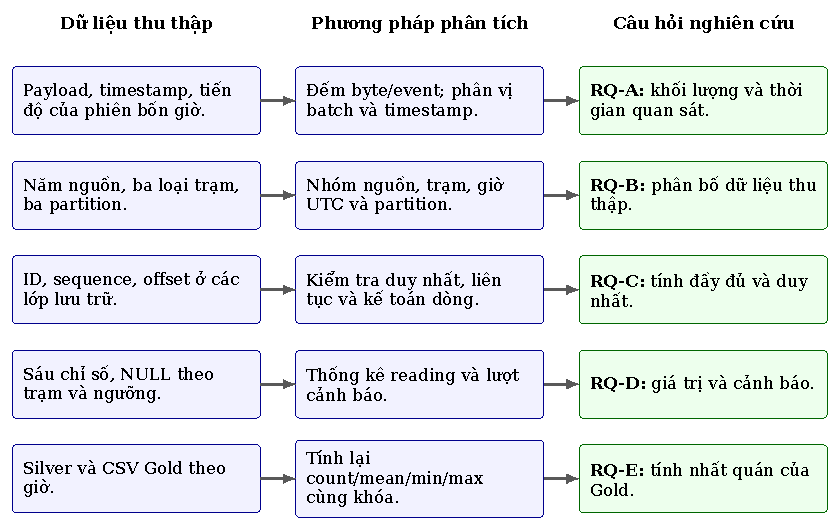
\includegraphics[width=0.95\linewidth]{figures/ch1-rq-map.pdf}
\endgroup
\caption{Mối liên hệ giữa dữ liệu thu thập, phương pháp phân tích và câu hỏi nghiên cứu.}
\label{fig:rq-motivation-map}
\end{figure}


Hình~\ref{fig:rq-motivation-map} nối từng đặc thù dữ liệu với một yêu cầu
thiết kế và một phép đánh giá. Nhờ đó, việc chọn Kafka, Spark hay mô hình
phân tầng lưu trữ được giải thích từ bài toán thay vì từ tên công nghệ.
RQ-A hiện có số đo tại một mức tải; RQ-B có phân bố partition và tài
nguyên nhưng chưa có đối chứng thay cấu hình; RQ-C/D có fixture bổ sung;
RQ-E có đối soát Gold và kiểm thử rerun ở fixture. Mỗi RQ cần có evidence tương ứng; một phép tải dài chỉ trả lời một phần
các câu hỏi về hiệu năng, chưa thay thế được phép đo bão hòa, phục hồi hay
kiểm tra chất lượng dữ liệu.

Với bộ RQ này, đề tài mang bản chất của một đánh giá hệ thống dữ liệu lớn:
các đặc trưng cốt lõi của Big Data đối với bài toán cảm biến --- Velocity
qua RQ-A/B/C và Veracity qua RQ-D --- được đưa về các phép đo cụ thể thay
vì mô tả định tính. Khả năng mở rộng được đánh giá ở phạm vi mà một
máy cho phép kiểm chứng (điều chỉnh mức song song, số nhân xử lý và số
nguồn phát); mở rộng sang nhiều máy (scale-out) không thuộc phạm vi này mà
chỉ hiện diện dưới dạng ranh giới kiến trúc, như Mục~\ref{sec:scope} sẽ
mô tả.

Việc hệ thống hỗ trợ sáu loại chỉ số môi trường là một lựa chọn có chủ đích
nhằm phân biệt một pipeline ``tình cờ chạy đúng'' với một kiến trúc xử lý
tổng quát: các trạm thật phát những tập con chỉ số khác nhau, nên một cơ chế
kiểm tra hay cảnh báo viết cứng cho một đại lượng duy nhất sẽ bộc lộ sai sót
ngay khi gặp các chỉ số có miền giá trị, đơn vị hoặc hướng ngưỡng khác.
RQ-D vì vậy được đặt trên ngữ nghĩa per-metric, trong đó bản tin thiếu một
số chỉ số là dữ liệu bình thường, chứ không phải trên giả định mọi bản tin
đều mang đủ sáu chỉ số.

\section{Phạm vi đề tài}
\label{sec:scope}

Báo cáo tập trung vào một bài toán đầy đủ nhưng có kiểm soát: xây dựng
và đánh giá một hệ thống streaming end-to-end chạy trọn trên một máy
Linux. Từ tầng tiếp nhận thiết bị qua MQTT, bộ đệm phân tán Kafka, tầng
xử lý Spark Structured Streaming, đến các lớp Bronze/Silver/Quarantine
trên Parquet cục bộ, PostgreSQL ở tầng phục vụ và lưu aggregate Gold, cùng
lớp truy vấn FastAPI/dashboard --- toàn bộ pipeline được đóng gói bằng
Docker Compose trong tổng giới hạn bộ nhớ khoảng 4,6~GiB cho chế độ
streaming; thành phần cụ thể, phiên bản và lý do lựa chọn từng công nghệ
được trình bày chi tiết ở Chương~\ref{chap:implementation}.

Về dữ liệu, hệ thống không dùng số đo từ cảm biến thật mà nhận tải tự
sinh từ các simulator. Lựa chọn này cho phép kiểm soát hai điều mà dữ
liệu thực tế hiếm khi cho phép cùng lúc: tải được phân bố theo nhiều
nguồn phát song song, và hành vi lỗi --- bản trùng, thiếu trường, giá trị
ngoài miền vật lý, event đến muộn --- được đặt trước bằng seed theo tỷ lệ
xác định. Seed và cấu hình hỗ trợ tái tạo workload, nhưng khả năng tái lập còn phụ
thuộc mã nguồn, trạng thái lưu trữ và lịch thực thi. Phiên tải dài tắt fault
injection; kiểm thử lỗi ở fixture được trình bày riêng, không suy ra từ
Quarantine rỗng của phiên sạch. Việc vận hành và quan sát tài nguyên
dùng script cùng \texttt{docker stats} thay cho một cụm giám sát riêng,
nhằm giữ ngân sách bộ nhớ cho chính pipeline.

Cùng nguyên tắc tiết chế tài nguyên, những yếu tố đòi hỏi hạ tầng nhiều
máy hoặc không thêm giá trị chứng minh cho đề tài được xếp ra ngoài
phạm vi và ghi nhận là hướng phát triển ở Chương~\ref{chap:conclusion}:
bảo mật TLS/SASL/ACL đầy đủ, sẵn sàng cao với nhiều broker Kafka có
replication và cụm Mosquitto, cụm Spark standalone nhiều worker, Delta
Lake/HDFS thay cho Parquet cục bộ, Kubernetes ở mức production, edge/fog
computing, và các kỹ thuật học tăng dần hay dự báo trên luồng.

Kiến trúc phân lớp tạo các điểm có thể mở rộng về sau --- tăng partition,
tăng tài nguyên Spark, thêm broker hoặc tách thành nhiều máy. Tuy nhiên,
mở rộng không chỉ là thay đổi cấu hình: nhân bản Bridge cần định danh
phiên riêng và cơ chế phân phối subscription phù hợp; cụm nhiều máy cần
lưu trữ dùng chung, replication và kiểm thử phục hồi tương ứng. Các phép
đo hiện tại đánh giá cấu hình một máy và chỉ ra các điểm cần đo tiếp,
chưa chứng minh điểm bão hòa hoặc khả năng mở rộng ngang của một cụm lớn.

Về trạng thái bằng chứng, một phép chạy dài đã được thực hiện trên máy mục
tiêu với năm nguồn phát đồng thời, thời lượng cấu hình 14.400 giây (manifest
nguồn ghi 14.405,067 giây quan sát). Phép chạy ghi nhận
50.760.004 bản ghi và 16.226.141.856 byte payload tại Bronze, đồng thời
pipeline đã drain Kafka và ổn định ở các query streaming. Đây là số đo thực
tế về khối lượng dữ liệu đi qua cấu hình một máy trong phiên quan sát; nó
được dùng để đối soát các ranh giới của pipeline, không dùng để suy ra năng
lực tổng quát của hệ thống. Chương~\ref{chap:results} tách số đo run dài,
fixture kiểm tra chức năng và kế hoạch kiểm chứng chưa chạy theo trạng thái
evidence tương ứng.

\section{Đóng góp của báo cáo}

Báo cáo đóng góp bốn điểm chính:

\begin{enumerate}
  \item \textbf{Một kiến trúc tham chiếu} cho hệ thống streaming IoT chạy
        trọn trên một máy với ngăn xếp hoàn toàn mã nguồn mở, trong đó các
        quyết định thiết kế đáng chú ý là tách bạch giao thức thiết bị khỏi
        giao thức xử lý, phân tầng Bronze/Silver/Quarantine trên Parquet
        cục bộ và aggregate Gold trong PostgreSQL,
        và đặt tính idempotency ở tầng phục vụ PostgreSQL thay vì tầng tệp
        (Chương~\ref{chap:implementation});
  \item \textbf{Một khung khái niệm veracity-aware event-time} làm hệ quy
        chiếu chung cho thiết kế và đánh giá. Khung gồm hai lớp tách bạch:
        các định nghĩa đã hiện thực trong baseline (bộ bốn trường
        định danh/thời gian, ba đại lượng độ trễ, vector veracity và cơ chế
        per-metric, các bất biến kế toán bản ghi) và các định nghĩa
        extension được khai báo rõ ở mức khái niệm, chưa triển khai và chưa
        có số đo (ngữ nghĩa watermark ở mức query, chính sách thích nghi
        FAST/CAUTIOUS, vòng đời công bố PROVISIONAL--FINAL--CORRECTED).
        Khung này được dùng làm ngôn ngữ chung cho báo cáo và không được
        trình bày như một framework thích nghi hoàn chỉnh;
  \item \textbf{Một phương pháp benchmark} gồm bảy kịch bản được thiết kế
        để chạy trên một máy và ánh xạ tường minh tới năm RQ, với metric
        được định nghĩa rõ ràng và điều kiện thí nghiệm được ghi đầy đủ,
        theo khuyến nghị về tính tái lập của các nghiên cứu thực hành
        benchmark và giám sát chất lượng dữ liệu stream-first gần
        đây~\cite{kafka_patterns_benchmark_2025, stream_daq_2024}. Phương
        pháp này đã được kiểm chứng một phần bằng phép chạy dài nhiều nguồn
        và đối soát khối lượng ở các ranh giới chính của pipeline;
  \item \textbf{Cách trình bày kết quả minh bạch}: Chương~\ref{chap:results}
        tách số đo run dài, fixture chức năng và kế hoạch chưa chạy.
        Benchmark công bố~\cite{shufflebench_2024, fault_recovery_stream_2024}
        và tài liệu Confluent~\cite{confluent_partition_count,
        confluent_optimize_clients} là cơ sở phương pháp thiết kế đối
        chứng; mỗi kết luận nêu phạm vi đo, evidence và giới hạn suy diễn.
\end{enumerate}

\section{Cấu trúc báo cáo}

Báo cáo gồm năm chương: Chương~\ref{chap:introduction} nêu bối cảnh,
mục tiêu và phạm vi; Chương~\ref{chap:background} trình bày cơ sở lý
thuyết; Chương~\ref{chap:implementation} mô tả kiến trúc và triển khai;
Chương~\ref{chap:results} trình bày phương pháp, kết quả đo và giới hạn
đánh giá; Chương~\ref{chap:conclusion} kết luận và đề xuất hướng phát triển.

\chapter{Cơ sở lý thuyết}
\label{chap:background}

Chương này trình bày nền tảng khái niệm và các công nghệ được sử dụng trong
báo cáo. Phần đầu tóm tắt đặc trưng Big Data và lý do dữ liệu cảm biến IoT
là một trường hợp tiêu biểu. Phần thứ hai xây dựng mô hình xử lý event-time
có nhận thức veracity (veracity-aware event-time) làm hệ quy chiếu cho toàn
bộ báo cáo. Phần thứ ba mô tả chức năng, cơ chế hoạt động và lý do lựa chọn
của từng thành phần công nghệ trong kiến trúc
Chương~\ref{chap:implementation}, theo chiều luồng dữ liệu: lớp thiết bị,
lớp đệm, lớp xử lý, lớp lưu trữ --- phục vụ và lớp điều phối batch. Phần
cuối tổng hợp các nghiên cứu liên quan --- gồm các thực hành benchmark cho
hệ thống event-streaming và các mô hình giám sát chất lượng dữ liệu
stream-first --- kèm bảng so sánh khoảng trống nghiên cứu.

Một quy ước đọc quan trọng xuyên suốt phần mô hình: mọi định nghĩa, metric
và bất biến được gắn một trong ba trạng thái bằng chứng --- \textbf{baseline
đã triển khai} (cơ chế tương ứng đang chạy trong
Chương~\ref{chap:implementation}), \textbf{có thể suy ra từ dữ liệu đã ghi}
(tính được từ log hoặc dòng đã lưu mà không cần thêm cơ chế mới), hoặc
\textbf{extension chưa triển khai} (định nghĩa ở mức khái niệm, chưa có mã
chạy và chưa có số đo). Các định nghĩa extension không được dùng để mô tả
hành vi của baseline.

\section{Tổng quan Big Data và đặc thù dữ liệu cảm biến IoT}
\label{sec:bigdata-overview}

Big Data thường được mô tả qua các đặc trưng Volume (khối lượng lớn),
Velocity (tốc độ sinh dữ liệu cao), Variety (đa dạng định dạng),
Veracity (độ tin cậy không đồng nhất) và Value (giá trị khai thác được).
Trong bối cảnh IoT sensor streaming, các đặc trưng thường bị ảnh hưởng mạnh
nhất là \textbf{Volume}, \textbf{Velocity} và \textbf{Veracity}: một cụm cảm
biến công nghiệp hoặc smart-city có thể sinh từ hàng triệu đến hàng tỷ event
mỗi ngày với
tần suất giây đến mili-giây, dung sai xử lý cuối cùng thường chỉ tính bằng
giây, và một tỷ lệ bản tin không hoàn hảo (muộn, trùng, ngoài ngưỡng vật
lý) luôn tồn tại trong luồng dữ liệu~\cite{iot_big_data_survey_2022}.

Các khảo sát về hệ thống phân tích IoT Big Data cũng chỉ ra rằng đường cong
tăng trưởng dữ liệu IoT kéo theo ba nhóm thách thức: (i) kiến trúc ingestion
chịu tải cao, (ii) lưu trữ có hỗ trợ ghi liên tục, và (iii) mô hình xử lý có
thể phục hồi sau sự cố~\cite{iot_big_data_survey_2022}. Đây chính là ba trụ
cột mà hệ thống được thiết kế trong báo cáo này nhắm tới; chiều Veracity
được bổ sung xuyên suốt như một trục thiết kế thay vì một bước hậu xử lý.

Khác với bài toán phân tích log/microservices truyền thống, dữ liệu cảm biến
có các tính chất khiến việc xử lý phải được thiết kế cẩn trọng ngay từ đầu:

\begin{itemize}
  \item \textbf{Tốc độ cao liên tục}: một dây chuyền với vài nghìn sensor,
        mỗi sensor đo 1--10 Hz, tạo ra hàng chục nghìn event/s;
  \item \textbf{Tính không hoàn hảo của timestamp}: event sinh ra tại cảm biến
        nhưng được nền tảng quan sát muộn hơn một lượng không hằng; event có
        thể đến sai thứ tự sinh, và chính timestamp cũng có thể lệch do clock
        cục bộ (xem Mục~\ref{subsec:lateness});
  \item \textbf{Trùng lặp}: do cơ chế retry hoặc idempotency yếu ở tầng gateway;
  \item \textbf{Giá trị giảm theo thời gian}: một cảnh báo nhiệt độ vượt ngưỡng
        gần như vô giá trị nếu đến tay người vận hành sau vài phút;
  \item \textbf{Tỷ lệ bản tin hỏng không đồng nhất}: noise, lỗi cảm biến,
        dropout kết nối tạo ra một tỷ lệ bản tin cần xử lý riêng, và tỷ lệ
        này khác nhau theo từng loại chỉ số đo.
\end{itemize}

Những tính chất này biến bài toán cảm biến IoT thành một use-case điển hình
của stream processing, nơi các khái niệm như event-time, idempotency và
fault tolerance trở thành yêu cầu cốt lõi
chứ không phải tùy chọn~\cite{iot_stream_latency_2021}.

\section{Mô hình hình thức: xử lý event-time có nhận thức veracity}
\label{sec:theory}

Mục này xây dựng mô hình khái niệm dùng chung cho toàn báo cáo: mọi cơ chế
trong Chương~\ref{chap:implementation} (validation per-metric, dedup,
quarantine, alert, batch aggregate) và mọi metric trong
Chương~\ref{chap:results} đều được ánh xạ về các định nghĩa ở đây. Các định
nghĩa không phụ thuộc công nghệ, nhưng mọi ví dụ cơ chế đều lấy từ pipeline
MQTT--Kafka--Spark--Parquet/PostgreSQL cụ thể của báo cáo.

Mô hình gồm hai lớp tách bạch. \textbf{Lớp baseline} là những gì đã được
hiện thực trong Chương~\ref{chap:implementation}: bộ bốn trường
định danh/thời gian, ba đại lượng độ trễ, vector veracity cùng cơ chế
per-metric, marker khử trùng và upsert idempotent ở PostgreSQL, và các bất
biến kế toán tương ứng. \textbf{Lớp extension} là những gì chỉ được định
nghĩa ở mức khái niệm, chưa triển khai và chưa có số đo: ngữ nghĩa
cửa sổ/watermark ở mức query, chính sách thích nghi FAST/CAUTIOUS và vòng
đời công bố PROVISIONAL--FINAL--CORRECTED. Lớp extension đóng vai trò khung
cho các giả thuyết cần đo (Mục~\ref{subsec:hypotheses}) và cho hướng phát
triển (Chương~\ref{chap:conclusion}); trong toàn bộ phần mô tả baseline,
báo cáo không dựa vào bất kỳ định nghĩa extension nào.

\subsection{Event, bản tin, row và vector chỉ số}
\label{subsec:event-tuple}

Trước hết, báo cáo chuẩn hóa bốn từ khóa và dùng nhất quán ở mọi chương:

\begin{itemize}
  \item \textbf{event} là đơn vị dữ liệu logic: một quan sát của một cảm
        biến tại một thời điểm, được định danh bởi \texttt{event\_id};
  \item \textbf{bản tin} (message) là biểu diễn của một event trên đường
        truyền --- một bản tin MQTT hoặc một bản ghi trong log Kafka;
  \item \textbf{row} là biểu diễn của một event sau khi được lưu trữ ---
        một dòng trong Parquet (Bronze, Silver, Quarantine) hoặc trong
        PostgreSQL;
  \item \textbf{reading} là một thành phần chỉ số của event --- một phần
        tử của vector đo --- và là đơn vị gốc của aggregate ở tầng Gold.
\end{itemize}

Sự phân biệt này quyết định ngữ nghĩa của từng cơ chế: dedup diễn ra trên
event (theo \texttt{event\_id}), quarantine diễn ra trên row, còn aggregate
và cảnh báo diễn ra trên reading. Một bản tin mang một event; một event được
lưu thành row; một event có thể sinh nhiều reading, mỗi chỉ số nó mang một
reading.

Với các định danh trên, mỗi event được mô hình hóa thành
\begin{equation}
  \begin{aligned}
    e &= \bigl(\mathit{event\_id},\ \mathit{sensor\_id},\ t^{e},\ t^{gw},\
         \mathbf{m}\bigr), \\
    \mathbf{m} &= (m_{\mathrm{temp}},\ m_{\mathrm{hum}},\ \ldots,\
         m_{\mathrm{light}}) \in \bigl(\mathbb{R} \cup \{\bot\}\bigr)^{6}.
  \end{aligned}
  \label{eq:event-tuple}
\end{equation}
theo đúng data contract khai báo trong Listing~\ref{lst:schema}: bốn trường
định danh và thời gian \textbf{bắt buộc} --- \texttt{event\_id},
\texttt{sensor\_id}, \texttt{event\_time} ($t^{e}$) và \texttt{ingest\_time}
($t^{gw}$) --- cùng vector đo $\mathbf{m}$ gồm sáu chỉ số môi trường (nhiệt
độ, độ ẩm, CO$_2$, áp suất, bụi mịn PM2.5, ánh sáng). Bốn trường này là điều
kiện cần để một row được chấp nhận vào Silver; thiếu hoặc sai một trong
chúng là lỗi định danh và được xử lý ở Mục~\ref{subsec:veracity}.

Mỗi thành phần $m_j$ nhận một giá trị số hoặc vắng mặt ($\bot$) tùy loại
trạm: trạm thời tiết phát nhiệt/ẩm/áp suất/ánh sáng, trạm chất lượng không
khí phát CO$_2$/PM2.5. \textbf{Chỉ số vắng mặt là dữ liệu bình thường,
không phải lỗi} (baseline đã triển khai): một row Silver hợp lệ chỉ mang tập
con chỉ số của trạm phát nó. Lỗi của từng chỉ số --- giá trị không parse
được số hoặc nằm ngoài miền vật lý --- được xử lý per-metric ở
Mục~\ref{subsec:veracity} và không làm mất row.

\subsection{Thời gian của event và ba đại lượng độ trễ}
\label{subsec:lateness}

Một event mang theo nhiều mốc thời gian; việc phân biệt chúng là nền tảng
của mọi định nghĩa độ trễ phía sau. Báo cáo dùng hệ ký hiệu thống nhất
trong Bảng~\ref{tab:time-taxonomy} ở mọi chương.

\begin{table}[H]
\centering
\caption{Phân loại các mốc thời gian của một event trong pipeline.}
\label{tab:time-taxonomy}
\begin{tabularx}{\textwidth}{c l X}
\toprule
\textbf{Ký hiệu} & \textbf{Tên} & \textbf{Điểm gắn và vai trò} \\
\midrule
$t^{e}$ & event time &
  Thời điểm hiện tượng vật lý xảy ra, do cảm biến gắn; là trục thời gian
  của mọi aggregate trong báo cáo (trường \texttt{event\_time}). \\
$t^{gw}$ & producer/gateway ingest time &
  Thời điểm producer đóng gói và phát bản tin; đại diện cho độ trễ phía
  ngoài nền tảng (trường \texttt{ingest\_time}). \\
$t^{k}$ & Kafka record timestamp &
  Timestamp gắn với bản ghi Kafka, được lưu ở Bronze dưới trường
  \texttt{kafka\_timestamp}. Baseline dùng \texttt{CreateTime} mặc định,
  do Kafka producer gắn; chỉ với cấu hình \texttt{LogAppendTime} mới
  biểu thị thời điểm broker append. Khoảng $t^{r}-t^{k}$ ở
  Chương~\ref{chap:results} chỉ là khoảng giữa hai timestamp đã lưu, không
  phải độ trễ của broker hay của cảm biến. \\
$t^{r}$ & platform receive time &
  Mốc xử lý micro-batch của query Q1, được gắn bằng
  \texttt{current\_timestamp()} và lưu thành trường provenance ở tầng
  Bronze (\texttt{received\_at\_utc}). \\
$t^{o}$ & publication time &
  Thời điểm dòng aggregate của một cửa sổ xuất hiện ở bảng Gold; tồn tại
  ở mức window, không phải mức event. \\
\bottomrule
\end{tabularx}
\end{table}

\begin{figure}[H]
\centering
\begin{tikzpicture}[
  font=\footnotesize,
  stage/.style={draw=blue!55!black, rounded corners=2pt, fill=blue!5,
    align=center, text width=2.85cm, minimum height=1.6cm, inner sep=4pt},
  link/.style={-{Latex[length=2mm]}, thick, draw=black!65},
  span/.style={{Latex[length=2mm]}-{Latex[length=2mm]}, thick, draw=blue!65!black}]
% Nhãn của các khoảng đặt dưới mũi tên (anchor=north) để không đè lên mũi tên.
\node[stage] (event) at (0,0) {\textbf{Cảm biến}\\$t^{e}$\\\texttt{event\_time}};
\node[stage] (producer) at (3.75,0) {\textbf{Producer}\\$t^{gw}$\\\texttt{ingest\_time}};
\node[stage] (kafka) at (7.5,0) {\textbf{Kafka}\\$t^{k}$\\\texttt{kafka\_timestamp}};
\node[stage] (spark) at (11.25,0) {\textbf{Spark Q1}\\$t^{r}$\\\texttt{received\_at\_utc}};
\draw[link] (event.east) -- (producer.west);
\draw[link] (producer.east) -- (kafka.west);
\draw[link] (kafka.east) -- (spark.west);
\foreach \x in {0,3.75,11.25} {\draw[dashed, black!35] (\x,-.85) -- (\x,-3.6);}
\draw[span] (0,-1.65) -- (3.75,-1.65);
\node[align=center, text width=3.4cm, anchor=north] at (1.875,-1.8)
  {$t^{gw}-t^{e}$\\đóng gói và trễ phía nguồn};
\draw[span] (3.75,-1.65) -- (11.25,-1.65);
\node[align=center, text width=6.6cm, anchor=north] at (7.5,-1.8)
  {$t^{r}-t^{gw}$\\truyền nhận, hàng đợi và chờ micro-batch};
\draw[span] (0,-3.6) -- (11.25,-3.6);
\node[align=center, text width=12.5cm, anchor=north] at (5.625,-3.75)
  {\textbf{Ingestion lateness:} $L_i=\max(0,t_i^{r}-t_i^{e})$; không đồng nhất với độ trễ mạng.};
\node[draw=black!35, fill=black!3, rounded corners=2pt,
  align=left, text width=13.4cm, inner sep=5pt, anchor=north] at (5.625,-4.7)
  {\textbf{Lưu ý về $t^{k}$:} baseline dùng Kafka \texttt{CreateTime} mặc định.
   Timestamp do producer gắn không phải thời điểm broker append.
   $t^{r}$ là timestamp xử lý của micro-batch Q1, không phải timestamp riêng cho từng gói mạng.};
\end{tikzpicture}
\caption{Các mốc thời gian và hai thành phần của ingestion lateness trong baseline. Vị trí các khối không theo tỷ lệ thời gian; phép so sánh giả định clock đã đồng bộ.}
\label{fig:event-time-path}
\end{figure}


Hình~\ref{fig:event-time-path} cho thấy cùng một bản ghi có nhiều mốc
thời gian với ý nghĩa khác nhau. Trong baseline, Kafka giữ timestamp
\texttt{CreateTime}~\cite{kafka_docs_4_3}; trường này không đo được riêng
thời điểm ghi log ở broker. Timestamp Q1 được gắn ở mức micro-batch, nên
lateness suy ra từ Bronze bao gồm cả thời gian chờ xử lý và cần được đọc
theo độ phân giải của trigger, thay vì xem là phép đo độ trễ mạng của từng
gói.

\textbf{Giả định clock.} Các so sánh timestamp trong báo cáo giả định clock
của cảm biến/gateway và của nền tảng được đồng bộ (ví dụ NTP) hoặc độ lệch
clock (skew) bị chặn trên bởi một hằng $\varepsilon$ nhỏ so với các ngưỡng
lateness được sử dụng. Nếu giả định này bị vi phạm, mọi ước lượng lateness
đều mang sai số hệ thống cỡ $\varepsilon$ và cần được nêu rõ khi phân tích.

Trên nền các mốc thời gian đó, \textbf{lateness quan sát được} (observed
lateness, hay \textit{ingestion lateness}) tại điểm nền tảng nhận là
\begin{equation}
  L_i \;=\; \max\bigl(0,\ t^{r}_i - t^{e}_i\bigr).
  \label{eq:observed-lateness}
\end{equation}
Đây là đại lượng mức event, tính được trực tiếp từ hai cột timestamp đã lưu
trong Bronze/Silver (\texttt{received\_at\_utc} và \texttt{event\_time}),
nên thuộc trạng thái \emph{có thể suy ra từ dữ liệu đã ghi}. Thành phần
$t^{r} - t^{e}$ không đồng nhất với network delay: $L_i$ là tổng hợp của
thời gian xử lý tại cảm biến, buffering tại gateway, retry, hàng đợi mạng
và cả sai lệch clock cục bộ (theo giả định clock nêu trên). Vì vậy một
chiến lược ``giảm latency mạng'' không nhất thiết làm giảm $L_i$ nếu nguyên
nhân nằm ở gateway hoặc clock.

Cần tách bạch ngay từ đầu ba đại lượng ``độ trễ'' khác cấp độ mà báo cáo
sử dụng, không gộp chung thành một con số:

\begin{itemize}
  \item \textbf{Ingestion lateness} $L_i$ --- mức event, tính từ timestamp
        của chính event theo Ct.~\ref{eq:observed-lateness}; đặc trưng cho
        khoảng cách giữa hiện tượng và lúc nền tảng thấy nó;
  \item \textbf{Kafka consumer lag} --- mức luồng, khoảng cách giữa offset
        cuối cùng của log partition (Log End Offset) và offset mà query
        đang đọc; đặc trưng cho tích lũy nguồn khi tốc độ vào vượt tốc độ
        xử lý;
  \item \textbf{Publication latency} --- mức window, khoảng thời gian từ
        khi cửa sổ kết thúc theo event time đến khi dòng aggregate tương
        ứng xuất hiện ở bảng Gold.
\end{itemize}
Ba đại lượng này được định nghĩa bằng công thức riêng trong
Chương~\ref{chap:results}; ở đây chỉ cần cố định tên gọi và cấp độ của
chúng.

Một event $e_j$ gọi là \textbf{đến sai thứ tự} (out-of-order) nếu tồn tại
$e_i$ với $t^{e}_i < t^{e}_j$ nhưng $t^{r}_i > t^{r}_j$. Out-of-order là hệ
quả trực tiếp của lateness không đồng đều giữa các event, và là lý do các
phép tính aggregate đặt trên trục $t^{e}$ thay vì trục thời gian đến.

Việc một event có ``đến sau watermark'' hay không là một vị từ (predicate)
khác, phụ thuộc thêm vào tiến độ đọc của query tại thời điểm event đến;
vị từ này thuộc extension chưa triển khai và được định nghĩa riêng ở
Mục~\ref{subsec:watermark}. Không suy ra nó trực tiếp từ $L_i$.

\subsection{Vector veracity và cơ chế baseline}
\label{subsec:veracity}

Đặc trưng Veracity của Big Data được báo cáo cụ thể hóa thành một vector chất
lượng 5 chiều, mỗi chiều là một câu hỏi có thể kiểm tra trên từng bản ghi
hoặc từng luồng:
\begin{equation}
  \mathcal{V}(e) = \bigl(C_{\mathrm{comp}},\ C_{\mathrm{val}},\
  C_{\mathrm{uniq}},\ C_{\mathrm{time}},\ C_{\mathrm{cons}}\bigr).
  \label{eq:veracity-vector}
\end{equation}
Bảng~\ref{tab:veracity-mapping} nêu định nghĩa từng chiều và ánh xạ tới cơ
chế baseline trong Chương~\ref{chap:implementation}; toàn bộ năm cơ chế
trong bảng thuộc trạng thái \textbf{baseline đã triển khai}.

\begin{table}[H]
\centering
\caption{Năm chiều veracity và ánh xạ tới cơ chế baseline.}
\label{tab:veracity-mapping}
\small
\begin{tabularx}{\textwidth}{l X X}
\toprule
\textbf{Chiều} & \textbf{Câu hỏi} & \textbf{Cơ chế baseline tương ứng} \\
\midrule
Completeness & Row có đủ các trường định danh/thời gian bắt buộc không? &
  Q2a/Q2b kiểm tra bốn trường bắt buộc: \texttt{event\_id},
  \texttt{sensor\_id} khác rỗng; \texttt{event\_time},
  \texttt{ingest\_time} parse được, chuẩn UTC. Vi phạm $\rightarrow$ cả
  row vào Quarantine kèm \texttt{error\_reason}; thiếu
  \texttt{event\_id} dùng key dự phòng topic--partition--offset. \\
Validity & Giá trị từng chỉ số có parse được số và nằm trong miền vật lý
  hợp lệ không? &
  Kiểm tra per-metric theo bảng cấu hình (bounds inclusive): chỉ số
  không parse được hoặc ngoài miền vật lý bị \textbf{che lọc (mask)
  thành NULL} trong Silver, reason \texttt{non\_numeric:<m>} /
  \texttt{value\_out\_of\_bounds:<m>} ghi vào \texttt{metric\_issues};
  row vẫn giữ. Chỉ số vắng (station subset) không phải lỗi; vượt ngưỡng
  cảnh báo vẫn hợp lệ. \\
Uniqueness & \texttt{event\_id} có xuất hiện nhiều lần không? &
  Khử trùng ở tầng phục vụ, không trong state streaming: Q3 ghi marker
  \texttt{processed\_events} (khóa chính \texttt{event\_id}) idempotent;
  replay tăng \texttt{duplicate\_count}; re-send cùng \texttt{event\_id}
  với vector chỉ số khác được phát hiện. Batch Gold chọn một row theo
  \texttt{ROW\_NUMBER} với thứ tự xác định cho mỗi \texttt{event\_id}. \\
Timeliness & Event đến muộn bao nhiêu? &
  Cờ \texttt{is\_late} trong Silver đánh khi $t^{r} - t^{e}$ vượt
  \texttt{LATE\_THRESHOLD\_S} (mặc định 60 giây); event muộn hợp lệ
  không bị quarantine. Vị từ post-watermark là extension
  (Mục~\ref{subsec:watermark}). \\
Consistency & Các mốc thời gian có nhất quán không? &
  Baseline bảo đảm ở mức parse: cả hai mốc \texttt{event\_time} và
  \texttt{ingest\_time} bắt buộc parse được, chuẩn hóa UTC khi ghi
  Silver; ngoài mức parse, baseline chưa có kiểm tra chéo sâu hơn giữa
  hai mốc. \\
\bottomrule
\end{tabularx}
\end{table}

Bảng trên cho thấy ba mức ngữ nghĩa phân biệt rõ trong cơ chế baseline:

\begin{itemize}
  \item \textbf{Mức row}: chỉ lỗi định danh/thời gian đưa cả row vào
        Quarantine; đây là trường hợp duy nhất một row bị loại khỏi Silver;
  \item \textbf{Mức metric}: lỗi của một chỉ số chỉ làm mất giá trị chỉ số
        đó (mask NULL kèm reason), không ảnh hưởng các chỉ số khác của cùng
        row và không đưa row vào Quarantine;
  \item \textbf{Mức event}: bản trùng vẫn hiện diện trong Silver (Silver cố
        ý cho phép lặp để không mất dữ liệu ở tầng tệp) nhưng chỉ được công
        bố một lần ở tầng phục vụ, qua marker \texttt{processed\_events} và
        dedup của batch.
\end{itemize}

\begin{figure}[H]
\centering
\begingroup
\setstretch{1}
\begin{tikzpicture}[
  font=\footnotesize,
  block/.style={draw=blue!55!black, rounded corners=2pt, fill=blue!5,
    align=center, text width=5.1cm, minimum height=1.15cm, inner sep=5pt},
  reject/.style={block, text width=3.65cm, fill=orange!9, draw=orange!65!black},
  output/.style={block, text width=4.85cm, fill=green!7, draw=green!40!black},
  link/.style={-{Latex[length=2mm]}, thick, draw=black!65}]
% Vị trí tương đối: mũi tên bám cạnh hộp, hai hộp cuối cùng có chung mép trên.
\node[block, text width=8.0cm] (bronze) at (0,0)
  {\textbf{Bronze}\\Mỗi bản ghi Kafka được lưu nguyên payload cùng provenance.};
\node[block, below=0.9cm of bronze] (row)
  {\textbf{Mức row: kiểm tra định danh/thời gian}\\Bốn trường bắt buộc hợp lệ?};
\node[reject, below=1.7cm of row, xshift=-3.9cm] (quarantine)
  {\textbf{Quarantine}\\Giữ cả row lỗi cùng \texttt{error\_reason}.};
\node[block, below=1.7cm of row, xshift=3.2cm] (metric)
  {\textbf{Mức metric: chỉ số}\\Lỗi $\rightarrow$ NULL + \texttt{metric\_issues}.\\Chỉ số vắng không phải lỗi.};
\node[block, fill=green!7, draw=green!40!black, below=1.0cm of metric] (silver)
  {\textbf{Silver}\\Giữ row hợp lệ, các chỉ số còn dùng được và cờ \texttt{is\_late}; bản trùng vẫn được lưu.};
\node[output, below=1.5cm of silver, xshift=-2.85cm] (serving)
  {\textbf{Mức event: phục vụ Q3}\\Marker \texttt{processed\_events}; upsert giá trị mới nhất và cảnh báo theo khoá.};
\node[output, below=1.5cm of silver, xshift=2.85cm] (gold)
  {\textbf{Mức event: batch Gold}\\Chọn một row/\texttt{event\_id} theo thứ tự xác định; tách reading; tổng hợp theo giờ.};
\coordinate (splitrow) at ([yshift=-0.85cm]row.south);
\draw[link] (bronze) -- (row);
\draw[link] (row.south) -- (splitrow) -- node[above]{không} (splitrow -| quarantine.north) -- (quarantine.north);
\draw[link] (row.east) -- (row.east -| metric.north) -- node[right]{có} (metric.north);
\draw[link] (metric) -- (silver);
\draw[link] (silver.south) -- ++(0,-0.75) -| (serving.north);
\draw[link] (silver.south) -- ++(0,-0.75) -| (gold.north);
\node[draw=black!35, fill=black!3, rounded corners=2pt,
  text width=13.3cm, align=center, inner sep=5pt, anchor=north]
  at ([yshift=-0.7cm]silver.south |- serving.south)
  {\textbf{Kế toán tầng tệp sau drain, trước khử trùng:}
   $N_{\mathrm{Bronze}}=N_{\mathrm{Silver}}+N_{\mathrm{Quarantine}}$.\\
   Không cộng lại số bản trùng ở tầng phục vụ vào đẳng thức này.};
\end{tikzpicture}
\endgroup
\caption{Ba mức xử lý chất lượng dữ liệu của baseline: row quyết định nhánh lưu trữ, metric quyết định giá trị giữ lại và event quyết định tính duy nhất khi phục vụ hoặc tổng hợp.}
\label{fig:validation-levels}
\end{figure}


Hình~\ref{fig:validation-levels} làm rõ vì sao ``dữ liệu lỗi'' không đồng
nghĩa với việc bỏ cả bản tin. Một row có định danh hợp lệ vẫn vào Silver
nếu chỉ một metric lỗi; giá trị metric đó được che lọc và giữ lý do để
hậu kiểm. Cũng tại Silver, bản trùng được giữ để bảo toàn lịch sử tiếp
nhận. Batch Gold chỉ chọn một bản theo \texttt{event\_id}, ưu tiên
\texttt{received\_at\_utc} mới nhất, rồi \texttt{kafka\_partition} và
\texttt{kafka\_offset} giảm dần; sau đó chỉ các reading khác NULL mới góp
vào thống kê. Quy tắc chọn xác định này khác với việc chọn tùy ý một bản
trong nhóm trùng.

\subsection{Metric chất lượng rolling và trạng thái bằng chứng}
\label{subsec:rolling-metrics}

Để biến veracity vector thành đại lượng vận hành, báo cáo định nghĩa sáu
metric rolling, tính trên cửa sổ trượt (hoặc theo epoch chính sách trong
Mục~\ref{subsec:policy} khi extension đó được triển khai). Mỗi metric được
gắn trạng thái bằng chứng theo quy ước của chương:

\begin{enumerate}
  \item \textbf{p95 lateness} [\emph{có thể suy ra từ dữ liệu đã ghi}]:
        phân vị 95 của $L_i$ (Ct.~\ref{eq:observed-lateness}) trên các
        event nhận trong khoảng rolling; đặc trưng cho đuôi của phân phối
        đến muộn. Tính được từ hai cột timestamp đã lưu trong
        Bronze/Silver;
  \item \textbf{Late-event ratio} $\rho_{\mathrm{late}}$ [\emph{baseline:
        cờ đã ghi; ratio có thể suy ra}]: tỷ lệ event có $L_i$ vượt một
        ngưỡng $\ell$ chọn trước trên tổng event nhận trong khoảng.
        Baseline dùng $\ell$ = \texttt{LATE\_THRESHOLD\_S} (60 giây),
        trùng với ngưỡng của cờ \texttt{is\_late} đã ghi trong Silver.
        Ngưỡng đặt trên $L_i$ là một chỉ báo vận hành, không đồng nhất với
        vị từ post-watermark (Mục~\ref{subsec:watermark});
  \item \textbf{Duplicate ratio} $\rho_{\mathrm{dup}}$ [\emph{có thể suy ra
        từ dữ liệu đã ghi}]: trong tập row Silver được chọn, tỷ lệ bản
        thừa so với số \texttt{event\_id} phân biệt, tức
        $(N_{\mathrm{Silver}}-N_{\mathrm{distinct\ event\_id}})
        /N_{\mathrm{Silver}}$ với cùng phạm vi quan sát. Bộ đếm
        \texttt{duplicate\_count} ở Q3 còn bao gồm replay do micro-batch
        chạy lại, nên được báo riêng và không tự động bằng tỷ lệ trùng
        sinh ra ở nguồn;
  \item \textbf{Invalid/quarantine ratio} $\rho_{\mathrm{inv}}$
        [\emph{có thể suy ra từ dữ liệu đã ghi}]: tỷ lệ row bị tách sang
        Quarantine vì lỗi định danh; riêng tỷ lệ chỉ số bị che lọc (NULL
        kèm reason trong \texttt{metric\_issues}) được thống kê
        per-metric;
  \item \textbf{Watermark lag} [\emph{extension chưa triển khai}]: hiệu
        giữa đồng hồ vật lý hiện tại và watermark của query đang chạy;
        lag tăng kéo dài là dấu hiệu pipeline không theo kịp input rate.
        Ở baseline chưa khai báo watermark, backlog được quan sát bằng
        Kafka consumer lag (Mục~\ref{subsec:lateness}); consumer lag theo
        offset không phải watermark lag theo thời gian;
  \item \textbf{Policy transition count} [\emph{extension chưa triển
        khai}]: số lần chuyển trạng thái FAST $\leftrightarrow$ CAUTIOUS
        trong một khoảng quan sát; chỉ có ý nghĩa khi chính sách ở
        Mục~\ref{subsec:policy} được triển khai.
\end{enumerate}

Ba tỷ lệ (late-event, duplicate, invalid/quarantine) là ước lượng mẫu; sai số
thống kê của chúng tuân theo quy luật
lấy mẫu thông thường và cần được nêu kèm khoảng tin cậy khi dùng làm ngưỡng
quyết định --- đây là nội dung của giả thuyết H2
(Mục~\ref{subsec:hypotheses}).

\subsection{Extension event-time: cửa sổ và watermark (chưa triển khai)}
\label{subsec:watermark}

Toàn bộ mục này thuộc \textbf{lớp extension chưa triển khai}: các query
streaming của baseline không khai báo watermark (được chứng minh ở cuối
mục), nên mọi vị từ và ngữ nghĩa dưới đây mô tả hành vi của một query
giả định có khai báo watermark, dùng làm khung cho extension và cho các giả
thuyết cần đo.

\textbf{Cửa sổ event-time.} Với độ dài cửa sổ $w$ và mốc căn chỉnh $t_0$,
cửa sổ thứ $m$ là nửa khoảng
\begin{equation}
  W_m = [\,t_0 + m w,\ t_0 + (m+1) w\,)
  \label{eq:window-def}
\end{equation}
và event $e_i$ được gán vào $W_m$ khi $t^{e}_i \in W_m$ (tumbling window;
mọi window trong báo cáo thuộc loại này). Khái niệm cửa sổ trên trục
$t^{e}$ không thuộc riêng extension: batch Gold của baseline cũng aggregate
theo cửa sổ giờ trên \texttt{event\_time}. Điểm chỉ có ở extension là
watermark --- biến trạng thái quyết định ``cửa sổ khi nào được coi là đã
nhận đủ''.

\textbf{Watermark.} Với một query $Q$ đọc luồng event và ngưỡng trễ
$\theta \geq 0$, watermark được mô hình hóa cho một nguồn event-time
tại thời điểm $t$ là
\begin{equation}
  W_Q(t) \;=\; M_Q(t) - \theta,
  \qquad
  M_Q(t) = \max_{e \in E_Q(t)} t^{e}
  \label{eq:watermark-def}
\end{equation}
trong đó $E_Q(t)$ là tập event mà $Q$ đã đọc tính đến $t$. Vì $M_Q(t)$ không
giảm theo $t$, watermark có tính đơn điệu:
\begin{equation}
  t_1 \leq t_2 \;\Longrightarrow\; W_Q(t_1) \leq W_Q(t_2).
  \label{eq:watermark-mono}
\end{equation}
Đây là mô hình khái niệm; Spark cập nhật watermark theo tiến độ
micro-batch, và query nhiều nguồn còn có chính sách ghép watermark riêng.
Vì vậy không xem Ct.~\ref{eq:watermark-def} là một phép cập nhật tức thời
cho từng record trong engine.

\textbf{Lateness so với watermark.} Cho $a_i$ là thời điểm query $Q$ xử lý
record chứa $e_i$ (ở Bronze, xấp xỉ $t^{r}_i$). Event $e_i$ gọi là
\textbf{đến sau watermark} (post-watermark) của $Q$ khi tại thời điểm đến,
watermark đã vượt qua event time của nó, tức $t^{e}_i \leq W_Q(a_i)$.
Đây là vị từ khác với observed lateness $L_i$
(Ct.~\ref{eq:observed-lateness}): $L_i$ chỉ phụ thuộc hai timestamp của
chính event, còn vị từ post-watermark phụ thuộc cả tiến độ đọc $M_Q$ của
query. Hai vị từ chỉ tương quan, không tương đương: với $\theta = 10$ phút,
một event có $L_i = 12$ phút vẫn có thể đến trước watermark nếu luồng đến
chậm ($M_Q$ còn thấp), và ngược lại một event có $L_i = 6$ phút vẫn có thể
đến sau watermark nếu các event khác đã đưa $M_Q$ vượt qua event time của
nó. Do đó không được suy ``$L_i > \theta$ nên event post-watermark'' như
một kết luận tất yếu.

\textbf{Ngữ nghĩa.} Watermark là một tuyên bố tiến độ ở mức query/window: ``$Q$
xem như đã nhận đủ mọi event có $t^{e} \leq W_Q(t)$''. Nó phục vụ hai việc:
(i) giới hạn state (ví dụ state dedup chỉ cần giữ trong horizon $\theta$);
(ii) hỗ trợ \textit{finalization} --- quyết định khi nào một cửa sổ được chốt
kết quả trong chế độ streaming. Watermark là cơ chế đánh đổi
correctness--latency--cost kinh điển của xử lý dữ liệu unbounded: $\theta$ lớn
giữ được nhiều event muộn nhưng state lớn và kết quả chốt muộn; $\theta$ nhỏ
ngược lại~\cite{dataflow_model_2015}.

Hai hiểu lầm cần loại bỏ ngay từ đầu:
\begin{itemize}
  \item Watermark không phải ``thùng rác'': event đến sau watermark
        (post-watermark) \emph{không} tự động bị xoá hay tự động vào
        quarantine. Hành vi cụ thể phụ thuộc loại query và output mode của
        nó. Với query chỉ chiếu và ghi bản ghi thô, không có operator
        stateful, khai báo watermark không tự tạo một bộ lọc xoá bản ghi.
        Với operator aggregation hoặc dedup có state, bản quá muộn có
        thể bị loại theo ngữ nghĩa operator. Spark bảo đảm giữ dữ liệu
        nằm trong ngưỡng trễ khai báo, nhưng dữ liệu ngoài ngưỡng có thể
        được xử lý hoặc bị loại, không có bảo đảm một chiều ngược lại.
        Khi cửa
        sổ đã được chốt và state của nó đã được giải phóng, event
        post-watermark không thể cập nhật aggregate đó nữa --- chế độ
        \texttt{append} không phát hành thêm dòng cho cửa sổ đã chốt, và
        chế độ \texttt{update} cũng vậy vì state đã bị dọn. Chế độ
        \texttt{complete} giữ toàn bộ state aggregate và công bố toàn bộ
        bảng kết quả mỗi trigger, nên không dùng watermark để dọn state
        cũ; baseline không dùng chế độ này~\cite{spark_docs_4_2}.
  \item Watermark không phải độ trễ mạng và không phải SLA: nó là biến trạng
        thái của query, tiến theo dữ liệu thực tế đã đọc, không theo đồng hồ
        vật lý.
\end{itemize}

Trong Structured Streaming, watermark được khai báo ở mức query bằng
\texttt{withWatermark} và gắn với một cột event-time~\cite{spark_docs_4_2,
structured_streaming_sigmod_2018}. Ranh giới với cài đặt phải nêu rõ:
\textbf{không query nào trong baseline khai báo watermark}. Dữ liệu đến
muộn được xử lý qua cờ \texttt{is\_late} theo ngưỡng
\texttt{LATE\_THRESHOLD\_S} và qua tính lại batch; các query streaming
Q1--Q3 là phép chiếu, lọc và \texttt{foreachBatch} stateless nên không có
state aggregate cần chốt. Do đó $\theta$ hiện chỉ là tham số của mô hình và
của extension thích nghi (Mục~\ref{subsec:policy}), chưa phải cấu hình đang
chạy.

\subsection{Extension vận hành: chính sách thích nghi và vòng đời công bố (chưa triển khai)}
\label{subsec:policy}
\label{subsec:lifecycle}

Toàn bộ mục này cũng thuộc \textbf{lớp extension chưa triển khai}; các cơ
chế được mô tả để định nghĩa giả thuyết H4 và để chỉ ra seam nâng cấp
trong kiến trúc hiện có, không mô tả hành vi đang chạy.

\textbf{Chính sách hai trạng thái (đề xuất).} Trên nền metric rolling, báo
cáo đề xuất một chính sách hai trạng thái điều chỉnh hành vi xử lý theo
chất lượng quan sát được. Đây là thiết kế \textit{policy epoch / feedback}:
cứ sau mỗi epoch (ví dụ một cụm batch), controller đọc vector metric, so
với ngưỡng và quyết định trạng thái cho epoch kế tiếp. Chính sách thay đổi
tham số của query (ngưỡng $\theta$, horizon dedup) giữa các epoch ---
\emph{không} phải cơ chế watermark per-record native của Spark; mỗi query tại
một thời điểm vẫn chạy với một watermark cố định theo ngữ nghĩa
Mục~\ref{subsec:watermark}.

Hai trạng thái:
\begin{itemize}
  \item \textbf{FAST}: chất lượng quan sát tốt (luồng đến đúng giờ, ít trùng,
        ít lỗi). Nước đi của trạng thái này: $\theta$ nhỏ (khởi điểm từ giá
        trị đo được của p95 lateness), state dedup gọn, kết quả chốt sớm.
  \item \textbf{CAUTIOUS}: chất lượng quan sát xấu đi (p95 lateness hoặc
        $\rho_{\mathrm{late}}$ tăng). Nới $\theta$ và horizon dedup để giữ
        thêm event muộn, đánh đổi bằng state lớn hơn và publication chậm hơn.
\end{itemize}

Ký hiệu $\phi$ là metric điều khiển (ví dụ p95 lateness chuẩn hóa), $u$ là
ngưỡng lên và $d$ là ngưỡng xuống ($d < u$). Chuyển trạng thái tức thời theo
một batch duy nhất dễ gây dao động (flapping) khi metric nhiễu quanh ngưỡng,
nên báo cáo dùng \textbf{hysteresis theo số batch liên tiếp}: trạng thái chỉ
đổi khi điều kiện được giữ liên tiếp trong $n$ epoch:
\begin{equation}
  \text{FAST} \xrightarrow{\ \phi \geq u\ \text{liên tiếp}\ n\ \text{epoch}\ }
  \text{CAUTIOUS}
  \qquad
  \text{CAUTIOUS} \xrightarrow{\ \phi \leq d\ \text{liên tiếp}\ n\ \text{epoch}\ }
  \text{FAST}.
  \label{eq:hysteresis}
\end{equation}

\textbf{Hard safety bounds.} Để policy không thể tự nới lỏng hệ thống ra ngoài
miền an toàn, tồn tại các bound cứng không bị policy vượt qua, độc lập với
trạng thái: (i) $\theta \leq \theta_{\max}$ (chặn trên của watermark);
(ii) horizon dedup và thời gian giữ state có chặn trên theo dung lượng;
(iii) mọi record vẫn phải được kế toán theo bất biến I1
(Mục~\ref{subsec:invariants}) --- policy chỉ thay đổi cách phân loại đúng hạn
so với muộn, không thay đổi tổng số record phải giải trình.

Điểm can thiệp (seam) của extension trong kiến trúc Chương~\ref{chap:implementation}
là nơi controller đọc metric từ nguồn quan sát đã có (Mục quan sát vận hành
phía dưới) và khởi động lại query với tham số mới --- tức là tác động vào khâu
khởi tạo query, không thay đổi mô hình thực thi (Bronze/Silver vẫn streaming,
Gold vẫn batch). Lợi ích và chi phí của chính sách này là đối tượng của giả
thuyết H4 (Mục~\ref{subsec:hypotheses}).

\textbf{Giao thức liên tục giữa các epoch (đề xuất, chưa kiểm chứng).} Vì
watermark được tính lại từ tiến độ đọc của từng query
(Ct.~\ref{eq:watermark-def}), một query khởi động mới --- kể cả khi chỉ đổi
$\theta$ --- không tự động kế thừa watermark của query cũ: nếu state không
được khôi phục, watermark sẽ bắt đầu từ mức thấp và có nguy cơ nhảy lùi so
với mốc frontier (giá trị watermark cuối cùng) mà pipeline đã đạt được. Để
bất biến I2 (Mục~\ref{subsec:invariants}) giữ đúng xuyên các epoch, báo cáo
đề xuất giao thức tối thiểu sau:
\begin{itemize}
  \item trước khi dừng query cũ, controller chốt lại frontier watermark cuối
        cùng cùng với checkpoint/offset của query, và ưu tiên tái sử dụng cùng
        \texttt{checkpointLocation} để Spark khôi phục state (kể cả watermark)
        thay vì khởi động hoàn toàn từ đầu;
  \item frontier hiệu dụng không bao giờ bị hạ: watermark của epoch mới phải
        khởi động từ $\max(\text{frontier cũ},\ \text{watermark mới tính
        được})$;
  \item các cửa sổ biên --- window mà việc chốt kết quả phụ thuộc $\theta$ cũ
        hay mới --- phải được đối chiếu/replay bằng pass batch trước khi được
        coi là FINAL;
  \item mọi chuyển epoch được ghi audit (epoch, $\theta$ cũ/mới, frontier
        trước/sau, số cửa sổ biên) và gắn với metric policy transition count;
        hiện tượng watermark lùi được coi là vi phạm I2 cần cảnh báo.
\end{itemize}
Đây là thiết kế đề xuất, chưa được triển khai và chưa được kiểm chứng; tính
đơn điệu xuyên epoch là điều kiện phải được bảo đảm và audit, không phải hành
vi tự động của query restart.

Liên quan trực tiếp đến chính sách trên là câu hỏi về \emph{địa vị} của kết
quả được công bố sớm --- nội dung của vòng đời công bố.
\textbf{Vòng đời (đề xuất, chưa triển khai).} Khi kết quả window được công bố
trước khi
cửa sổ nhận đủ mọi event (điều bắt buộc nếu muốn có số sớm), mỗi aggregate cần
một vòng đời trạng thái rõ ràng. Gọi \textbf{logical key} của một aggregate là
\begin{equation}
  K = (W_m,\ \mathit{dimensions})
  \label{eq:logical-key}
\end{equation}
gồm cửa sổ $W_m$ (Ct.~\ref{eq:window-def}) và bộ chiều nhóm (baseline:
\texttt{sensor\_id} $\times$ chỉ số đo). Ba trạng thái:

\begin{itemize}
  \item \textbf{PROVISIONAL}: aggregate được công bố khi watermark chưa vượt
        qua $W_m$; giá trị có thể còn thay đổi.
  \item \textbf{FINAL}: watermark đã vượt qua $W_m$ cộng thêm một khoảng ân
        hạn (grace); aggregate được chốt và là nguồn cho truy vấn chuẩn.
  \item \textbf{CORRECTED}: sau FINAL, vẫn có thể xuất hiện event rất muộn
        hoặc bản chỉnh sửa (ví dụ sau khi đối chiếu với batch pass); aggregate
        được tính lại và ghi đè bản FINAL cũ, kèm tham chiếu tới phiên bản
        trước.
\end{itemize}

Hai yêu cầu đi kèm: (i) \textbf{reconciliation} --- một job batch định kỳ đối
chiếu các cửa sổ đã FINAL với dữ liệu đầy đủ hơn và phát hành CORRECTED khi
chênh lệch vượt ngưỡng; (ii) \textbf{idempotency} --- việc ghi lại cùng một
logical key $K$ phải là merge/upsert theo $K$, không phải append mù, để chạy
lại không tạo bản sao. Đây là tinh thần ``batch layer sửa lỗi cho speed
layer'' của kiến trúc Lambda~\cite{lambda_adsb_2023} áp dụng ở mức window.

\textbf{Khoảng cách với baseline.} Cài đặt hiện tại chỉ hiện thực một góc của
vòng đời này: aggregate Gold được tính bằng batch theo giờ, tính lại từ toàn
bộ dữ liệu Silver của cửa sổ và ghi bằng \emph{upsert idempotent theo khóa}
(cảm biến, giờ, chỉ số) cho các khóa mà lần chạy tính ra --- chạy lại cùng
cửa sổ trên cùng dữ liệu nguồn cho kết quả xác định, không cộng dồn;
câu lệnh upsert không xoá các
dòng nằm ngoài tập khóa của lần chạy. Các query baseline không khai báo
watermark, nên không có khái niệm ``cửa sổ đã chốt'' theo
Mục~\ref{subsec:watermark}. Phần còn thiếu so với vòng đời đề xuất là: kênh
công bố sớm PROVISIONAL từ streaming (serving realtime hiện dựa vào bảng
\texttt{sensor\_latest} theo event, không phải aggregate window), cột trạng
thái và cơ chế phát hành chênh lệch CORRECTED. Việc bổ sung đầy đủ lifecycle
là một phần của hướng phát triển (Chương~\ref{chap:conclusion}).

\subsection{Bất biến kế toán và giả thuyết kiểm chứng}
\label{subsec:invariants}
\label{subsec:hypotheses}

Một pipeline veracity-aware đúng phải giữ các bất biến sau, bất kể policy ở
trạng thái nào. Mỗi bất biến được gắn trạng thái (baseline đã triển khai
hoặc extension chưa triển khai) và, khi có, cơ chế cụ thể trong
Chương~\ref{chap:implementation}.

\begin{description}
  \item[\textbf{I1.}] \textbf{Kế toán row ở tầng tệp (baseline).} Với cùng
        tập bản ghi nguồn và sau khi Q2a/Q2b đã drain, mỗi row Bronze rơi
        vào đúng một trong hai nhánh: Silver hoặc Quarantine. Không khử
        trùng ở bước này, nên số row phải bảo toàn:
        \begin{equation}
          N_{\mathrm{Bronze}} \;=\; N_{\mathrm{Silver}}
          + N_{\mathrm{Quarantine}}.
          \label{eq:accounting}
        \end{equation}
        Cơ chế: Q2a/Q2b dùng hai predicate bổ trợ, độc quyền; lỗi
        định danh/thời gian giữ nguyên row ở Quarantine kèm lý do. Lỗi
        metric và bản trùng vẫn nằm trong Silver, nên không được cộng
        một lần nữa như row bị loại. Khi đối chiếu tầng phục vụ, dùng
        kế toán riêng cho số lượt thử ghi: lượt xử lý mới và lượt
        replay/trùng; \texttt{duplicate\_count} có thể tăng khi cùng
        micro-batch chạy lại dù số row Parquet không tăng. Đẳng thức
        trên cũng không thay thế phép đối chiếu số bản tin được phát với
        số bản ghi đã tới Kafka/Bronze.
  \item[\textbf{I2.}] \textbf{Đơn điệu watermark (extension).} Trong phạm vi một
        query \emph{có khai báo watermark}, $W_Q(t)$ không giảm theo $t$
        (Ct.~\ref{eq:watermark-mono}); đây là ngữ nghĩa của Spark Structured
        Streaming~\cite{spark_docs_4_2}. Vì baseline không khai báo watermark
        ở bất kỳ query nào, bất biến này hiện không áp dụng cho query nào
        đang chạy. Xuyên các epoch policy (restart query với $\theta$ mới),
        tính đơn điệu \emph{không} tự động được bảo đảm: query mới tính lại
        watermark từ tiến độ đọc của chính nó trừ khi state được khôi phục.
        Điều kiện để bất biến giữ đúng là giao thức liên tục ở
        Mục~\ref{subsec:policy} (không hạ frontier hiệu dụng, khôi phục/ghép
        frontier cũ); điều kiện này là đề xuất cần kiểm chứng và phải được
        audit, chưa phải hành vi đã đo của Spark.
  \item[\textbf{I3.}] \textbf{Khử trùng dựa trên marker bền vững (baseline).}
        Nhận diện bản trùng không nằm trong state streaming của Spark mà
        trong bảng marker \texttt{processed\_events} của PostgreSQL: mỗi
        \texttt{event\_id} đã được áp vào bảng phục vụ có đúng một dòng;
        replay tăng \texttt{duplicate\_count} thay vì tạo dòng mới; re-send
        cùng \texttt{event\_id} với vector chỉ số khác được phát hiện qua
        truy vấn payload-conflict. Giới hạn cần nêu rõ:
        \texttt{processed\_events} \emph{không phải bounded state} --- bảng
        này tăng theo số \texttt{event\_id} đã xử lý và không bị chặn bởi
        horizon thời gian; vai trò của nó là marker kế toán/khử trùng bền
        vững (sống sót qua restart, hậu kiểm được), không phải state dedup
        có chặn trên. Việc giới hạn state dedup theo horizon watermark là
        phương án của extension thích nghi (Mục~\ref{subsec:policy}); batch
        Gold loại trùng trên một khoảng giờ hữu hạn nên tập key của nó hữu
        hạn theo thiết kế.
  \item[\textbf{I4.}] \textbf{Khóa công bố duy nhất (baseline).} Mọi aggregate ở
        Gold có đúng một logical key $K$ (Ct.~\ref{eq:logical-key}): khóa
        (cảm biến, giờ, chỉ số). Cơ chế hiện tại:
        \texttt{gold.sensor\_hourly} ghi bằng \emph{upsert idempotent theo
        khóa} đối với các khóa xuất hiện trong lần chạy batch --- chạy lại
        cùng cửa sổ không cộng dồn. Nói chính xác: batch tính lại
        aggregate từ toàn bộ dữ liệu Silver của cửa sổ nên mọi khóa có dữ
        liệu trong cửa sổ đều được ghi đè giá trị mới, nhưng câu lệnh
        \emph{không xoá} các dòng nằm ngoài tập khóa của lần chạy; vì vậy
        đây là upsert idempotent theo batch, không phải full-replace toàn
        bảng.
  \item[\textbf{I5.}] \textbf{Hội tụ chỉnh sửa (extension).} Dưới giả định (a)
        lateness bị chặn trên bởi $\theta + $ grace và (b) dữ liệu nguồn cho
        phép replay đầy đủ, tồn tại thời điểm hữu hạn mà sau đó mọi aggregate
        CORRECTED bằng aggregate tính trên dữ liệu đầy đủ; số lần chỉnh sửa
        của mỗi window là hữu hạn. Cơ chế đề xuất: reconciliation batch
        trong Mục~\ref{subsec:lifecycle}~\cite{dataflow_model_2015}.
\end{description}

Trong năm bất biến trên, I1, I3 và I4 thuộc baseline đang chạy và được unit
test phủ trực tiếp (Chương~\ref{chap:implementation}); I2 và I5 là điều
kiện của extension, chưa có cơ chế chạy kèm.

Bên cạnh các bất biến \emph{phải} giữ, mô hình còn sinh ra các giả thuyết
\emph{có thể} kiểm chứng. Báo cáo đặt bốn giả thuyết
\textbf{chưa được kiểm chứng}
trong phạm vi báo cáo này; chúng xác định các phép đo bổ sung cần thực
hiện trên hệ thống:

\begin{itemize}
  \item[H1.] Tăng allowed lateness (watermark bound $\theta$) làm tăng tỷ lệ
        event muộn được giữ lại, nhưng đồng thời tăng kích thước state và làm
        chậm thời điểm công bố kết quả window. Cần đo bộ ba (retention, state,
        publication delay) theo $\theta$.
  \item[H2.] Các bộ đếm chất lượng (quarantine ratio, duplicate ratio, late
        ratio) bám đúng profile lỗi được inject trong sai số lấy mẫu: với
        $N$ record, sai lệch kỳ vọng giảm theo $1/\sqrt{N}$. Kiểm chứng bằng
        cách so sánh tỷ lệ quan sát với tỷ lệ inject đã biết trước.
  \item[H3.] Reconciliation (tính lại cửa sổ từ dữ liệu đầy đủ hơn) làm giảm
        sai lệch của aggregate so với giá trị đầy đủ tại các cửa sổ đủ cũ;
        mức giảm phụ thuộc vào tỷ lệ event đến muộn sau thời điểm FINAL.
  \item[H4.] Chính sách thích nghi FAST/CAUTIOUS chỉ có lợi khi sự thay đổi
        của workload/chất lượng kéo dài hơn chi phí chuyển policy (restart
        query, làm ấm lại state); nếu shift ngắn hơn chi phí chuyển, policy cố
        định với $\theta$ chọn đúng có thể tốt hơn. Kiểm chứng đòi hỏi
        ablation: (i) fixed vs adaptive, (ii) adaptive có hysteresis vs không
        có hysteresis.
\end{itemize}

Các giả thuyết H1--H4 chưa có bộ thực nghiệm đủ để xác nhận. Chúng được
giữ làm kế hoạch đánh giá extension; H2 cũng cần so sánh tỷ lệ inject với
tỷ lệ quan sát trên nhiều cỡ mẫu. Điều này không phủ nhận những số đo
baseline đã có trong Chương~\ref{chap:results}: phép chạy dài
ngày 02/10/2026 là số đo runtime; fixture chức năng có
evidence riêng. Các đối chứng chưa chạy được giữ dưới dạng kế hoạch
kiểm chứng, chưa phải kết quả thực nghiệm.

\section{Các công nghệ chính}

\subsection{Apache Kafka --- distributed ingestion layer}

Apache Kafka là nền tảng phân tán lưu trữ và truyền tải event theo mô hình
append-only log~\cite{kafka_docs_4_3}. Trong báo cáo, Kafka đóng vai trò
buffer giữa lớp sinh dữ liệu (sensor simulator) và lớp xử lý (Spark), cho
phép hai bên vận hành độc lập về tốc độ.

Hai khái niệm then chốt trong Kafka là \textbf{topic} và \textbf{partition}.
Một topic được phân chia thành nhiều partition; mỗi partition là một log
có thứ tự, là đơn vị nhỏ nhất của song song~\cite{confluent_partition_count}.
Số partition quyết định mức song song tối đa của consumer trong cùng một
consumer group, đồng thời ảnh hưởng trực tiếp đến throughput producer.

Từ Kafka 4.0, chế độ ZooKeeper đã bị loại bỏ; dòng Kafka 4.x vận hành
bằng KRaft~\cite{kafka_docs_4_3}. Vì vậy Docker
image chính thức \texttt{apache/kafka:4.3.1} có thể khởi động một broker
chỉ với biến môi trường mà không cần triển khai ZooKeeper riêng.

Kafka hỗ trợ các lựa chọn về ngữ nghĩa giao hàng và xử lý, gồm
\textit{at-most-once}, \textit{at-least-once} và các cơ chế
\textit{exactly-once} trong phạm vi giao dịch Kafka. Producer idempotent
tránh bản trùng do retry trong phiên producer; transaction còn cần phối
hợp dữ liệu đầu ra và consumer offset khi xây dựng xử lý exactly-once
giữa các topic Kafka~\cite{kafka_docs_4_3}. Các cấu hình này không tự tạo
giao dịch nguyên tử giữa MQTT, Parquet và PostgreSQL.
Trong kiến trúc của báo cáo, Kafka producer không phải thiết bị cảm biến
(chúng chỉ nói MQTT) mà là Bridge: Bridge dùng \texttt{acks=all} và chỉ xác
nhận lại với broker MQTT sau khi Kafka giao thành công. Cơ chế này cho
phép phát lại trong giới hạn phiên bền, dung lượng hàng đợi và dữ liệu
được broker giữ; phần trùng lặp do phát lại được khử ở hạ lưu theo định
danh sự kiện. Với một broker và replication factor bằng 1, \texttt{acks=all}
không tạo thêm bản sao hay khả năng chịu hỏng đĩa.

\begin{figure}[H]
\centering
\begingroup
\setstretch{1}
\begin{tikzpicture}[
  font=\footnotesize,
  block/.style={draw=blue!55!black, rounded corners=2pt, fill=blue!5,
    align=center, text width=3.15cm, minimum height=.85cm, inner sep=4pt},
  task/.style={block, fill=orange!7, draw=orange!55!black},
  slot/.style={block, fill=green!7, draw=green!40!black},
  link/.style={-{Latex[length=2mm]}, thick, draw=black!65}]
\node[block, minimum height=2.9cm] (keys) at (0,-1.15)
  {\textbf{Bản tin MQTT}\\key: \texttt{sensor\_id}\\A, B, C, A, \ldots\\\emph{Tên key minh hoạ}};
\node[block, minimum height=2.0cm] (producer) at (4.6,-1.15)
  {\textbf{Bridge / Producer}\\Gán partition theo key và cấu hình partitioner.};
\node[block] (p0) at (9.2,0) {Partition P0\\log có thứ tự riêng};
\node[block] (p1) at (9.2,-1.15) {Partition P1\\log có thứ tự riêng};
\node[block] (p2) at (9.2,-2.3) {Partition P2\\log có thứ tự riêng};
\node[font=\footnotesize\bfseries] at (9.2,.9) {Topic \texttt{sensor\_raw}: 3 partition};
\draw[link] (keys) -- (producer);
\draw[link] (producer.east) -- (7,-1.15) |- (p0.west);
\draw[link] (producer.east) -- (p1.west);
\draw[link] (7,-1.15) |- (p2.west);
\node[align=center, text width=12.8cm] at (4.6,-3.6)
  {\textbf{Đọc nguồn Kafka của Q1 trong một micro-batch}\\Tác vụ bám partition; số partition không chứng minh các key được chia đều.};
\node[task] (t0) at (0,-4.8) {Task đọc P0};
\node[task] (t1) at (4.6,-4.8) {Task đọc P1};
\node[task] (t2) at (9.2,-4.8) {Task đọc P2};
\node[slot] (s0) at (2.3,-6.6) {Slot thực thi 1\\một task đang chạy};
\node[slot] (s1) at (6.9,-6.6) {Slot thực thi 2\\một task đang chạy};
\draw[link] (t0.south) -- (s0.north);
\draw[link] (t1.south) -- (s1.north west);
\draw[link, dashed] (t2.south) -- node[pos=.5, right=3pt, inner sep=2pt, align=left]{chờ slot\\trống} (s1.north east);
\node[draw=black!35, fill=black!3, rounded corners=2pt,
  text width=13.1cm, align=center, inner sep=5pt] at (4.6,-8.15)
  {\texttt{local[2]} cung cấp tối đa hai slot task cho SparkSession.
   Bốn query streaming dùng chung tài nguyên này. Tăng partition không tự tăng CPU, RAM hay tốc độ ghi sink.};
\end{tikzpicture}
\endgroup
\caption{Phân hoạch Kafka và giới hạn đồng thời của Spark trong cấu hình một máy. Gán key và thứ tự các task là sơ đồ minh hoạ, không phải phân bố partition hoặc lịch thực thi đã đo.}
\label{fig:partition-concurrency}
\end{figure}


Hình~\ref{fig:partition-concurrency} tách hai giới hạn thường bị nhầm:
partition tạo cơ hội đọc song song, còn số slot Spark quyết định số task
đồng thời có thể thực thi. Một key ổn định thường đi vào cùng partition
theo partitioner khi số partition không đổi, nhưng không bảo đảm các key
được chia đều. Spark Structured Streaming đọc Kafka theo tác vụ của
micro-batch; không áp dụng máy móc quy tắc consumer group để suy ra số
query có thể chạy. Trong baseline, topic có ba partition và bốn query
dùng chung SparkSession \texttt{local[2]}, nên phép đo mở rộng cần theo
dõi thêm CPU, backlog, thời lượng trigger và sink.

\subsection{Apache Spark Structured Streaming --- stream processor}

Spark Structured Streaming là một engine xử lý stream dựa trên Spark SQL
và bộ API DataFrame cùng Dataset~\cite{structured_streaming_sigmod_2018}. Khác với
các API streaming cũ (DStream) hoạt động trên RDD, Structured Streaming
mô hình hóa dữ liệu unbounded như một bảng liên tục được mở rộng theo
event-time~\cite{spark_docs_4_2}.

Hệ thống mặc định vận hành theo cơ chế \textbf{micro-batch}: dữ liệu
đến được đệm trong một khoảng trigger interval, sau đó được xử lý như
một mini-batch~\cite{spark_docs_4_2}. Nhờ vậy, cùng một mã nguồn có
thể chạy cho cả batch lẫn streaming, đơn giản hóa đáng kể quá trình phát
triển.

Engine cung cấp sẵn các primitive event-time: \textbf{event-time window}
(phép tính theo \texttt{event\_time} thay vì thời điểm nhận), \textbf{watermark}
(tiến độ ở mức query giới hạn trễ cho phép của dữ liệu muộn, hỗ trợ giới hạn
state và finalization) và \textbf{streaming deduplication} (loại trùng theo
khóa, có thể giới hạn bởi watermark)~\cite{spark_docs_4_2}; định nghĩa hình
thức của các primitive này nằm ở Mục~\ref{subsec:watermark}. Cách baseline
sử dụng cần nêu rõ để tránh suy diễn quá mức: bốn query streaming (Q1--Q3)
là phép chiếu, lọc và \texttt{foreachBatch} \emph{stateless} --- không thực
hiện aggregate, không khai báo watermark, không dùng dedup state của engine;
duy nhất batch Gold thực hiện aggregate theo event-time, tính theo giờ trên
\texttt{event\_time} sau khi loại trùng theo \texttt{event\_id}. Các
primitive nêu trên là nền tảng mà extension event-time
(Mục~\ref{subsec:watermark}, Mục~\ref{subsec:policy}) dự kiến dùng khi được
triển khai.

Về mặt fault tolerance, Structured Streaming ghi lại trạng thái của
mỗi query vào một \textit{checkpoint location}. Khi driver restart,
query được khôi phục từ checkpoint và tiếp tục từ vị trí batch cuối
cùng~\cite{spark_docs_4_2}. File sink Parquet của Structured Streaming
có metadata commit theo batch và bảo đảm \textbf{exactly-once} trong phạm
vi query với nguồn có thể replay và checkpoint được giữ. Đây không phải
giao dịch ACID đa bảng của bản thân định dạng Parquet, và cũng không phải
giao dịch nguyên tử giữa các query hoặc sink~\cite{spark_docs_4_2,
structured_streaming_sigmod_2018}. Với sink ngoài qua
\texttt{foreachBatch}, bảo đảm này không tự có --- nếu micro-batch được chạy
lại, sink bên ngoài có thể nhận bản trùng --- và phụ thuộc tính idempotent
của từng sink. Baseline của báo cáo chọn hướng idempotency ở tầng phục vụ:
sink PostgreSQL đạt được bằng staging + upsert theo khóa chính (như đã nêu
ở mục lưu trữ phía dưới), không thêm tầng table format, và báo cáo
\emph{không tuyên bố} exactly-once xuyên toàn pipeline; mục tiêu đã hiện
thực là replay an toàn và không cộng dồn ở các bảng phục vụ.

\subsection{Lưu trữ: các lớp Parquet cục bộ và PostgreSQL}

Apache Parquet là định dạng lưu trữ cột (columnar) nén, tối ưu cho truy
vấn phân tích và là định dạng đầu ra mặc định của Spark Structured
Streaming~\cite{spark_docs_4_2}. Trong bản triển khai một máy của báo cáo,
ba lớp dữ liệu Bronze/Silver/Quarantine được ghi dưới dạng Parquet trên một
thư mục bind mount cục bộ (gắn vào container tại \texttt{/data/bigdata}),
thay vì đặt trên một hệ thống tệp phân tán như HDFS~\cite{hdfs_docs_3_5}
hay một open table format như Delta Lake~\cite{delta_lake_docs}. Lựa chọn
này giữ ngân sách tài nguyên thấp cho bản demo mà vẫn bảo toàn \emph{hình
dạng} kiến trúc medallion: dữ liệu thô (Bronze), dữ liệu đã làm sạch
(Silver), dữ liệu lỗi bị cách ly (Quarantine) và dữ liệu tổng hợp (Gold)
vẫn tách biệt theo đúng vai trò.

Điểm đánh đổi so với Delta Lake/HDFS là: Parquet cục bộ không cung cấp
transaction log, ACID đa người ghi, time travel hay replication ở tầng tệp.
Vì vậy tính idempotency (chạy lại không tạo bản sao, không cộng dồn kết
quả) được đảm bảo ở \emph{tầng phục vụ} bằng các ràng buộc khóa chính và
câu lệnh upsert của PostgreSQL, cùng batch Gold tính lại từ Silver rồi ghi
bằng upsert theo khóa (chi tiết ngay dưới). Việc nâng cấp sang Delta
Lake trên HDFS hoặc object storage --- để có ACID/time travel ở tầng tệp và
replication chịu lỗi --- được ghi nhận là hướng phát triển
(Chương~\ref{chap:conclusion}) chứ không thuộc phạm vi bản một máy.

Một vấn đề thường gặp với streaming là \textit{small-file problem}: mỗi
micro-batch có thể tạo một tệp Parquet rất nhỏ, làm giảm hiệu năng truy
vấn về sau. Trong bản triển khai này, việc đọc luồng tệp (file stream) từ
Bronze/Silver được giới hạn số tệp mỗi trigger để kiểm soát áp lực, và tác
vụ gom tệp/retention có thể được đặt lịch bằng cron khi dữ liệu đủ lớn.

Nếu Parquet gánh phần lưu trữ phân tích thì phần phục vụ truy vấn dùng một
hệ quản trị quan hệ. PostgreSQL là hệ quản trị cơ sở dữ liệu quan hệ mã
nguồn mở, được dùng
trong báo cáo làm nơi lưu dữ liệu phục vụ truy vấn real-time (giá trị mới
nhất theo cảm biến, bản tin cảnh báo) và aggregate Gold theo giờ. Một
instance PostgreSQL duy nhất với database \texttt{app} phục vụ cả hai vai trò
này; các bảng dữ liệu và bảng aggregate nằm trong các schema tách biệt.

Vai trò then chốt của PostgreSQL trong kiến trúc này là gánh phần
\emph{idempotency} mà Parquet cục bộ không cung cấp: bảng giá trị mới nhất
dùng khóa chính theo cảm biến và chỉ ghi đè khi event mới hơn (so sánh
hàng giá trị có thứ tự xác định); bảng cảnh báo dùng khóa chính kép
(event, quy tắc) với xung đột thì bỏ qua; bảng marker
\texttt{processed\_events} ghi nhận mọi event đã áp vào bảng phục vụ
(replay tăng bộ đếm trùng thay vì tạo dòng mới); bảng Gold dùng
\emph{upsert idempotent theo khóa} (cảm biến, giờ, chỉ số) đối với các khóa
mà batch tính ra trong cửa sổ, nên chạy lại cùng cửa sổ không cộng dồn ---
và, như đã nêu, câu lệnh không xoá các dòng nằm ngoài tập khóa của lần chạy.
Các câu lệnh upsert này là nguồn sự thật duy nhất (single source of truth)
cho ngữ nghĩa chống trùng và được kiểm thử độc lập bằng SQLite trong bộ
unit test (Chương~\ref{chap:implementation}). Transaction giữa việc ghi
Parquet và việc ghi PostgreSQL không nguyên tử xuyên hai sink; bản ghi tạm
(staging) còn sót lại do crash giữa hai bước sẽ được dọn ở đầu lần ghi kế
tiếp, và việc đối chiếu dựa vào chính các upsert idempotent nêu trên.

\subsection{MQTT và Bridge --- lớp tiếp nhận thiết bị}

MQTT là giao thức nhắn tin nhẹ theo mô hình publish/subscribe, được thiết
kế cho thiết bị IoT có tài nguyên hạn chế và mạng không ổn định, với ba
mức chất lượng dịch vụ (QoS 0/1/2)~\cite{mqtt_v311_spec}. Trong báo cáo,
broker Mosquitto tiếp nhận bản tin QoS 1 từ các simulator cảm biến. Việc
dùng MQTT ở biên thiết bị --- thay vì cho Spark đọc thẳng từ một giao thức
khác --- tách bạch \emph{giao thức thiết bị} khỏi \emph{giao thức xử lý}
(Kafka): engine xử lý không cần biết MQTT tồn tại, nên việc thay broker,
thêm bảo mật hay đổi nguồn phát đều không lan sang tầng xử lý.

Giữa MQTT và Kafka là một \textbf{Bridge} Python đóng vai trò lớp dịch giao
thức độc lập. Bridge đăng ký MQTT với phiên bền (persistent session) và cơ
chế xác nhận thủ công (manual ACK): nó chỉ gửi ACK cho broker \emph{sau khi}
Kafka báo đã ghi bản tin thành công (\texttt{acks=all}). Nếu Bridge ngừng
giữa lúc produce và ACK, broker sẽ phát lại bản tin chưa được xác nhận khi
kết nối lại; chừng nào broker còn giữ được bản tin trong phiên bền (cấu hình demo đặt
\texttt{persistence false}, nên phiên và hàng đợi chỉ nằm trong bộ nhớ broker
và mất khi broker khởi động lại), đoạn
tiếp nhận đạt ngữ nghĩa at-least-once và phần trùng lặp do phát lại được
khử ở hạ lưu theo định danh sự kiện. Khi hàng đợi trong bộ nhớ của Bridge
đầy, bản tin bị bỏ qua mà \emph{không} ACK để broker giữ lại và phát lại;
tuy nhiên, hàng đợi của phiên bền phía broker có giới hạn cấu hình
(\texttt{max\_queued\_messages} của Mosquitto, đặt 5000 trong bản demo), nên
khi tắc nghẽn kéo dài broker cuối cùng buộc phải bỏ bản tin mới đến --- cửa
sổ mất dữ liệu này được ghi nhận tường minh trong mã nguồn Bridge, vì thế
bảo đảm at-least-once chỉ có giá trị trong giới hạn hàng đợi phía broker
chứ không tuyệt đối. Lớp Bridge cũng là ranh giới mở rộng ngang ở tầng tiếp
nhận: về nguyên tắc, khi tải tăng có thể nhân bản nhiều instance Bridge,
mỗi instance cần một định danh phiên MQTT và một định danh producer Kafka
riêng để các luồng ghi không can thiệp lẫn nhau. Bản triển khai hiện tại
vẫn dùng một định danh cố định cho cả hai phía và chưa có cấu hình định
danh theo instance, nên nhân bản Bridge mới là hướng mở rộng được ghi nhận
ở Chương~\ref{chap:conclusion} chứ chưa phải capability đã có sẵn. Ngoài
định danh, các instance phải có cơ chế chia subscription phù hợp (ví dụ
chia topic hoặc shared subscription); các subscriber độc lập cùng đăng
ký toàn bộ topic sẽ nhận nhiều bản sao, không tự chia tải.

\begin{figure}[H]
\centering
\begin{tikzpicture}[
  font=\footnotesize,
  actor/.style={draw=blue!55!black, rounded corners=2pt, fill=blue!5,
    align=center, text width=3.0cm, minimum height=1.2cm, inner sep=4pt},
  message/.style={-{Latex[length=2mm]}, thick, draw=blue!65!black},
  ack/.style={-{Latex[length=2mm]}, thick, draw=green!45!black},
  mlabel/.style={above, align=center, inner sep=2pt}]
% Nhãn đặt trong khoảng giữa hai đường sống, không đè lên đường nét đứt.
\node[actor] at (0,0) {Simulator\\publisher MQTT};
\node[actor] at (3.8,0) {Mosquitto\\broker MQTT};
\node[actor] at (7.6,0) {Bridge subscriber\\+ producer};
\node[actor] at (11.4,0) {Kafka\\broker};
\foreach \x in {0,3.8,7.6,11.4} {\draw[dashed, black!40] (\x,-.6) -- (\x,-8.3);}
\draw[message] (0,-1.3) -- node[mlabel]{1. PUBLISH QoS 1} (3.8,-1.3);
\draw[ack] (3.8,-2.6) -- node[mlabel]{2. PUBACK\\cho publisher} (0,-2.6);
\draw[message] (3.8,-3.9) -- node[mlabel]{3. PUBLISH QoS 1} (7.6,-3.9);
\draw[message] (7.6,-5.2) -- node[mlabel]{4. produce,\\\texttt{acks=all}} (11.4,-5.2);
\draw[ack] (11.4,-6.5) -- node[mlabel]{5. delivery\\callback: OK} (7.6,-6.5);
\draw[ack] (7.6,-7.8) -- node[mlabel]{6. PUBACK thủ công} (3.8,-7.8);
\node[draw=orange!60!black, fill=orange!7, rounded corners=2pt,
  text width=13.3cm, align=left, inner sep=5pt] at (5.7,-9.7)
  {\textbf{Khoảng có thể phát lại:} Bridge ngừng sau khi Kafka nhận bản tin nhưng trước bước 6.
   Mosquitto giữ bản chưa ACK trong phiên bền và có thể phát lại khi Bridge kết nối lại;
   định danh \texttt{event\_id} giúp hạ lưu nhận diện bản trùng.};
\end{tikzpicture}
\caption{Hai vòng xác nhận MQTT QoS 1 độc lập và điểm ACK thủ công của Bridge. Đây là một trình tự minh hoạ; PUBACK cho publisher không xác nhận rằng Kafka hoặc PostgreSQL đã ghi thành công.}
\label{fig:mqtt-ack-boundary}
\end{figure}


Hình~\ref{fig:mqtt-ack-boundary} phân biệt PUBACK mà simulator nhận từ
Mosquitto với PUBACK Bridge gửi về Mosquitto. Hai phiên QoS 1 này độc lập:
broker có thể xác nhận publisher trước khi Bridge hoặc Kafka hoàn tất
xử lý~\cite{mqtt_v311_spec}. Thứ tự bắt buộc trong Bridge là delivery
Kafka thành công trước ACK thủ công, còn các bước xác nhận publisher và
chuyển bản tin cho subscriber có thể xen kẽ. Vì thế số bản tin simulator
được ACK không tự chứng minh số bản ghi đã tới Bronze; cần đối chiếu log
phát, log delivery và row lưu trữ theo cùng phạm vi.

\subsection{Điều phối batch và quan sát vận hành bằng script}

Tác vụ tổng hợp Gold theo giờ có điểm bắt đầu/kết thúc rõ ràng và chạy lặp
lại theo lịch. Trong bản một máy, việc này được giao cho script wrapper
\texttt{run-batch-hourly} được cron của host khởi theo chu kỳ. Script trước
hết dùng một khóa loại trừ dựa trên thư mục kèm ghi PID: từ chối lần chạy
mới nếu batch trước còn chạy và tự dọn khóa cũ nếu process đó đã chết. Sau
đó script xác định cửa sổ giờ UTC vừa kết thúc, chờ một khoảng nới lỏng cấu
hình được (\texttt{BATCH\_GRACE\_S}) để các event sát ranh giới kịp nằm
trong Silver, rồi gọi đúng chương trình batch cho cửa sổ đó --- song song
với chế độ live đang chạy, không dừng nguồn phát và không đợi pipeline
drain. Ngược lại, đường batch một lượt (\texttt{run-mode.sh batch}) dành
cho tái xử lý thủ công mới dừng simulator và Bridge, chờ Spark tiêu hết
backlog Kafka, rồi mới dừng stream job và chạy batch. Một nền tảng điều phối
tác vụ đầy đủ (Airflow hoặc tương đương) chỉ trở nên cần thiết khi số lượng
DAG, phụ thuộc giữa tác vụ và nhu cầu quan sát lịch sử chạy tăng lên; lựa
chọn đó được ghi nhận là hướng phát triển ở Chương~\ref{chap:conclusion}.

Cùng triết lý ``dùng nguồn số liệu sẵn có thay vì dựng thêm hệ thống'' là
quan sát vận hành. Trong bản triển khai một máy, hệ thống không dựng một cụm
giám sát riêng kiểu Prometheus, Grafana hay JMX Exporter (để giữ ngân sách
bộ nhớ), mà thu các luồng bằng chứng độc lập với nhau: (i) tiến độ truy vấn
của Spark Structured Streaming qua query progress API --- ứng dụng ghi mỗi
trigger một dòng JSONL kèm \texttt{numInputRows}, thời lượng trigger và
offset đầu/cuối của nguồn Kafka~\cite{spark_docs_4_2}; (ii) các bộ đếm phía
PostgreSQL/API: số event đã áp vào bảng phục vụ, số bản trùng lặp, số cảnh
báo và thời điểm xử lý gần nhất; (iii) thống kê tài nguyên container qua
\texttt{docker stats} cùng RAM và dung lượng trống của host; và (iv) trạng
thái backlog: end offset của Kafka, số tệp Parquet ở từng tầng và số dòng
các bảng PostgreSQL. Một script thu thập lấy mẫu các nguồn (iii)--(iv) theo
chu kỳ và ghi mỗi mẫu thành một dòng \texttt{resource-report.jsonl} trên
bind mount. Các luồng này là bằng chứng cho người vận hành và nguyên liệu
phân tích benchmark (Chương~\ref{chap:results}); chúng không phải kênh dữ
liệu của dashboard --- dashboard đọc trực tiếp các endpoint ứng dụng của
backend.

Cách tiếp cận này đánh đổi khả năng cảnh báo và trực quan hóa tập trung của
một bộ Prometheus cùng Grafana lấy sự gọn nhẹ phù hợp bản demo; việc chuyển
sang một cụm
quan sát đầy đủ (Prometheus pull model, JMX Exporter cho JVM của Kafka và
Spark,
Grafana alerting) được ghi nhận là hướng phát triển
(Chương~\ref{chap:conclusion}) và không làm thay đổi các metric cần thu thập,
vì các đại lượng này đều trích được từ query progress API, thống kê
container và các bộ đếm PostgreSQL. Nguồn
metric này cũng là đầu vào mà chính sách thích nghi đề xuất ở
Mục~\ref{subsec:policy} đọc vào mỗi epoch.

\section{Các nghiên cứu liên quan}
\label{sec:related-work}

Ba khảo sát tổng quan cung cấp bối cảnh cho toàn chương:
\cite{iot_big_data_survey_2022} vẽ bức tranh thách thức
ingestion--storage--processing của IoT Big Data (đã dùng ở
Mục~\ref{sec:bigdata-overview}),
\cite{stream_processing_evolution_2024} tổng hợp sự tiến hóa của stream
processing theo bốn trục state management, fault tolerance, elasticity và
load management, còn \cite{iot_stream_latency_2021} phân loại các loại
latency trong truy vấn IoT stream --- cơ sở để
Chương~\ref{chap:results} phân biệt các loại trễ thay vì gộp chung một con
số. Phần còn lại của mục này so sánh các công trình trực tiếp liên quan đến
mô hình và phương pháp của báo cáo theo năm nhóm: kiến trúc IoT và testbed
thực nghiệm, nền tảng event-time, thích nghi và chỉnh sửa, thực hành
benchmark, và giám sát chất lượng stream-first.

\subsection{Kiến trúc IoT và testbed thực nghiệm}

Khattach và cộng sự~\cite{iot_end_to_end_2025} nghiên cứu kiến trúc đầu cuối
cho phân tích IoT và bảo trì dự đoán, kết hợp Kafka, Spark, InfluxDB cùng
pipeline học máy và quan sát vận hành. Điểm liên quan là cách tách tiếp
nhận, ETL, lưu trữ và khai thác dữ liệu. Mục tiêu của công trình còn bao
gồm dự đoán hỏng hóc và quản lý mô hình; đề tài này tập trung vào data
contract đa chỉ số, kế toán bản ghi và kiểm tra Gold. Vì vậy, kiến trúc
tương đồng không đồng nghĩa cùng bài toán kiểm chứng, và chất lượng dự
đoán của công trình không được dùng đánh giá nền tảng này.

Testbed Czech Post của \v{S}tufi và Ba\v{c}i\'{c}~\cite{iot_testbed_2021} khảo sát luồng
IoT dựa trên MQTT trong nền tảng phân tích có khả năng mở rộng, dùng ứng
dụng Java đa luồng để tạo tải và công bố cấu hình cùng kết quả thử nghiệm.
Broker MQTT được thử trên một nút ảo, trong khi kiến trúc tổng thể có
nhiều thành phần hạ tầng. Công trình cho thấy cần phân biệt phép đo tại
một thành phần với hiệu năng toàn pipeline. Đề tài kế thừa cách công bố
điều kiện và ranh giới đo, nhưng dùng Docker Compose trên một máy,
simulator đa chỉ số và Parquet/PostgreSQL. Khác biệt payload, phần cứng,
broker và điểm kết thúc phép đo khiến throughput không thể dùng để xếp
hạng trực tiếp hai hệ thống.

Hai công trình hỗ trợ lựa chọn kiến trúc và phương pháp đánh giá, không
chỉ cung cấp mẫu trình bày. Khoảng công việc của đề tài là hiện thực một
pipeline có contract và bằng chứng đối soát trong điều kiện tài nguyên
giới hạn; không nhận kiến trúc Kafka--Spark hoặc xử lý event-time là mới.

\subsection{Nền tảng xử lý event-time}

\textbf{The Dataflow Model}~\cite{dataflow_model_2015} là công trình nền tảng
của xử lý event-time hiện đại: định nghĩa thống nhất what/where/when/how cho
pipeline trên dữ liệu unbounded, out-of-order; hệ thống hóa trigger,
accumulation mode và watermark như công cụ đánh đổi correctness--latency--cost.
\textbf{MillWheel}~\cite{millwheel_2013} đưa ra trước đó khái niệm
\textit{low watermark} cho exactly-once stream processing quy mô Internet và
cơ chế persistent state chịu lỗi. Hai công trình này cung cấp \emph{ngôn ngữ
và ngữ nghĩa} mà báo cáo kế thừa ở Mục~\ref{sec:theory}; báo cáo không nhận
event-time hay watermark là đóng góp mới của mình.

Trên nền hai công trình đó, bài báo gốc về Structured
Streaming~\cite{structured_streaming_sigmod_2018}
giải thích tại sao Spark chọn mô hình relational API cho streaming và
chứng minh tính đúng đắn của cơ chế micro-batch; đây là nguồn định nghĩa
query-level watermark/dedup mà mô hình của báo cáo sử dụng. Đóng góp của
báo cáo chỉ là cách áp dụng cụ thể các primitive này cho contract vector đa
chỉ số, không phải bản thân cơ chế.

\subsection{Thích nghi runtime và chỉnh sửa batch}

Strider~\cite{strider_iswc_2017} là engine xử lý RDF stream phân tán có khả
năng thích nghi: hệ thống theo dõi tải và có thể chuyển đổi chiến lược thực
thi (hybrid reasoning) tại runtime. Báo cáo tham khảo Strider như bằng chứng
rằng \textit{runtime adaptation trong stream processing là hướng nghiên cứu có
thật và không miễn phí}: mọi cơ chế tự chuyển đổi đều cần điều kiện kích hoạt,
chi phí chuyển và đánh giá lợi ích. Đề xuất FAST/CAUTIOUS
(Mục~\ref{subsec:policy}) kế thừa tinh thần đó nhưng ở mức đơn giản hơn nhiều
--- chuyển tham số giữa các epoch kèm hysteresis --- và chưa được triển khai
hay đo lường.

Ở góc độ khác của cùng vấn đề chất lượng, nhóm công trình thứ hai xử lý sai
lệch bằng \emph{tính lại} thay vì thích nghi khi chạy. Nghiên cứu đánh giá
hiệu năng kiến trúc Lambda trên dữ liệu giám sát hàng
không ADS-B~\cite{lambda_adsb_2023} minh họa vai trò của batch layer trong
việc đối chiếu và chỉnh sửa kết quả của speed layer, chấp nhận kết quả sớm
ở trạng thái chưa đầy đủ (eventual consistency về chất lượng). Đây là cơ sở
thực tiễn cho vòng đời PROVISIONAL $\rightarrow$ FINAL $\rightarrow$ CORRECTED
(Mục~\ref{subsec:lifecycle}). Điểm khác biệt: công trình ADS-B vận hành kiến
trúc Lambda đầy đủ cho một miền ứng dụng cụ thể, còn báo cáo này đề xuất một
framework veracity-aware với metric và policy gắn vào pipeline lakehouse một
luồng (không nhân đôi batch layer đầy đủ), và mới dừng ở mức khái niệm.

\subsection{Thực hành benchmark cho hệ thống event-streaming}

Một tổng hợp hệ thống gần đây về các hệ thống event-streaming dựa trên Apache
Kafka~\cite{kafka_patterns_benchmark_2025} phân loại chín mẫu thiết kế lặp lại
(log compaction, CQRS bus, pipeline exactly-once, change-data capture,
stream--table join, saga orchestrator, topic đa người thuê, lưu trữ phân tầng và
event sourcing replay) và khảo sát cách bốn mươi hai nghiên cứu đánh giá chúng
thực nghiệm. Phát hiện then chốt liên quan trực tiếp đến phương pháp của báo
cáo này là sự \emph{thiếu nhất quán trong công bố cấu hình}: ngay cả các nghiên
cứu dùng bộ chuẩn TPCx-Kafka cũng thường bỏ sót số partition, replication factor
hay kích thước thông điệp, khiến kết quả không thể so sánh khách quan giữa các
công trình. Từ đó, công trình khuyến nghị một danh mục kiểm tra công bố tối
thiểu (partition, replication factor, kích thước thông điệp, dạng tải) như điều
kiện tiên quyết cho đánh giá tái lập được. Báo cáo này áp dụng nguyên tắc đó ở
Chương~\ref{chap:results}: mọi bảng số liệu đều ghi tường minh cấu hình đo để
tránh nhầm lẫn do so sánh lệch điều kiện. Các thử nghiệm trong công trình về giao dịch, mở rộng consumer và
batching cho thấy kết quả phụ thuộc phối hợp cấu hình. Đó là cơ sở thiết
kế đối chứng, không phải bằng chứng rằng throughput của nền tảng này tăng
tuyến tính theo partition. RQ-B vẫn cần đo trên máy và workload của đề tài.

Hai benchmark tham chiếu cụ thể được dùng trực tiếp cho thiết kế thực
nghiệm của Chương~\ref{chap:results}. \cite{shufflebench_2024} là benchmark
2024 đánh giá chi phí shuffle và hành vi throughput/latency của các framework
stream phân tán (Spark, Flink, Kafka Streams) trên testbed chuẩn hóa; báo
cáo vay phương pháp chọn biến độc lập, ramp input rate và dùng phân vị
p95/p99 từ công trình này. \cite{fault_recovery_stream_2024} dùng failure
injection để đo recovery time và event latency của Spark Structured
Streaming, Flink và Kafka Streams khi worker bị kill; kết quả cho thấy Spark
phục hồi ổn định nhờ checkpoint nhưng có đánh đổi latency trong giai đoạn
restart. Báo cáo sử dụng cơ sở này để thiết kế kịch bản fault injection.

\subsection{Giám sát chất lượng stream-first}

Trong khi các công cụ chất lượng dữ liệu truyền thống vận hành theo mô hình
tĩnh (đánh giá một lần trên dữ liệu đã lưu) hoặc tăng dần (coi streaming như
mở rộng của batch trên một tập dữ liệu rồi sẽ ``hoàn chỉnh''), một luồng dữ
liệu vô hạn không bao giờ đạt trạng thái hoàn chỉnh và các vấn đề chất lượng
có thể thoáng qua nhưng tác động lớn~\cite{stream_daq_2024}. Công trình
Stream DaQ đề xuất một mô hình giám sát chất lượng thiết kế riêng cho luồng:
đánh giá liên tục trên các cửa sổ thời gian cấu hình được, với năm nhóm phép
kiểm tra --- theo từng bản ghi (tuple-at-a-time), theo ngữ cảnh cửa sổ, theo dữ
liệu tham chiếu, thích nghi động theo ngữ cảnh, và theo khóa (keyed, chia luồng
theo một thuộc tính như định danh cảm biến) --- cùng khả năng tổ hợp chúng
thành các ràng buộc phức tạp. Một khái niệm trung tâm là \emph{quality
meta-stream}: biến kết quả giám sát thành một luồng có cấu trúc
$\langle t_{\text{start}}, t_{\text{end}}, \text{measurement}, \text{assessment}\rangle$
chảy song song, dùng làm tín hiệu nhận thức chất lượng cho toàn pipeline.

Công trình này liên quan trực tiếp đến hai lựa chọn thiết kế của báo cáo. Thứ
nhất, phép kiểm tra theo từng bản ghi (tuple-at-a-time) chính là cách lớp Silver
đánh giá độc lập mỗi event theo nhiều ràng buộc, và việc mở rộng sang sáu chỉ
số môi trường với miền giá trị/đơn vị/hướng ngưỡng khác nhau buộc các phép kiểm
tra phải tổng quát theo cấu hình chứ không viết cứng cho một đại lượng --- nếu
không, sai sót sẽ lộ ngay ở các chỉ số có đặc tính khác nhiệt độ. Thứ hai, lý
do cần nhiều loại chỉ số và reason lỗi có cấu trúc (ví dụ
\texttt{value\_out\_of\_bounds:co2}) là để tránh nhầm lẫn giữa một pipeline
``tình cờ cho kết quả trông đúng'' trên dữ liệu đơn điệu với một kiến trúc xử lý
thực sự đúng đắn; tỷ lệ lỗi theo từng chỉ số trên cửa sổ thời gian chính là một
dạng quality meta-stream đơn giản hóa. Báo cáo không tích hợp framework Stream
DaQ đầy đủ (ngoài phạm vi bản một máy) mà vận dụng tinh thần của nó vào cơ chế
Quarantine và metric veracity sẵn có.

\textbf{Trạng thái tài liệu.} Stream DaQ~\cite{stream_daq_2024} được tham
chiếu theo preprint arXiv năm 2025, định danh \texttt{2506.06147}, DOI
\texttt{10.48550/arXiv.2506.06147} đã xác minh. Báo cáo không gán nơi
xuất bản tạp chí chưa có evidence; chỉ dùng khái niệm về phép kiểm tra và
quality meta-stream. Số liệu độ trễ hay thông lượng của công trình không
được dùng làm số đo của pipeline trong báo cáo này.

\subsection{Bảng so sánh khoảng trống nghiên cứu}
\label{subsec:gap-table}

Bảng~\ref{tab:gap} định vị báo cáo so với các công trình trên theo năm khả
năng: (i) xử lý event-time/watermark; (ii) chất lượng dữ liệu stream;
(iii) thích nghi runtime; (iv) chỉnh sửa/đối chiếu batch; (v) vận hành
IoT/lakehouse.

\begin{table}[H]
\centering
\caption{So sánh khoảng trống nghiên cứu giữa các công trình liên quan và báo cáo.
Ký hiệu: $\checkmark$ = có; một phần = có một phần; --- = không là trọng tâm.}
\label{tab:gap}
\footnotesize
\setlength{\tabcolsep}{3pt}
\begin{tabularx}{\textwidth}{>{\raggedright\arraybackslash}p{3.1cm} *{5}{>{\raggedright\arraybackslash}X}}
\toprule
\textbf{Công trình} & \textbf{Event-time} & \textbf{Quality} & \textbf{Thích nghi} & \textbf{Correction} & \textbf{IoT/ lakehouse} \\
\midrule
Dataflow Model~\cite{dataflow_model_2015} & $\checkmark$ & --- & --- & --- & --- \\
MillWheel~\cite{millwheel_2013} & $\checkmark$ & --- & --- & --- & --- \\
Structured Streaming~\cite{structured_streaming_sigmod_2018} & $\checkmark$ & --- & --- & --- & --- \\
Strider~\cite{strider_iswc_2017} & một phần & --- & $\checkmark$ & --- & --- \\
Lambda ADS-B~\cite{lambda_adsb_2023} & --- & --- & --- & $\checkmark$ & một phần \\
Kafka benchmark~\cite{kafka_patterns_benchmark_2025} & --- & --- & --- & --- & một phần \\
Stream DaQ~\cite{stream_daq_2024} & --- & $\checkmark$ & một phần & --- & --- \\
\textbf{Báo cáo này} & một phần & $\checkmark$ & đề xuất & Gold giờ & $\checkmark$ \\
\bottomrule
\end{tabularx}
\end{table}

Bảng này là bản đồ chủ đề trong các tài liệu được chọn, không đủ để
khẳng định chưa có công trình nào kết hợp các khả năng tương tự. Cột
event-time không có nghĩa baseline đã triển khai watermark stateful;
các policy thích nghi và vòng đời công bố còn ở mức đề xuất. Khả năng
đã hiện thực là validation per-metric, lưu provenance và batch Gold
theo giờ. Kết quả được đánh giá bằng phép tải dài và fixture riêng ở
Chương~\ref{chap:results}, không bằng số lượng tính năng được liệt kê.

\textbf{Trạng thái nguồn tham khảo.} Metadata xuất bản của nghiên cứu
Kafka~\cite{kafka_patterns_benchmark_2025} đã được xác minh qua Crossref.
Stream DaQ~\cite{stream_daq_2024} được trích dẫn theo bản preprint arXiv
năm 2025, với định danh \texttt{2506.06147} và DOI arXiv đã xác minh; báo
cáo không gán cho tài liệu này một nơi xuất bản tạp chí chưa có evidence.
Phần tổng quan chỉ sử dụng mô hình chất lượng dữ liệu của công trình,
không chuyển số liệu hiệu năng của nó thành kết quả cho pipeline này.

Chương~\ref{chap:implementation} cụ thể hóa nền tảng này thành kiến trúc,
data contract và cấu hình vận hành; phần baseline khớp với mô hình
đã định nghĩa ở Mục~\ref{sec:theory}.

\chapter{Triển khai}
\label{chap:implementation}

Chương này trình bày thiết kế và triển khai hệ thống streaming Big Data
cho dữ liệu cảm biến IoT trên một máy Linux duy nhất. Nội dung được tổ chức
theo bốn phần: (i) kiến trúc tổng thể và sơ đồ thành phần; (ii) data contract
đa chỉ số môi trường, Parquet cho Bronze/Silver/Quarantine và Gold trong
PostgreSQL;
(iii) môi trường Docker Compose và các dịch vụ; (iv) chi tiết các Spark job,
cơ chế cảnh báo trong luồng và điều phối batch bằng script.

\section{Kiến trúc tổng thể}

Hệ thống được tổ chức thành \textbf{năm tầng xử lý} xếp theo chiều dọc luồng
dữ liệu, cùng một lớp quan sát vận hành dựa trên script và tiến độ truy vấn.
Toàn bộ pipeline chạy trên một máy Linux với ngân sách bộ nhớ khoảng 4,6~GiB
ở chế độ streaming (live) hoặc khoảng 3,3~GiB ở chế độ batch, đóng gói bằng Docker
Compose với hai profile \texttt{live} và \texttt{batch}.
Hình~\ref{fig:dataflow-overview} tóm tắt luồng dữ liệu tổng quát của pipeline;
Hình~\ref{fig:architecture} trình bày kiến trúc triển khai chi tiết theo từng
container và profile.

Tầng ingestion hỗ trợ sáu chỉ số môi trường: nhiệt độ, độ ẩm, CO$_2$, áp
suất, bụi mịn PM2.5 và ánh sáng. Mỗi bản tin MQTT mang tập con các chỉ số
của cùng một trạm tại một thời điểm, tùy loại trạm thời tiết hoặc chất lượng
không khí. IoT Simulator giả lập các trạm trên năm container song song
(\texttt{zoneA}--\texttt{zoneE}).

\begin{figure}[t]
\centering
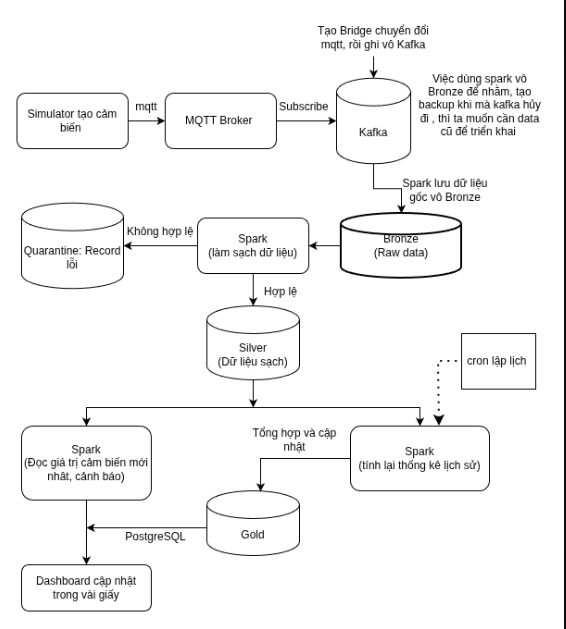
\includegraphics[width=0.72\linewidth,trim=16 0 2 0,clip]{figures/ch3-overview-author.png}
\caption[Sơ đồ luồng dữ liệu tổng quát của pipeline.]{Sơ đồ luồng dữ liệu tổng
quát của nhóm: Simulator $\rightarrow$ MQTT $\rightarrow$ Kafka $\rightarrow$
Spark $\rightarrow$ Bronze/Silver/Quarantine, nhánh batch tổng hợp Gold và
dashboard. Hình~\ref{fig:architecture} trình bày dạng triển khai cụ thể bằng
Docker Compose; hộp cron là lịch chạy batch Gold trên host.}
\label{fig:dataflow-overview}
\end{figure}

\begin{figure}[t]
\centering
{\setstretch{1}
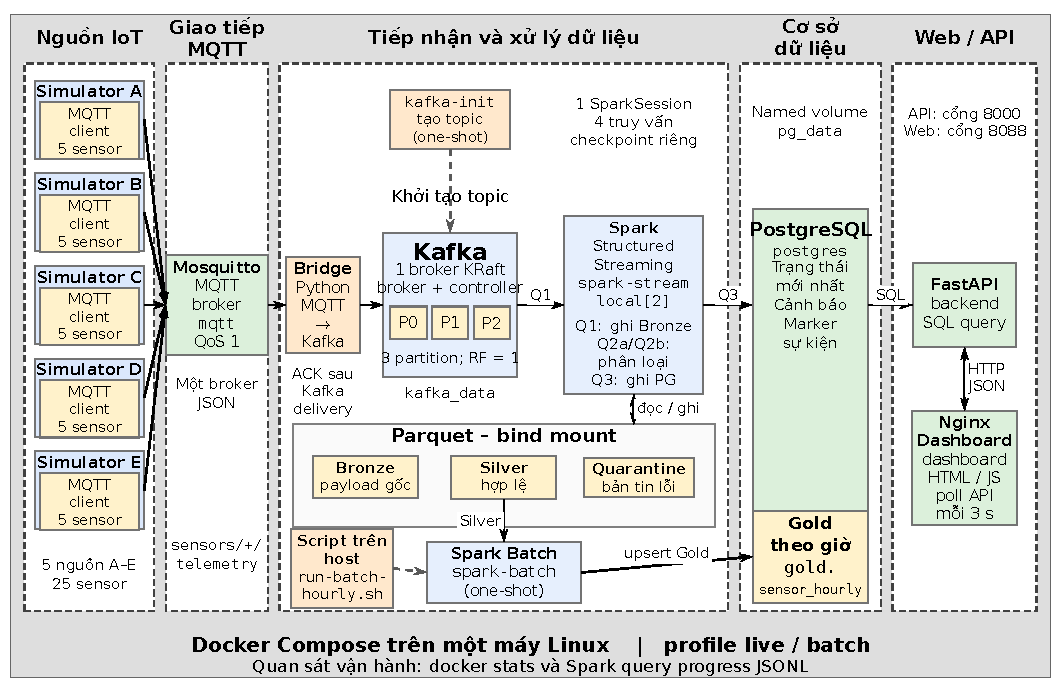
\includegraphics[width=\linewidth]{figures/ch3-deployment-l1.pdf}
}

\caption[Kiến trúc hệ thống năm tầng trên một máy Linux.]{Kiến trúc năm tầng của
pipeline một máy. Simulator phát tập con chỉ số theo loại trạm; Bridge chỉ ACK
MQTT sau Kafka delivery. Một SparkSession chạy Q1/Q2a/Q2b/Q3 với checkpoint riêng.
Bronze/Silver/Quarantine nằm trên Parquet cục bộ; PostgreSQL giữ trạng thái phục
vụ và Gold. Nét đứt là điều phối bằng script. Cron trên host gọi script batch
Gold mỗi giờ; script giữ file lock và chạy được song song với streaming.}
\label{fig:architecture}
\end{figure}

\textbf{Tầng 1 --- Ingestion.} Nhiều container Simulator (mặc định 5, khởi động
qua \texttt{docker compose run} ad-hoc) sinh dữ liệu cảm biến giả lập gồm tập con
của 6 chỉ số môi trường, publish qua MQTT QoS1 tới broker Mosquitto. Mỗi container
dùng tham số \texttt{-{}-prefix} riêng (\texttt{zoneA}\ldots\texttt{zoneE}) để
đảm bảo \texttt{event\_id} không trùng chéo giữa các nguồn. Một Bridge Python
subscribe MQTT, produce vào Kafka topic \texttt{sensor\_raw} (mặc định; phiên tải dài dùng topic riêng \texttt{sensor\_raw\_load15\_20261002}) với cơ chế
\emph{manual ACK}: chỉ gửi PUBACK cho MQTT broker sau khi Kafka báo delivery
thành công (\texttt{acks=all}). Kafka chạy 1 broker KRaft, 3 partition,
replication factor = 1, key phân vùng là \texttt{sensor\_id}, retention tường
minh 1 giờ. Lớp Bridge tách giao thức thiết bị (MQTT) khỏi giao thức xử lý
(Kafka) --- Spark không bao giờ biết MQTT tồn tại.

\textbf{Tầng 2 --- Stream processing.} Một Spark Structured Streaming application
duy nhất chạy ở chế độ \texttt{local[2]} (2 thread) trong container
\texttt{spark-stream}, thực thi đồng thời 4 query chia sẻ chung SparkSession:
Q1 đọc từ Kafka ghi raw payload lossless xuống Bronze Parquet; Q2a đọc Bronze
file stream, validate per-metric, ghi row hợp lệ xuống Silver Parquet; Q2b ghi
row lỗi định danh/thời gian xuống Quarantine Parquet kèm lý do; Q3 đọc Silver file
stream, upsert bảng \texttt{sensor\_latest} và đánh dấu \texttt{processed\_events}
trong PostgreSQL. Mỗi query có checkpoint directory riêng trên bind mount.

\textbf{Tầng 3 --- Storage.} Ba lớp Bronze/Silver/Quarantine lưu dưới dạng
Parquet trên thư mục bind mount cục bộ (\texttt{\$\{DATA\_ROOT\}/bronze},
\texttt{silver}, \texttt{quarantine}), không dùng HDFS hay Delta Lake. PostgreSQL
lưu ba bảng phục vụ: \texttt{sensor\_latest} (giá trị mới nhất per sensor,
upsert idempotent), \texttt{alerts} (cảnh báo do Q3 ghi vào khi phát hiện
vượt ngưỡng), \texttt{processed\_events} (replay marker cho dedup), và
schema \texttt{gold.sensor\_hourly} (aggregate theo giờ từ batch).

\textbf{Tầng 4 --- Batch (kích hoạt bằng script/cron).} Spark batch là container
one-shot (\texttt{spark-batch}, restart policy \texttt{no}) chạy script
\texttt{run-batch.sh -{}-start <UTC> -{}-end <UTC>}, đọc trực tiếp Silver Parquet
và ghi aggregate vào \texttt{gold.sensor\_hourly} bằng
\texttt{ON CONFLICT DO UPDATE} theo khóa sensor--giờ--chỉ số. Chạy lại trên
cùng đầu vào thay thế count/avg/min/max của khóa đó, không cộng dồn. Việc lên lịch hàng giờ không dùng một nền tảng
điều phối riêng: script \texttt{run-batch-hourly} tính cửa sổ giờ UTC vừa kết
thúc và gọi đúng chương trình batch đó; trên máy demo, host chạy nó bằng một
mục cron \texttt{0 * * * *} (Phụ lục~\ref{app:deployment}). Fixture đã
kiểm tra lời gọi thủ công; lịch cron đã được cài và chạy thật một lần trên máy
demo (Mục~\ref{subsec:d5-detail}).
Có hai đường vận hành khác nhau: chuyển mode thủ công bằng
\texttt{run-mode.sh} drain rồi dừng streaming trước khi chạy batch; script
hourly chờ một khoảng grace và dùng file lock, có thể chạy batch đồng thời
với streaming. Vì vậy ngân sách live/batch tách riêng không đại diện cho
tổng giới hạn RAM khi hai container Spark cùng hoạt động.

\textbf{Tầng 5 --- Serving \& Dashboard.} FastAPI backend đọc từ PostgreSQL
và cung cấp bốn nhóm endpoint: \texttt{/api/sensors/latest},
\texttt{/api/alerts}, \texttt{/api/stats} và \texttt{/api/progress}.
Dashboard tĩnh (HTML/JS) qua Nginx
fetch API mỗi 3 giây để hiển thị real-time.

\textbf{Quan sát vận hành.} Thay vì cụm Prometheus/Grafana/JMX Exporter, hệ
thống dùng tiến độ truy vấn Spark (query progress JSONL), thống kê container
qua \texttt{docker stats}, và script \texttt{resource-report.sh} ghi nhận các
chỉ số theo chu kỳ. Chi tiết ở Mục~\ref{subsec:observability-script}.

Lưu ý rằng dữ liệu giữa các tầng không ``tự chảy'': mỗi mũi tên trên
Hình~\ref{fig:architecture} tương ứng một query/job cụ thể.
Hình~\ref{fig:event-flow} làm rõ quyết định phân loại sự kiện tại Q2 và
vị trí xử lý bản trùng trong hai đường Q3 và Gold.

\begin{figure}[H]
\centering
{\setstretch{1}
\begin{tikzpicture}[
  box/.style={draw, rounded corners=2pt, align=center, text width=4.4cm,
    minimum height=1.1cm, fill=blue!6, font=\footnotesize},
  arrow/.style={-{Stealth[length=2.2mm]}, thick},
  lbl/.style={font=\footnotesize, align=center, text width=2.6cm}
]
% Vị trí tương đối: mũi tên luôn bám cạnh hộp dù hộp cao thấp khác nhau.
\node[box, fill=orange!12] (bronze) at (0,0)
  {Bronze: payload nguyên bản\\kèm provenance Kafka/MQTT};
\node[box, below=1.3cm of bronze] (validate)
  {Q2: kiểm tra 4 trường bắt buộc\\định danh và thời gian};
\node[box, fill=red!8, minimum height=1.4cm, below=2.2cm of validate, xshift=-3.0cm] (quar)
  {Quarantine: loại cả bản tin\\lỗi định danh hoặc thời gian};
\node[box, minimum height=1.4cm, below=2.2cm of validate, xshift=3.0cm] (metric)
  {Q2a: kiểm tra từng chỉ số\\chỉ số lỗi $\rightarrow$ NULL\\\texttt{metric\_issues} giữ lý do};
\node[box, fill=orange!12, minimum height=1.4cm, below=1.2cm of metric] (silver)
  {Silver: giữ bản trùng và muộn\\chỉ số vắng theo loại trạm không phải lỗi};
\node[box, fill=green!9, minimum height=1.3cm, below=2.0cm of silver, xshift=-3.0cm] (q3)
  {Q3 $\rightarrow$ PostgreSQL\\khóa duy nhất, latest và cảnh báo};
\node[box, fill=green!9, minimum height=1.3cm, below=2.0cm of silver, xshift=3.0cm] (gold)
  {Batch $\rightarrow$ Gold\\dedup trước khi tổng hợp theo giờ};
\coordinate (split) at ([yshift=-1.15cm]validate.south);
\draw[arrow] (bronze) -- (validate);
\draw[arrow] (validate.south) -- (split) -| (quar.north);
\draw[arrow] (validate.south) -- (split) -| (metric.north);
\node[lbl, anchor=south] at ([xshift=-1.5cm, yshift=1pt]split) {lỗi định danh/\\thời gian};
\node[lbl, anchor=south] at ([xshift=1.5cm, yshift=1pt]split) {4 trường\\hợp lệ};
\draw[arrow] (metric) -- (silver);
\draw[arrow] (silver.south) -- ++(0,-0.8) -| (q3.north);
\draw[arrow] (silver.south) -- ++(0,-0.8) -| (gold.north);
\end{tikzpicture}
}

\caption[Rẽ nhánh sự kiện tại Q2 và phạm vi xử lý bản trùng.]{Rẽ nhánh sự kiện
sau Bronze. Q2b cách ly cả bản tin khi định danh hoặc thời gian không hợp lệ.
Lỗi từng chỉ số được ghi vào \texttt{Silver.metric\_issues}, chỉ số lỗi bị
mask NULL. Silver vẫn giữ bản trùng; Q3 bảo vệ khóa phục vụ khi replay và batch
loại trùng trước khi tính Gold. Chỉ số vắng theo loại trạm không phải lỗi.}
\label{fig:event-flow}
\end{figure}

\subsection{Các thành phần chính và vai trò}

\begin{table}[H]
\centering
\caption{Vai trò và lý do lựa chọn của từng thành phần trong pipeline.}
\label{tab:components}
\begin{tabularx}{\textwidth}{l l X}
\toprule
\textbf{Thành phần} & \textbf{Vai trò} & \textbf{Lý do lựa chọn} \\
\midrule
Simulator (Python) & Sinh tải đa nguồn có kiểm soát & 5 container ad-hoc, fault injection seeded, manifest JSONL \\
Mosquitto & MQTT Broker QoS1 & Giao thức IoT nhẹ, persistent session, phù hợp thiết bị yếu \\
Bridge (Python) & Chuyển MQTT $\rightarrow$ Kafka & Tách giao thức thiết bị khỏi giao thức xử lý, manual ACK after delivery \\
Kafka (KRaft) & Bộ đệm phân tán có thứ tự & Decouple ingestion/xử lý, partition theo key, retention 1h, replay được \\
Spark SS (local{[}2{]}) & Stream processor 4 query & Bronze lossless, validate per-metric, upsert PG, checkpoint riêng \\
Parquet (bind mount) & Lưu trữ Bronze/Silver/Quarantine & Định dạng cột nén, Spark native, không cần HDFS/Delta cho demo 1 máy \\
PostgreSQL & Serving layer + Gold & Upsert idempotent, ACID, FastAPI đọc trực tiếp \\
FastAPI & API backend & Lightweight, async, đọc PG phục vụ dashboard \\
Dashboard (Nginx) & Hiển thị real-time & Static HTML/JS, fetch 3s, không cần framework nặng \\
run-batch-hourly.sh & Kích hoạt batch theo giờ & Script wrapper gọi run-batch.sh với cửa sổ giờ UTC; host chạy bằng cron \\
resource-report.sh & Quan sát vận hành & Đọc docker stats + query progress JSONL, nhẹ hơn Prometheus stack \\
\bottomrule
\end{tabularx}
\end{table}

\section{Data contract và mô hình Bronze--Silver--Gold}
\label{subsec:data-contract}

\subsection{Sensor event schema đa chỉ số}

Mỗi bản tin MQTT là một JSON object mang \emph{vector data-fusion} gồm nhiều
chỉ số môi trường của cùng một cảm biến tại cùng một thời điểm. Contract gồm
4 trường bắt buộc và 6 trường chỉ số tùy chọn (tùy loại cảm biến):

\begin{lstlisting}[language=yaml,basicstyle=\ttfamily\footnotesize,frame=single,
  caption={Sensor event schema (JSON) voi vector da chi so.},label={lst:schema}]
{
  "event_id":       "zoneA-000001",
  "sensor_id":      "zoneA_WEATHER_01",
  "event_time":     "2026-09-18T10:15:32+07:00",
  "ingest_time":    "2026-09-18T03:15:32.120Z",
  "temperature_c":  36.2,
  "humidity_pct":   65.0,
  "co2_ppm":        420.0,
  "pressure_hpa":   1013.25,
  "pm25_ugm3":      12.5,
  "light_lux":      15000.0
}
\end{lstlisting}

Trong đó: \texttt{event\_id} phục vụ deduplication, format
\texttt{\{prefix\}-\{seq:06d\}} tránh trùng giữa các container trong cùng
lần chạy khi prefix khác nhau. Khi chạy lại với seq reset, cần prefix/run ID
mới để không tái dùng định danh của dữ liệu cũ; \texttt{sensor\_id} format
\texttt{\{prefix\}\_\{TYPE\}\_\{NN\}} (TYPE là WEATHER, AIR hoặc MULTI); \texttt{event\_time} là mốc thời gian
thực tế tại cảm biến (dùng cho event-time window); \texttt{ingest\_time} là mốc
producer gắn trước khi gửi. Không mọi bản tin đều có đủ 6 chỉ số --- một trạm
thời tiết có thể chỉ phát nhiệt/ẩm/áp suất/ánh sáng, trong khi trạm chất lượng
không khí phát CO$_2$/PM2.5.

Bảng~\ref{tab:metrics} định nghĩa 6 chỉ số môi trường cùng miền giá trị vật lý
(dùng cho validation/quarantine) và ngưỡng cảnh báo (dùng cho phát hiện alert
ngay trong Q3).

\begin{table}[H]
\centering
\caption{Sáu chỉ số môi trường: ký hiệu, đơn vị, miền vật lý và ngưỡng cảnh báo.}
\label{tab:metrics}
\begin{tabularx}{\textwidth}{l l l l l X}
\toprule
\textbf{Chỉ số} & \textbf{Trường} & \textbf{Đơn vị} & \textbf{Miền vật lý} & \textbf{Ngưỡng alert} & \textbf{Hướng} \\
\midrule
Nhiệt độ & \texttt{temperature\_c} & °C & $[-50, 200]$ & 35 & cao \\
Độ ẩm & \texttt{humidity\_pct} & \%RH & $[0, 100]$ & 80 & cao \\
CO$_2$ & \texttt{co2\_ppm} & ppm & $[0, 5000]$ & 1000 & cao \\
Áp suất & \texttt{pressure\_hpa} & hPa & $[300, 1100]$ & 950 & thấp \\
Bụi mịn & \texttt{pm25\_ugm3} & µg/m³ & $[0, 1000]$ & 35 & cao \\
Ánh sáng & \texttt{light\_lux} & lux & $[0, 200000]$ & --- & không alert \\
\bottomrule
\end{tabularx}
\end{table}

Ma trận 6 chỉ số này được thiết kế để ép thuật toán validation phải tổng quát:
có metric ngưỡng cao (nhiệt, ẩm, CO$_2$, PM2.5), có metric ngưỡng thấp (áp suất),
có metric không có ngưỡng cảnh báo (ánh sáng), miền hẹp/rộng khác nhau, đơn vị
khác nhau. Việc thêm chỉ số dùng chung logic validation/alert, nhưng vẫn cần đồng
bộ registry, schema Spark/PostgreSQL và kiểm thử tương thích.

\subsection{Bronze--Silver--Gold: Parquet và PostgreSQL}

Dữ liệu được tổ chức thành ba lớp Parquet trên bind mount cục bộ
(\texttt{\$\{DATA\_ROOT\}}), cộng một lớp Gold trong PostgreSQL:

\begin{table}[H]
\centering
\caption{Đặc tả ba lớp dữ liệu Bronze/Silver/Gold và Quarantine.}
\label{tab:medallion}
\begin{tabularx}{\textwidth}{l l X}
\toprule
\textbf{Lớp} & \textbf{Định dạng} & \textbf{Nội dung \& quy tắc} \\
\midrule
Bronze & Parquet &
  Raw payload bytes + provenance Kafka/MQTT (topic, partition, offset,
  received\_at\_utc). Lossless: không parse, không dedup, không loại bỏ.
  JSON hỏng được giữ nguyên. Bản lưu thô cục bộ phục vụ đối soát và tái
  xử lý sau khi Kafka hết retention, nếu tệp vẫn còn nguyên vẹn. \\
Silver & Parquet &
  Tập con chỉ số đã parse + chuẩn hóa UTC + flag \texttt{is\_late}.
  Row hợp lệ về bốn trường định danh/thời gian. Chỉ số hỏng = NULL kèm
  \texttt{metric\_issues}; row vẫn được giữ, kể cả row trùng. Chỉ số vắng
  theo loại trạm = NULL nhưng không ghi lỗi. \\
Quarantine & Parquet &
  Row lỗi định danh/thời gian + \texttt{error\_reason}: thiếu
  \texttt{event\_id}/\texttt{sensor\_id} hoặc thiếu/không parse được
  \texttt{event\_time}/\texttt{ingest\_time}. Bổ trợ độc quyền với Silver;
  không chứa lỗi chỉ số của các row đã vào Silver. \\
Gold & PostgreSQL &
  Bảng \texttt{gold.sensor\_hourly}: aggregate avg/min/max/count theo
  \texttt{(sensor\_id, hour\_start, metric)}. \texttt{ON CONFLICT DO UPDATE} theo khóa; rerun trên cùng đầu vào
  không cộng dồn. Khóa vắng trong lần tính lại không tự bị xóa. \\
\bottomrule
\end{tabularx}
\end{table}

\textbf{Quy tắc đặt tên đường dẫn:}
\texttt{\$\{DATA\_ROOT\}/bronze/sensor}, \texttt{silver/sensor},
\texttt{quarantine/sensor}. Checkpoint riêng cho từng query:
\texttt{checkpoints/q1}, \texttt{q2a}, \texttt{q2b}, \texttt{q3}. Toàn bộ nằm
trên bind mount để tồn tại qua restart container.

\section{Môi trường và công cụ}

\subsection{Phiên bản phần mềm}

\begin{table}[H]
\centering
\caption{Phiên bản phần mềm sử dụng trong triển khai.}
\label{tab:versions}
\small
\begin{tabularx}{\textwidth}{l l X X}
\toprule
\textbf{Thành phần} & \textbf{Phiên bản} & \textbf{Image} & \textbf{Ghi chú} \\
\midrule
Apache Kafka & 4.3.1 & official KRaft image & 1 broker, 3 partitions, RF=1~\cite{kafka_docs_4_3} \\
Apache Spark & 4.2.0 & custom image + jar Kafka/JDBC & local{[}2{]}, Structured Streaming~\cite{spark_docs_4_2} \\
PostgreSQL & 17.11 & official image & 1 database (app), schema riêng cho Gold \\
Mosquitto & 2.0.22 & official image & MQTT QoS1, anonymous \\
Python (Bridge/Sim) & 3.12 & custom image & paho-mqtt, confluent-kafka \\
FastAPI & 0.141.1 & custom image & uvicorn, psycopg2 \\
Nginx & 1.27-alpine & custom image & Static dashboard + reverse proxy \\
\bottomrule
\end{tabularx}
\end{table}

\subsection{Cấu hình Docker Compose}

Hệ thống được đóng gói bằng một file \texttt{compose.yaml} với các service
nhóm theo profile:

\begin{lstlisting}[language=yaml,basicstyle=\ttfamily\footnotesize,frame=single,
  caption={Logical services trong compose.yaml.},label={lst:compose}]
# --- Always on (no profile) ---
postgres:                # 1 database: app (serving + gold schemas)
backend:                 # FastAPI serving layer
dashboard:               # Nginx static + reverse proxy

# --- Profile: live ---
mqtt:                    # Mosquitto MQTT broker
simulator:               # Template; spawn via docker compose run
bridge:                  # MQTT -> Kafka pass-through
kafka:                   # KRaft single broker
kafka-init:              # One-shot topic creation
spark-stream:            # 4 queries Q1-Q3 in one SparkSession

# --- Profile: batch ---
spark-batch:             # One-shot hourly Gold aggregation
                         # (started by run-batch-hourly.sh + host cron)
\end{lstlisting}

\textbf{Bind mount và volume:} đường dẫn data plane được bind mount từ
\texttt{\$\{DATA\_ROOT\}} trên host vào \texttt{/data/bigdata} trong mọi
container, gồm sáu thư mục con \texttt{bronze}, \texttt{silver},
\texttt{quarantine}, \texttt{checkpoints}, \texttt{logs} và
\texttt{control}. Kafka và
PostgreSQL data dùng named volumes. Giới hạn bộ nhớ: Spark 2560m, Kafka 1024m,
PostgreSQL 512m, Backend 256m, Bridge 128m, MQTT 64m, Simulator 64m, Dashboard
64m --- tổng live mode khoảng 4,6~GiB.

\textbf{Chuyển đổi mode:} script \texttt{run-mode.sh} chuyển giữa
live/batch mà không xóa volume hay checkpoint. Khi chuyển sang
batch, script drain pipeline live trước (stop simulator + bridge, đợi
Spark tiêu hết backlog Kafka qua progress log, rồi SIGTERM spark-stream).

\subsection{Trạng thái triển khai và phạm vi thực nghiệm}

Mô tả cơ chế không đồng nghĩa mọi tình huống đã được thử ở tải dài.
Bảng~\ref{tab:implementation-evidence} phân biệt hai trạng thái này.

\begin{table}[H]
\centering
\caption{Cơ chế đã có và phạm vi bằng chứng được báo cáo.}
\label{tab:implementation-evidence}
\small
\begin{tabularx}{\textwidth}{>{\raggedright\arraybackslash}p{3.3cm} *{2}{>{\raggedright\arraybackslash}X}}
\toprule
\textbf{Cơ chế} & \textbf{Bằng chứng hiện có} & \textbf{Giới hạn} \\
\midrule
Q1--Q3, lưu trữ và serving & Phiên sạch bốn giờ có dữ liệu và log. & Chưa có rate-sweep hoặc latency tới dashboard. \\
Validation và phục hồi & Fixture D2/D3 và D6 trong test report. & Chưa tương đương lỗi hoặc sự cố dưới tải dài. \\
Gold, rerun và file lock & 450 nhóm Gold được đối soát; D4/D5 kiểm tra rerun và lock ở fixture. & Đối soát 450 nhóm không tự xác nhận rerun workload dài hoặc cron. \\
Watermark mở rộng, policy thích nghi & Thiết kế ở Chương~\ref{chap:background}. & Chưa triển khai và chưa có số đo. \\
\bottomrule
\end{tabularx}
\end{table}

Thời gian thực trong phạm vi này là xử lý liên tục bằng micro-batch gần
thời gian thực, không phải bảo đảm deadline cứng cho từng event.
Checkpoint và khóa duy nhất hỗ trợ resume/idempotency trong phạm vi tương
ứng, không tạo giao dịch nguyên tử xuyên Kafka--Parquet--PostgreSQL.
Với \texttt{failOnDataLoss=false}, việc query tiếp tục chạy không thay
thế đối soát khi offset Kafka đã hết retention.

\section{Cài đặt chi tiết}

\subsection{Simulator đa nguồn}

Simulator (\texttt{simulator/producer.py}) publish canonical payload qua MQTT
QoS1~\cite{mqtt_v311_spec}, topic \texttt{sensors/<sensor\_id>/telemetry}.
Tốc độ \texttt{RATE} là event/s của cả container, luân phiên giữa các sensor;
5 container đặt rate 2 tạo khoảng 10 event/s tổng, không phải 50 event/s. Tham số
\texttt{-{}-fault-inject} với seed xác định tạo tỷ lệ lỗi có kiểm soát:
2\% duplicate, 1\% missing field, 1\% non-numeric, 1\% invalid timestamp,
1\% out-of-bounds, 0,5\% late 30 s, 0,5\% late 5 phút. Mỗi container ghi manifest
JSONL làm source of truth để đối chiếu sent-vs-delivered.

Khi chạy 5 container song song, mỗi container nhận \texttt{-{}-prefix zoneX}
để \texttt{event\_id} = \texttt{zoneX-\{seq:06d\}} không trùng chéo.

\subsection{Bridge MQTT \texorpdfstring{$\rightarrow$}{sang} Kafka}

Bridge (\texttt{bridge/bridge.py}) subscribe MQTT filter
\texttt{sensors/+/telemetry} ở QoS1, persistent session. Luồng: message đến
$\rightarrow$ bounded queue (5000) $\rightarrow$ worker produce vào Kafka với
\texttt{acks=all}, \texttt{enable.idempotence=true}, key = \texttt{sensor\_id}.
\textbf{Chỉ ACK MQTT sau khi Kafka delivery callback báo thành công} --- nếu
bridge crash giữa produce và ACK, broker redeliver, downstream dedup gánh.
Payload được chuyển nguyên bản; Bridge lấy key từ topic hoặc định danh
trong JSON. Không cấu hình \texttt{partitioner} riêng, nên không được giả
định thuật toán Murmur2: client librdkafka mặc định dùng
\texttt{consistent\_random} (CRC32 cho key có giá trị)~\cite{librdkafka_config}.

\subsection{Spark streaming app (4 queries)}
\label{subsec:spark-stream}

Một SparkSession duy nhất (\texttt{spark/jobs/stream\_app.py}) chạy 4 query
với trigger interval mặc định 5 giây:

\textbf{Q1 (Kafka $\rightarrow$ Bronze):} đọc topic \texttt{sensor\_raw}, ghi
\texttt{raw\_payload} lossless + provenance Kafka/MQTT xuống Parquet. Không
parse, không dedup. Bronze là bản lưu thô cục bộ phục vụ đối soát và tái
xử lý, tồn tại qua restart container nhờ bind mount. Do cùng nằm trên một
máy vật lý, Bronze và checkpoint chưa phải backup độc lập bảo vệ trước
hỏng ổ đĩa hoặc mất máy. Khả năng đó cần bản sao ở thiết bị hoặc miền lỗi
khác, kèm kiểm thử khôi phục.

\begin{lstlisting}[language=yaml,basicstyle=\ttfamily\footnotesize,frame=single,
  caption={Pseudo-code Q1: Kafka to Bronze.},label={lst:q1}]
raw = (spark.readStream
         .format("kafka")
         .option("kafka.bootstrap.servers", KAFKA_BOOTSTRAP)
         .option("subscribe", "sensor_raw")
         .option("startingOffsets", "earliest")
         .option("includeHeaders", "true")
         .option("failOnDataLoss", "false")
         .option("maxOffsetsPerTrigger", "20000")
         .load())

# MQTT_TOPIC_EXPR extracts mqtt_topic from Kafka headers.
bronze = raw.select(
    col("value").alias("raw_payload"),
    expr(MQTT_TOPIC_EXPR).alias("mqtt_topic"),
    col("topic").alias("kafka_topic"),
    col("partition").alias("kafka_partition"),
    col("offset").alias("kafka_offset"),
    col("timestamp").alias("kafka_timestamp"),
    current_timestamp().alias("received_at_utc")
)

(bronze.writeStream
   .format("parquet")
   .option("path", BRONZE_PATH)
   .option("checkpointLocation", CP_Q1)
   .trigger(processingTime=TRIGGER_INTERVAL)
   .start())
\end{lstlisting}

\textbf{Q2a/Q2b (Bronze $\rightarrow$ Silver / Quarantine):} đọc Bronze file
stream, áp dụng validation per-metric qua \texttt{build\_validity\_columns()}
(PySpark) đồng bộ với \texttt{classify\_event()} (pure Python reference).
Validation kiểm tra bốn trường bắt buộc: \texttt{event\_id},
\texttt{sensor\_id}, \texttt{event\_time} và \texttt{ingest\_time}. Hai nhánh
Q2a/Q2b bổ trợ độc quyền theo tính hợp lệ của định danh/thời gian. Với mỗi
chỉ số có mặt, lỗi non-numeric hoặc ngoài miền vật lý chỉ mask chỉ số đó
thành NULL và ghi lý do vào \texttt{metric\_issues}; bản tin vẫn vào Silver.
Chỉ số vắng theo loại trạm không sinh lỗi. Silver không loại trùng.

\textbf{Q3 (Silver $\rightarrow$ PostgreSQL):} đọc Silver file stream qua
\texttt{foreachBatch}; mỗi micro-batch gọi hàm
\texttt{pg\_sink.apply\_stream\_batch()} thực hiện staging write rồi
transactional upsert \texttt{sensor\_latest} (tie-break theo
\texttt{event\_time}, \texttt{received\_at}, \texttt{event\_id}), insert
idempotent vào \texttt{processed\_events}, và tính cảnh báo ngay trong cùng
transaction theo mô tả ở Mục~\ref{subsec:alert-q3}.

Hình~\ref{fig:q3-transaction} phân biệt bước ghi staging qua JDBC và giao
dịch cập nhật bảng phục vụ. Khóa duy nhất bảo vệ cardinality khi replay,
nhưng bộ đếm duplicate có thể tăng nếu cùng micro-batch được áp dụng lại.
Không có giao dịch nguyên tử chung giữa Kafka, Parquet và PostgreSQL.

\begin{figure}[H]
\centering
{\setstretch{1}
\begin{tikzpicture}[
  box/.style={draw, rounded corners=2pt, align=center, fill=blue!6,
    text width=5.8cm, minimum height=1.1cm, font=\footnotesize},
  table/.style={box, text width=3.8cm, fill=green!9, minimum height=2.9cm},
  arrow/.style={-{Stealth[length=2.2mm]}, thick},
  lbl/.style={font=\footnotesize, fill=white, inner sep=2pt}
]
% Ba bảng cùng chiều cao, căn giữa theo alerts; mũi tên bám cạnh hộp.
\node[box, fill=orange!12] (silver) at (0,0) {Silver Parquet: micro-batch của Q3};
\node[box, minimum height=1.35cm, below=1.3cm of silver] (staging)
  {\texttt{staging\_stream\_events}\\TRUNCATE đã commit\\JDBC ghi staging};
\node[table, below=2.3cm of staging] (alerts)
  {\texttt{alerts}\\khóa: \texttt{(event\_id,rule\_id)}\\\texttt{DO NOTHING} khi trùng\\mỗi chỉ số vượt ngưỡng một dòng};
\node[table, left=0.45cm of alerts] (latest)
  {\texttt{sensor\_latest}\\khóa: \texttt{sensor\_id}\\một winner/sensor\\event mới hơn ghi đè};
\node[table, right=0.45cm of alerts] (processed)
  {\texttt{processed\_events}\\khóa: \texttt{event\_id}\\một marker/event\\tăng bộ đếm khi replay};
\node[box, fill=green!9, below=1.3cm of alerts] (commit)
  {COMMIT thay đổi trong cả ba bảng\\hoặc ROLLBACK khi có lỗi};
\begin{pgfonlayer}{background}
\node[draw=green!50!black, rounded corners=3pt, inner xsep=8pt, inner ysep=16pt,
  fit=(latest)(alerts)(processed)(commit)] (frame) {};
\end{pgfonlayer}
\draw[arrow] (silver) -- node[right,lbl] {\texttt{foreachBatch}} (staging);
\draw[arrow] (staging.south) -- ++(0,-0.7) -| (latest.north);
\draw[arrow] (staging.south) -- (alerts.north);
\draw[arrow] (staging.south) -- ++(0,-0.7) -| (processed.north);
\draw[arrow] (latest.south) -- ++(0,-0.6) -| (commit.north);
\draw[arrow] (alerts.south) -- (commit.north);
\draw[arrow] (processed.south) -- ++(0,-0.6) -| (commit.north);
% Tiêu đề đặt ở cạnh dưới khung để không bị mũi tên đi vào cắt ngang.
\node[font=\footnotesize\bfseries, fill=white, inner sep=3pt] at (frame.south)
  {Giao dịch PostgreSQL: ba bảng, một commit};
\node[align=center, text width=13.5cm, font=\footnotesize, below=0.8cm of frame]
  {Silver và JDBC staging nằm ngoài giao dịch này. Kafka, Parquet và PostgreSQL\\
   không có một phép commit nguyên tử chung cho toàn pipeline.};
\end{tikzpicture}
}

\caption[Phạm vi giao dịch và khóa duy nhất trong Q3.]{Phạm vi giao dịch của
Q3: sau bước ghi staging, các lệnh cập nhật latest, chèn alert và ghi marker
được commit hoặc rollback trong cùng giao dịch PostgreSQL. Silver vẫn giữ
bản trùng; khóa duy nhất và quy tắc chọn winner bảo vệ trạng thái phục vụ.}
\label{fig:q3-transaction}
\end{figure}

\subsection{Cảnh báo theo ngưỡng trong Q3}
\label{subsec:alert-q3}

Phát hiện cảnh báo nằm ngay trong \texttt{foreachBatch} của Q3, dùng chung
bảng ngưỡng cấu hình với validation: mỗi dòng Silver được đối chiếu với
ngưỡng của từng chỉ số (kèm hướng vượt ngưỡng --- cao hoặc thấp, và chỉ số
không có ngưỡng như ánh sáng thì bỏ qua). Mỗi cặp (event, chỉ số vượt
ngưỡng) sinh một dòng trong bảng \texttt{alerts} với khóa chính
\texttt{(event\_id, rule\_id)} + \texttt{ON CONFLICT DO NOTHING} để đảm bảo
idempotency khi replay. Ngưỡng được khai báo tập trung theo cấu hình (thêm chỉ số cần đồng bộ
registry, schema và test; thuật toán cảnh báo vẫn dùng cùng logic), nhưng không tách thành
bước tiêu thụ riêng: cảnh báo chia sẻ transaction với upsert
\texttt{sensor\_latest}, nên một micro-batch hoặc ghi đủ cả latest lẫn alert,
hoặc không ghi gì --- không có trạng thái nửa vời giữa hai bảng.

\subsection{Spark batch (Silver \texorpdfstring{$\rightarrow$}{sang} Gold)}

Container \texttt{spark-batch} chạy one-shot \texttt{batch.py -{}-start <UTC>
-{}-end <UTC>}, đọc Silver Parquet trong khoảng giờ, loại trùng theo
\texttt{event\_id} bằng tie-break xác định, chuyển sang chiều metric và bỏ
NULL, rồi tính avg/min/max/count nhóm theo
\texttt{(sensor\_id, hour\_start, metric)}. Kết quả được ghi vào \texttt{gold.sensor\_hourly} bằng
\texttt{ON CONFLICT DO UPDATE}. Chạy lại trên cùng đầu vào thay thế giá trị
theo từng khóa, không cộng dồn. Đây không phải phép thay thế toàn cửa sổ:
khóa không xuất hiện trong lần tính lại không tự bị xóa.

\subsection{Điều phối batch bằng script và cron}

Không dùng nền tảng điều phối riêng. Script
\texttt{scripts/run-batch-hourly.sh} tính cửa sổ giờ UTC vừa kết thúc
(\texttt{[hh:00, hh+1:00)}), chờ grace (mặc định 60 giây) sau biên giờ, rồi gọi đúng
chương trình \texttt{run-batch.sh} với cặp tham số \texttt{-{}-start}/\texttt{-{}-end}
đó. Trên host demo, một mục cron (\texttt{0 * * * *}) gọi script mỗi giờ; mục
này đã được cài và chạy thật hai lần liên tiếp (Mục~\ref{subsec:d5-detail}),
không chỉ dừng ở fixture.
Script tự từ chối khi một batch trước đó chưa xong (file lock trong
\texttt{control/}), nên không cần cơ chế \texttt{max\_active\_runs} của một
scheduler bên ngoài. Hourly không drain/dừng streaming như đường chuyển mode thủ công; grace
không đảm bảo mọi late event đã có mặt, nên có thể rerun cửa sổ khi cần.
Cách dùng script giảm số dịch vụ điều phối, phù hợp pipeline một máy.

\subsection{Quan sát vận hành bằng script}
\label{subsec:observability-script}

Script \texttt{resource-report.sh} thu thập \texttt{docker stats} (CPU/RAM per
container), đọc \texttt{stream-progress.jsonl} (Spark query progress gồm
numInputRows, offsets), và ghi kết quả theo chu kỳ. Script
\texttt{stats\_parse.py} hỗ trợ parse output. Không cần Prometheus/Grafana
stack --- phù hợp ngân sách RAM một máy.

\subsection{Cấu hình then chốt}

\begin{table}[H]
\centering
\caption{Các cấu hình then chốt và lý do.}
\label{tab:configs}
\begin{tabularx}{\textwidth}{l l X}
\toprule
\textbf{Mục} & \textbf{Giá trị} & \textbf{Lý do} \\
\midrule
Kafka \texttt{acks} & all & Đảm bảo delivery trước khi Bridge ACK MQTT \\
Kafka \texttt{retention.ms} & 1 giờ & Đủ cho bài demo dừng Spark 60s, tiết kiệm disk \\
Kafka partitions & 3 & Chia tải song song, key = sensor\_id \\
Bridge queue & 5000 & Bounded backpressure, drop-không-ACK khi đầy \\
Spark trigger & 5 giây & Cân bằng latency vs overhead \\
Spark maxOffsetsPerTrigger & 20000 & Tránh micro-batch quá lớn \\
Spark mode & local{[}2{]} & 2 thread; cần rate-sweep để xác định capacity \\
Checkpoint dir & bind mount & Tồn tại qua restart, không cần HDFS \\
PG upsert & ON CONFLICT & Idempotent, replay-safe \\
Gold batch & upsert theo khóa & Rerun trên cùng đầu vào không cộng dồn \\
\bottomrule
\end{tabularx}
\end{table}

Chương tiếp theo trình bày phương pháp benchmark và kết quả đánh giá theo năm RQ.

\chapter{Kết quả và đánh giá}
\label{chap:results}

Chương này trình bày phương pháp đánh giá và kết quả theo năm RQ ở
Chương~\ref{chap:introduction}. Số liệu runtime được đối chiếu từ
\texttt{summary.json}, \texttt{bronze-summary.json}, health check, tiến độ
Spark và resource report của phép chạy dài ngày 02/10/2026. Nội dung báo cáo
được biên tập từ snapshot tài liệu tại commit \texttt{6343a18}; metadata của
runtime ghi commit \texttt{dc1c34d1b365f3dcf22e949c2ab0b166582231ac}, nên hai
provenance được giữ tách biệt. Kết quả fixture được trích từ
\texttt{implementation/docs/TEST\_REPORT.md}, cập nhật ngày 01/10/2026.
Hai nguồn được tách riêng vì workload, thời lượng và mục đích khác nhau.
Các kịch bản chưa chạy được trình bày như kế hoạch kiểm chứng, theo thực
hành benchmark trong~\cite{kafka_patterns_benchmark_2025,shufflebench_2024,
fault_recovery_stream_2024}; không gán số minh họa thành kết quả thực nghiệm.
Các biểu đồ là cách biểu thị lại số liệu đã đối chiếu trong evidence, không
phải phép đo mới.

\section{Phương pháp benchmark}

\subsection{Thiết kế thực nghiệm}

Benchmark gồm bảy kịch bản chạy được trên một máy, mỗi kịch bản nhắm vào
một hoặc nhiều RQ. Các kịch bản được thiết kế theo nguyên tắc: mọi tham
số cấu hình (partition, replication factor, message size, workload shape)
phải được ghi tường minh để đảm bảo tính tái lập, theo khuyến nghị
của~\cite{kafka_patterns_benchmark_2025}:

\begin{table}[H]
\centering
\caption{Mapping giữa kịch bản benchmark và RQ.}
\label{tab:benchmark-rq}
\small
\begin{tabularx}{\textwidth}{l l c X}
\toprule
\textbf{Kịch bản} & \textbf{Biến độc lập} & \textbf{RQ} & \textbf{Mục đích} \\
\midrule
Smoke & 5 sim $\times$ 10 evt/s & --- & Xác nhận pipeline chạy đúng end-to-end \\
Đa nguồn & 5 sim đồng thời, offset/partition & RQ-B & Cân bằng tải 3 partition theo sensor\_id \\
Backlog \& recovery & Dừng Spark 60s, đo backlog & RQ-C & Vai trò lớp đệm Kafka, catch-up time \\
Bão hoà ingestion & Rate thấp, quanh điểm đã đo, rồi cao hơn & RQ-A/B & Điểm bão hoà Bridge queue / Spark local{[}2{]} \\
Partition scaling & 1 vs 3 vs 6 partition & RQ-B & Ảnh hưởng song song hoá Q1 throughput \\
Veracity injection & Fault profile seeded per-metric & RQ-D & Dedup, late, bad record per-metric; kế toán record \\
Batch rerun & Chạy lại cùng cửa sổ giờ & RQ-E & Chạy lại không cộng dồn; độ trễ Gold \\
\bottomrule
\end{tabularx}
\end{table}

Cấu hình mặc định cho mọi kịch bản (reporting checklist theo
~\cite{kafka_patterns_benchmark_2025}): 1 Kafka broker KRaft, 3 partition,
RF=1, retention 1 giờ; 1 Bridge queue 5000; Spark local{[}2{]}, trigger 5s,
maxOffsetsPerTrigger 20000; payload là tập con của 6 chỉ số theo loại trạm;
5 simulator
container prefix zoneA--E.

\subsection{Metric thu thập}

Metric được chia thành mười nhóm, thu thập từ query progress
JSONL~\cite{spark_docs_4_2}, \texttt{docker stats}, và các lệnh Kafka
CLI~\cite{kafka_docs_4_3}:

\begin{table}[H]
\centering
\caption{Bộ metric thu thập theo nhóm.}
\label{tab:metrics-results}
\footnotesize
\begin{tabularx}{\textwidth}{l X l}
\toprule
\textbf{Nhóm} & \textbf{Metric} & \textbf{Nguồn} \\
\midrule
Ingestion &
  produced events/s, bytes/s, failed sends &
  Simulator manifest \\
Kafka &
  end-offset/partition, consumer lag, retention usage &
  Kafka CLI + resource-report \\
Spark &
  numInputRows, processedRowsPerSecond, batchDuration &
  stream-progress.jsonl \\
Bridge &
  queue\_full rate, delivery success/fail, redeliver count &
  bridge-deliveries.jsonl \\
Lateness &
  p50/p95/p99 của $t^{r} - t^{e}$
  (\texttt{received\_at\_utc} $-$ \texttt{event\_time}) &
  Phân tích timestamp Bronze/payload \\
State &
  checkpoint size; watermark/state khi có query dùng chúng &
  Filesystem; Spark progress \\
Quality &
  quarantine ratio theo row; metric-issue, late và duplicate ratio &
  Silver/Quarantine row count \\
Reliability &
  lost events, duplicate events &
  manifest vs processed\_events \\
Recovery &
  thời gian từ restart đến lag = 0 và rate $\geq$ 90\% baseline &
  stream-progress.jsonl \\
Compute &
  CPU\%, RAM per container &
  \texttt{docker stats} \\
\bottomrule
\end{tabularx}
\end{table}

\subsection{Công thức tính}
\label{subsec:formulas}

Báo cáo dùng một taxonomy nhất quán với Mục~\ref{subsec:event-tuple}: ba đại
lượng đo ``độ trễ'' khác nhau, không gộp chung thành một con số.

\textbf{Ingestion lateness} (trễ vào, mức event): theo đúng định nghĩa
Ct.~\ref{eq:observed-lateness},
\begin{equation}
  L_i = \max\bigl(0,\ t^{r}_i - t^{e}_i\bigr),
  \label{eq:ingestion-lateness}
\end{equation}
tính từ \texttt{received\_at\_utc} (thời điểm Spark Q1 nhận từ Kafka) và
\texttt{event\_time} của payload. Đây là đại lượng đo được trực tiếp từ hai
timestamp của từng event; nó \emph{không} đồng nhất với lateness so với
watermark: một event được coi là ``đến sau watermark'' khi tại thời điểm đến,
watermark $W_Q$ của query đã vượt qua event time của nó
(Mục~\ref{subsec:watermark}).

\textbf{Ingestion lag} (trễ vào, mức luồng):
\begin{equation}
  \mathrm{Lag}_{\text{partition}} = \mathrm{LEO} - \mathrm{currentOffset}
  \label{eq:consumer-lag}
\end{equation}
trong đó LEO (Log End Offset) là vị trí cuối cùng của log Kafka partition,
còn \texttt{currentOffset} là vị trí Spark Q1 đang đọc tới. Lag có đơn vị là số bản ghi chưa được Q1 đọc, không phải giây; khi
input rate liên tục vượt processing capacity, lag tăng tuyến tính thay vì tự
tiêu tan~\cite{confluent_optimize_clients}.

\textbf{Publication latency} (trễ ra, mức window): thời điểm một aggregate
xuất hiện ở Gold so với thời điểm cửa sổ đó kết thúc theo event time:
\begin{equation}
  \mathrm{PubLatency}_m = t^{o}_m - \mathrm{end}(W_m),
  \label{eq:publication-latency}
\end{equation}
với $t^{o}_m$ là thời điểm dòng aggregate của $W_m$ được ghi vào
\texttt{gold.sensor\_hourly}. Vì Gold job là batch hourly, publication latency
tồn tại ở mức cửa sổ giờ, không phải mức micro-batch streaming.

Với mỗi phân phối, báo cáo dùng p50, p95 và p99 để đặc trưng
~\cite{iot_stream_latency_2021}.

Throughput tức thời:
\begin{equation}
  \mathrm{Throughput}(t) = \frac{N_{\text{processed}}(t)}{\Delta t}
  \label{eq:throughput}
\end{equation}
trong đó $N_{\text{processed}}(t)$ là số record được job xử lý
trong cửa sổ trượt $\Delta t$ (ví dụ 10 giây).

\subsection{Metric chất lượng (rolling, per-metric)}
\label{subsec:quality-metrics}

Metric chất lượng cần phân biệt cấp bản tin và cấp chỉ số. Trong cùng
cửa sổ đối soát đã drain, gọi $N_B$, $N_S$, $N_Q$ là số occurrence ở Bronze,
Silver và Quarantine. Theo phân loại Q2, kiểm tra $N_B=N_S+N_Q$; bản trùng
không biến mất tại Silver. Các tỷ lệ dự kiến cho quality meta-stream
\cite{stream_daq_2024} được định nghĩa như sau:
\begin{equation}
\begin{aligned}
  \rho_{\mathrm{late}} &= \frac{N_{S,\mathrm{late}}}{N_S}, &
  \rho_{\mathrm{dup}} &= \frac{N_S-N_{S,\mathrm{unique}}}{N_S},\\
  \rho_{\mathrm{inv},m} &= \frac{N_{S,\mathrm{issue},m}}{N_{S,\mathrm{present},m}}, &
  \rho_{\mathrm{quar}} &= \frac{N_Q}{N_B}.
\end{aligned}
\label{eq:quality-ratios}
\end{equation}
$N_{S,\mathrm{late}}$ đếm flag \texttt{is\_late} với ngưỡng $\ell=60$ giây;
$N_{S,\mathrm{unique}}$ đếm \texttt{event\_id} phân biệt trong Silver.
$N_{S,\mathrm{issue},m}$ đếm reason của metric $m$ trong
\texttt{Silver.metric\_issues}; $N_{S,\mathrm{present},m}$ chỉ đếm các row
Silver mà payload gốc có metric đó. Có thể nối provenance Bronze để xác
định chỉ số có mặt trước masking. Chỉ số vắng theo loại trạm không thuộc
mẫu số này và không được xem là lỗi. Nếu mẫu số bằng 0, tỷ lệ để trống.

Quarantine chứa lỗi định danh/thời gian ở cấp cả bản tin; không lấy
out-of-bounds của metric từ Quarantine. Bộ đếm \texttt{duplicate\_count}
trong PostgreSQL bao gồm replay Q3, nên không dùng trực tiếp nó để suy ra
tỷ lệ inject tại nguồn. Các tỷ lệ rolling là thiết kế đánh giá cho policy
đề xuất; fixture hiện có xác nhận một số count, chưa xác nhận policy thích nghi.

\section{Kết quả đo runtime trên máy mục tiêu}
\label{sec:measured-runtime}

Phép chạy dài được dùng để quan sát khối lượng và trạng thái ổn định của
pipeline. Năm simulator A--E phát đồng thời vào MQTT; Bridge chuyển tiếp
sang topic Kafka của phiên chạy; Spark Structured Streaming ghi Bronze,
Silver, Quarantine và PostgreSQL theo các query Q1--Q3. Thời lượng nguồn là
14.400 giây cho mỗi nguồn, tương đương bốn giờ. Fault injection được tắt để
đối soát dữ liệu sạch và quan sát khả năng drain của pipeline.

\begin{table}[H]
\centering
\caption{Tóm tắt khối lượng và trạng thái runtime của phiên chạy dài.}
\label{tab:measured-runtime}
\small
\begin{tabularx}{\textwidth}{l X}
\toprule
\textbf{Đại lượng} & \textbf{Giá trị đo được} \\
\midrule
Thời lượng phát & 14.400 s (4 giờ) \\
Nguồn phát & 5 nguồn, 5 sensor logic mỗi nguồn, tổng 25 sensor \\
Tốc độ sự kiện & 3.523,76 event/s tổng; 705 event/s mỗi nguồn theo cấu hình \\
Sự kiện đã phát & 50.760.004 bản ghi và 50.760.004 \texttt{event\_id} phân biệt \\
Payload & 16.226.141.856 byte tại nguồn, Bridge và Bronze; trung bình 319,66 byte/event \\
Bronze & 50.760.004 dòng, 8.647 file Parquet \\
Silver & 50.760.004 dòng, 5.765 file Parquet \\
Quarantine & 0 dòng; phù hợp với việc tắt fault injection \\
Cấu hình xử lý & Kafka 3 partition, Spark \texttt{local[2]}, trigger 5 s, các cap baseline đã ghi trong metadata \\
\bottomrule
\end{tabularx}
\end{table}

Tổng payload 16.226.141.856 byte tương đương 16,226 GB theo quy ước
\(1\,\mathrm{GB}=10^9\) byte. Đây là khối lượng payload thực tế được ghi
nhận trong phiên quan sát, được dùng để kiểm tra tính nhất quán giữa nguồn,
Bridge và Bronze. Đại lượng này là byte payload, không phải dung lượng
Parquet hoặc dung lượng đĩa.

Hình~\ref{fig:payload-accounting} biểu thị cùng tổng payload ở ba điểm đối
soát. Việc bằng nhau về count/byte là evidence ở cấp tổng; chưa thay thế
đối soát anti-join từng \texttt{event\_id} và provenance.

\begin{figure}[H]
\centering
\begin{tikzpicture}
\begin{axis}[
  width=13.0cm, height=6.0cm,
  ybar, bar width=30pt,
  xmin=0.5,xmax=3.5,xtick={1,2,3},
  xticklabels={Nguồn simulator,Bridge,Bronze},
  ylabel={Payload đối soát (GB thập phân)},
  ymin=0,ymax=19,ytick={0,5,10,15},
  ymajorgrids=true,grid style={gray!25},axis lines*=left,
  tick label style={font=\small},label style={font=\small},
  legend style={at={(0.5,1.12)},anchor=south,legend columns=2,
    draw=none,font=\footnotesize},
  every node near coord/.append style={font=\footnotesize}
]
\addplot[fill=blue!55,draw=blue!70!black,
  nodes near coords={\pgfmathprintnumber[fixed,precision=3,use comma]{\pgfplotspointmeta}}]
  coordinates {(1,16.226141856) (2,16.226141856) (3,16.226141856)};
\addlegendentry{Payload đã ghi nhận}
\addplot[red!70!black,dashed,thick,sharp plot] coordinates {(0.5,15) (3.5,15)};
\addlegendentry{Ngưỡng 15 GB/4 giờ}
\end{axis}
\end{tikzpicture}

\caption[Đối soát khối lượng payload qua pipeline.]{Đối soát khối lượng
payload qua ba ranh giới: nguồn phát, Bridge và Bronze đều ghi nhận
50.760.004 event và 16.226.141.856 byte. Hình biểu diễn byte payload của
JSON, không phải dung lượng Parquet hay dung lượng đĩa.}
\label{fig:payload-accounting}
\end{figure}

\begin{table}[H]
\centering
\caption{Thời gian xử lý micro-batch quan sát trong phép tải dài.}
\label{tab:measured-spark}
\begin{tabular}{lrrr}
\toprule
\textbf{Query} & \textbf{Vai trò} & \textbf{P50 (ms)} & \textbf{P95 (ms)} \\
\midrule
\texttt{q1\_bronze} & Kafka $\rightarrow$ Bronze & 344 & 422 \\
\texttt{q2a\_silver} & Bronze $\rightarrow$ Silver & 1.305 & 1.465 \\
\texttt{q2b\_quarantine} & Bronze $\rightarrow$ Quarantine & 537 & 694 \\
\texttt{q3\_pg} & Silver $\rightarrow$ PostgreSQL & 1.457 & 1.651 \\
\bottomrule
\end{tabular}
\end{table}

\begin{figure}[H]
\centering
\begin{tikzpicture}
\begin{axis}[
  width=13.2cm, height=6.6cm,
  ybar, bar width=13pt,
  symbolic x coords={Q1,Q2a,Q2b,Q3}, xtick=data,
  ylabel={Thời gian xử lý micro-batch (ms)},
  ymin=0, ymax=1900, ytick={0,500,1000,1500},
  enlarge x limits=0.2, ymajorgrids=true, grid style={gray!25},
  axis lines*=left, tick label style={font=\small},
  label style={font=\small},
  legend style={at={(0.5,1.12)}, anchor=south, legend columns=2,
    draw=none, font=\small},
  nodes near coords,
  /pgf/number format/.cd,1000 sep={.},/pgfplots/.cd,
  every node near coord/.append style={font=\footnotesize},
  point meta=y
]
\addplot[fill=blue!55,draw=blue!70!black] coordinates
  {(Q1,344) (Q2a,1305) (Q2b,537) (Q3,1457)};
\addlegendentry{P50}
\addplot[fill=orange!65,draw=orange!80!black] coordinates
  {(Q1,422) (Q2a,1465) (Q2b,694) (Q3,1651)};
\addlegendentry{P95}
\end{axis}
\end{tikzpicture}

\caption[P50 và P95 thời gian xử lý micro-batch theo query.]{P50 và P95 theo
query: trích kết quả phiên chạy dài. Q2a và Q3 có thời
gian cao hơn Q1 trong workload sạch này. Các cột đo thời gian micro-batch,
không đo latency đầu-cuối hoặc cộng thành throughput tổng của pipeline.}
\label{fig:microbatch-percentiles}
\end{figure}

Các query Q1--Q3 đều quan sát 2.882 batch trong cửa sổ run. P95 của Q1 là
422 ms, trong khi Q2a và Q3 cao hơn do phải giải mã, chuẩn hóa, kiểm tra
metric và ghi trạng thái phục vụ. Các giá trị này là thời gian xử lý
micro-batch; chúng không phải latency đầu-cuối từ lúc simulator phát event
đến lúc dashboard hiển thị kết quả. Vì vậy không cộng thời gian của bốn query
để tạo ra một con số throughput tổng hợp.

Sau khi nguồn dừng, Kafka offset và Q1 đã được drain về lag bằng không; query
downstream ổn định sau thời gian settle 30 giây và health check trả về
\texttt{status=ok}. Log riêng của run không ghi nhận ERROR/FATAL, PUBACK timeout,
MQTT drop, Spark falling-behind, suspend hoặc OOM. PostgreSQL ghi nhận
50.760.004 marker \texttt{processed\_events} phân biệt cho prefix của run và
878.187 alert. Các số liệu này chứng minh trạng thái phục vụ của Q3 trong
phép tải. Sau khi ingest kết thúc, Gold batch được chạy trên Silver của chính
snapshot này trong cửa sổ [20:00,01:00) UTC ngày 01--02/10/2026, tạo 450
sensor--hour--metric row từ 182.736.016 readings, bao phủ 25 sensor và sáu
metric trong năm cửa sổ giờ. Chạy lại cùng cửa sổ giữ nguyên hai số đếm này,
qua đó kiểm chứng full-replace upsert trên workload dài.

Resource report ghi nhận mức cao nhất trong các mẫu: Spark khoảng
1,878 GiB trên giới hạn 2,5 GiB (75,1\%), PostgreSQL khoảng 466,3 MiB trên
giới hạn 512 MiB (91,1\%), Kafka khoảng 575,3 MiB trên 1 GiB (56,2\%) và
Bridge khoảng 22,46 MiB trên 128 MiB (17,6\%). Dung lượng đĩa trống thấp
nhất được ghi nhận xấp xỉ 21,4 GB; thư mục log và file Parquet là phần tăng
chính trong thời gian chạy. Kết quả này cho thấy PostgreSQL và chính sách
lưu trữ cần được theo dõi khi khối lượng dữ liệu tăng.

Hình~\ref{fig:memory-last-sample} so sánh hai mức sử dụng RAM cao nhất được
ghi nhận với giới hạn container tương ứng; đây là mẫu cực đại trong resource
report, không phải P95 của toàn bộ chuỗi thời gian.

\begin{figure}[H]
\centering
\begin{tikzpicture}
\begin{axis}[
  width=12.0cm,height=5.3cm,
  xbar,bar width=18pt,
  xmin=0,xmax=110,xtick={0,25,50,75,100},
  ymin=0.4,ymax=2.6,ytick={1,2},
  yticklabels={Spark: 1{,}752/2{,}5 GiB,PostgreSQL: 401{,}5/512 MiB},
  xlabel={RAM ở mẫu cuối / giới hạn container (\%)},
  xmajorgrids=true,grid style={gray!25},axis lines*=left,
  tick label style={font=\small},label style={font=\small},
  every node near coord/.append style={font=\footnotesize,anchor=west},
  point meta=x
]
\addplot[fill=blue!55,draw=blue!70!black,
  nodes near coords={\pgfmathprintnumber[fixed,precision=1,use comma]{\pgfplotspointmeta}\%}]
  coordinates {(70.08,1) (78.41796875,2)};
\addplot[gray!70,dashed,thick,sharp plot] coordinates {(100,0.4) (100,2.6)};
\end{axis}
\end{tikzpicture}

\caption[Mức sử dụng RAM cao nhất ghi nhận.]{Mức sử dụng RAM cao nhất trong
resource report: Spark 1,878/2,5 GiB tương đương 75,1\%; PostgreSQL
466,3/512 MiB tương đương 91,1\%. Đây là mẫu cực đại được ghi nhận, không
phải trung bình của bốn giờ.}
\label{fig:memory-last-sample}
\end{figure}

Các file evidence nằm dưới thư mục log của phiên chạy. Tổng số được ghi trong
\texttt{summary.json} và \texttt{bronze-\allowbreak summary.json}; tiến độ
Spark trong \texttt{stream-\allowbreak progress.jsonl}; tài nguyên trong
\texttt{resource-\allowbreak report.jsonl}; health check trong
\texttt{health-check-\allowbreak 20261002.json}. Metadata của run ghi commit
tham chiếu và các tham số nguồn. Các biểu đồ trên trích số liệu đã đối
chiếu từ evidence; không tạo thêm phép đo.

\section{Đánh giá theo RQ và kế hoạch kiểm chứng tiếp theo}

Phần này nối số đo dài với fixture trước đó và ghi rõ nội dung chưa có
đối chứng. Không chuyển kết quả của benchmark khác thành capacity của
máy hiện tại. Bảng~\ref{tab:rq-status} tổng hợp phạm vi evidence.

\begin{table}[H]
\centering
\caption{Trạng thái evidence theo từng câu hỏi nghiên cứu.}
\label{tab:rq-status}
\small
\begin{tabularx}{\textwidth}{l X X}
\toprule
\textbf{RQ} & \textbf{Evidence đã ghi trong repo} & \textbf{Chưa kết luận} \\
\midrule
RQ-A & Một điểm tải 3.523,76 event/s, 16,226 GB/4 giờ; P50/P95 micro-batch &
Capacity tối đa và latency đầu-cuối theo rate-sweep \\
RQ-B & 5 nguồn/25 sensor với 3 partition, \texttt{local[2]} trong run dài &
Lợi ích nhân quả khi đổi partition, core hoặc Bridge \\
RQ-C & Fixture D6 báo PASS 4/4, checkpoint resume và offsets tiến &
Recovery time P95 và loss theo run/provenance riêng \\
RQ-D & Fixture 200 event seeded: 2 lỗi timestamp ở Quarantine;
3 non-numeric + 2 out-of-bounds ở Silver &
Tỷ lệ rolling dài hạn và policy FAST/CAUTIOUS \\
RQ-E & Gold batch workload dài: 450 row/182.736.016 readings, rerun giữ nguyên &
Chi phí batch khi thay đổi kích thước snapshot Silver \\
\bottomrule
\end{tabularx}
\end{table}

\subsection{RQ-A: Throughput và ingestion lateness theo input rate}

Phép tải dài cung cấp một điểm quan sát ổn định ở 3.523,76 event/s tổng.
P95 thời gian micro-batch Q1 là 422 ms, nhưng không phải P95 ingestion
lateness hoặc latency đầu-cuối. Chưa có rate-sweep, vì vậy chưa xác định
được ngưỡng bão hòa của \texttt{local[2]}.

Phép đối chứng tiếp theo giữ message size, số key, cấu hình và thời lượng
quan sát như nhau rồi tăng tốc độ đặt theo từng mức. Tại mỗi mức, đo tốc
độ phát thực, tốc độ Bronze, lag từng partition, Bridge queue/delivery và
phân phối $L_i$ theo Ct.~\ref{eq:ingestion-lateness}. Chỉ gọi là bão hòa
khi tốc độ đầu ra không theo kịp đầu vào và backlog tăng bền vững sau warm-up.
Cách tìm capacity này phù hợp reporting checklist
\cite{kafka_patterns_benchmark_2025}; không gán một giá trị từ minh họa lý
thuyết cho hệ thống đã triển khai.

\subsection{RQ-B: Ảnh hưởng của partition count và đa nguồn}

Run dài chứng minh cấu hình 3 partition/2 thread xử lý được workload đã
nêu; nó không cô lập tác động của số partition. Đối chứng cần so sánh 1,
3 và 6 partition với cùng tổng tốc độ phát, kích thước message và tập key,
rồi so sánh \texttt{local[2]} với \texttt{local[4]} ở cùng cấu hình Kafka.
Đếm đầu ra tại cùng một ranh giới, không cộng input của bốn query vì một
sự kiện có thể đi qua nhiều query.

Cân bằng partition phụ thuộc phân bố key và lưu lượng từng key, không chỉ
số container. Bridge dùng \texttt{sensor\_id} làm key và không chỉ định
partitioner riêng; librdkafka mặc định dùng \texttt{consistent\_random}
(CRC32 cho key có giá trị)~\cite{librdkafka_config}. Nhiều key không đảm bảo cân bằng nếu có hot key.
Cần ghi count/byte của từng partition trước khi kết luận về độ lệch
\cite{confluent_partition_count}. Nhân bản Bridge còn cần MQTT client ID
riêng và chiến lược subscription để tránh cùng nhận toàn bộ bản tin;
Kafka \texttt{client.id} chủ yếu dùng nhận diện/log, không tạo phân phối
subscription MQTT hay đảm bảo dedup xuyên các producer.

\subsection{RQ-C: Backlog và recovery khi dừng Spark}

\texttt{TEST\_REPORT.md} ghi fixture D6 chạy ngày 30/09--01/10/2026 đạt
PASS 4/4: batch 707 $\rightarrow$ 708 sau restart, Kafka offsets tiến,
Bronze tăng và Bridge restart được. Evidence được liệt kê là
\texttt{logs/test-recovery.log}. Đây là kiểm chứng chức năng resume trong
fixture, không phải recovery time được đo của phiên chạy dài.

Phép đo định lượng kế tiếp gồm bốn giai đoạn: lấy baseline; dừng Spark
trong khi nguồn/Bridge/Kafka tiếp tục; khởi động với checkpoint cũ; theo
dõi tới khi lag bằng 0 và tốc độ xử lý trở lại ít nhất 90\% baseline.
Thời gian recovery được tính từ restart, không tính từ lúc bắt đầu dừng.
Nếu tốc độ xử lý sau restart là $\mu$ và tốc độ vào là $\lambda$, điều kiện
bắt kịp là $\mu>\lambda$. Với backlog ban đầu $B_0$ và giả định hai tốc độ
không đổi, thời gian catch-up lý tưởng là
\begin{equation}
  T_{\mathrm{catch}}=\frac{B_0}{\mu-\lambda}.
\end{equation}
Công thức là mô hình kiểm chứng, không phải số đo fixture. Retention phải
bao phủ thời gian dừng và bắt kịp; checkpoint không khôi phục dữ liệu đã
bị Kafka xóa.

\textbf{Loss và duplicate:} đối soát theo run ID, tập event ID và provenance.
Chênh lệch sent/delivered tích lũy qua nhiều run trong test report không
được dùng làm tỷ lệ mất mát. MQTT QoS1 và manual ACK cho phép redelivery;
Silver giữ bản trùng, Q3 bảo vệ cardinality của marker/alert/latest theo
khóa. Không suy ra exactly-once xuyên pipeline từ producer idempotence
hay một giao dịch PostgreSQL.

\subsection{RQ-D: Data veracity --- dedup, late, bad record per-metric}

Fixture D2/D3 trong \texttt{TEST\_REPORT.md}, cập nhật 01/10/2026, sử dụng
200 event với seed 42. Các count được ghi nhận như
Bảng~\ref{tab:rq-d}; chưa có histogram đầy đủ cho mọi chỉ số ở workload dài.

\begin{table}[H]
\centering
\caption{Count lỗi được ghi trong fixture 200 event, seed 42.}
\label{tab:rq-d}
\begin{tabularx}{\textwidth}{l r X}
\toprule
\textbf{Loại lỗi} & \textbf{Count} & \textbf{Nơi ghi nhận và ngữ nghĩa} \\
\midrule
Bad timestamp & 2 & Quarantine: lỗi thời gian loại cả bản tin \\
Non-numeric & 3 & Silver: chỉ số lỗi = NULL, reason trong \texttt{metric\_issues} \\
Out-of-bounds & 2 & Silver: chỉ số lỗi = NULL, reason trong \texttt{metric\_issues} \\
\midrule
Metric issues & 5 & Tổng row Silver có hai loại issue kể trên trong fixture \\
\bottomrule
\end{tabularx}
\end{table}

Manifest fixture còn ghi duplicate 2/200, missing-field 1/200 và late
2/200. Missing-field của simulator xóa một metric có mặt trong payload;
trong contract station-subset, việc thiếu metric đó tự nó không gây
Quarantine. Nếu muốn đánh giá mất trường bắt buộc, phải có fixture riêng
xóa \texttt{event\_id}/\texttt{sensor\_id} hoặc làm hỏng thời gian.
Late 30 giây chưa nhất thiết bật \texttt{is\_late} khi ngưỡng là 60 giây;
không đồng nhất nhãn inject late với count flag late.

Các tỷ lệ chất lượng phải tính theo đúng nơi dữ liệu được lưu: lỗi chỉ
số từ Silver, lỗi định danh/thời gian từ Quarantine, bản trùng từ số
occurrence và số event ID phân biệt. Fixture xác nhận một số count theo
manifest và ngữ nghĩa masking; nó chưa chứng minh lỗi được phân bố đều
trên cả sáu chỉ số hoặc lợi ích của policy thích nghi.

\subsection{RQ-E: Storage và batch rerun determinism}

\textbf{File-stream:} run dài ghi 8.647 file Bronze và 5.765 file Silver.
Để đo tác động của \texttt{maxFilesPerTrigger}, cần giữ cùng snapshot đầu
vào rồi thay riêng cap Q2/Q3, đo thời gian micro-batch, số file xử lý và
backlog. Chưa có đối chứng cap nên không gán P95 hoặc mức tối ưu từ số
minh họa. Byte payload ở Hình~\ref{fig:payload-accounting} không phải byte
Parquet nén và không dùng làm compression ratio.

\textbf{Gold của workload dài:} batch đọc Silver của run
\texttt{load15-clean-20261002} trong cửa sổ [20:00,01:00) UTC ngày
01--02/10/2026 và ghi 450 sensor--hour--metric row từ 182.736.016 readings.
Lần rerun cùng cửa sổ tiếp tục trả về 450 row và 182.736.016 readings, không
cộng dồn. Đây là evidence trực tiếp trên snapshot Silver của phép tải dài;
fixture D4 vẫn được giữ như đối chứng nhỏ với hai file byte-identical
\texttt{gold-run1.csv}/\texttt{gold-run2.csv} (SHA-256 prefix
\texttt{a6e0b181}).

Batch dedup theo event ID trước tổng hợp và dùng
\texttt{ON CONFLICT DO UPDATE} theo khóa sensor--giờ--chỉ số. Rerun trên
cùng đầu vào không cộng dồn count; \texttt{computed\_at} được cập nhật,
không thuộc invariant của giá trị aggregate. Khóa không có trong lần tính
lại không tự bị xóa, nên đây không phải DELETE+INSERT thay toàn cửa sổ.
Fixture D5 xác nhận cửa sổ UTC, grace 60 giây, lock từ chối batch đồng
thời và được nhả sau chạy; cron thật chưa cài.

\section{Phân tích và thảo luận}

\subsection{Mapping giả thuyết với kịch bản đo}
\label{subsec:hypothesis-mapping}

Bốn giả thuyết ở Mục~\ref{subsec:hypotheses} được gắn với kịch bản thực
nghiệm cụ thể:

\begin{table}[H]
\centering
\caption{Mapping giữa giả thuyết và kịch bản/metric cần đo.}
\label{tab:hypothesis-mapping}
\begin{tabularx}{\textwidth}{l l X}
\toprule
\textbf{Giả thuyết} & \textbf{Kịch bản} & \textbf{Metric quyết định} \\
\midrule
H1 (allowed lateness) & Bão hoà ingestion + late injection &
  retention của late event, state rows, publication delay \\
H2 (kế toán chất lượng) & Veracity injection per-metric &
  $\rho_{\mathrm{inv},m}, \rho_{\mathrm{dup}}, \rho_{\mathrm{late}}$ so với tỷ lệ
  inject, kèm sai số lấy mẫu \\
H3 (reconciliation) & Batch rerun determinism &
  sai lệch aggregate trước/sau rerun (kỳ vọng = 0) \\
H4 (adaptive policy) & Bão hoà ingestion kéo dài &
  ablation fixed vs adaptive, adaptive có/không hysteresis \\
\bottomrule
\end{tabularx}
\end{table}

H1 và H4 cần phép đo riêng cho phần mở rộng event-time/adaptive chưa triển
khai. Fixture count và Gold rerun chỉ kiểm chứng một phần H2/H3; không xem
bốn giả thuyết là đã xác nhận đầy đủ.

\subsection{Trade-off chính}

Hệ thống triển khai thể hiện ba trade-off điển hình:

\begin{enumerate}
  \item \textbf{Throughput vs ingestion lateness:} trigger interval nhỏ (1--2s)
        giảm ingestion lateness nhưng tăng overhead micro-batch; trigger lớn
        (30--60s) ngược lại. Cấu hình hiện tại dùng 5s; cần đối chứng nhiều trigger ở cùng workload
        để chọn cấu hình theo mục tiêu latency/throughput;
  \item \textbf{Partition count vs thread count:} partition nhiều tăng song
        song hoá Q1 nhưng bị giới hạn bởi \texttt{local[2]}. Run dài dùng 3 partition/2 thread nhưng chưa chứng minh đây là cấu
        hình tối ưu~\cite{confluent_partition_count};
  \item \textbf{Queue size vs backpressure:} Bridge queue 5000 được dùng trong cấu hình đã đo; queue lớn hơn giảm redeliver nhưng tốn RAM hơn và che giấu
        bottleneck lâu hơn. Khi queue đầy, không ACK giúp giữ khả năng redelivery sau reconnect
        của persistent session; kết quả còn phụ thuộc giới hạn queue và
        persistence của broker, không phải bảo đảm mất mát bằng 0.
\end{enumerate}

\subsection{Giới hạn}

Số liệu trong chương này có ba giới hạn cần ghi nhận:

\begin{itemize}
  \item \textbf{Phạm vi đo runtime còn hẹp}: phép chạy dài đã ghi nhận một
        phiên nhiều nguồn cùng thời gian xử lý micro-batch Q1--Q3, nhưng chưa
        tạo đường cong saturation theo nhiều input rate, chưa full anti-join
        event/provenance, và chưa có rate-sweep để đo chi phí Gold khi kích thước
        snapshot Silver tăng;
  \item \textbf{Một máy, RF=1}: cấu hình 1 Kafka broker KRaft, RF=1 không
        chịu được mất broker. Đây là trade-off chấp nhận cho demo một máy;
  \item \textbf{local{[}2{]}:} Spark chạy 2 thread trong cùng process, không
        đại diện cho cụm phân tán nhiều worker. Khi đo được điểm bão hòa, nó sẽ là giới hạn của cấu hình single-node
        đang thử, không phải giới hạn của Spark nói chung.
\end{itemize}

\subsection{Khuyến nghị cho triển khai thực tế}

\begin{itemize}
  \item Chạy benchmark baseline trước khi thay đổi bất kỳ cấu hình nào,
        lưu kết quả để so sánh;
  \item Ghi tường minh mọi tham số (partition, RF, message size, trigger,
        queue size) trong mỗi bảng số liệu theo reporting
        checklist~\cite{kafka_patterns_benchmark_2025};
  \item Ưu tiên tối ưu Bridge producer (batching, linger.ms) trước khi tăng
        số core Spark~\cite{confluent_optimize_clients};
  \item Theo dõi file-stream backlog Q2/Q3 khi tải tăng --- đây là bottleneck
        đặc trưng của kiến trúc file-stream nối tiếp thay vì đọc thẳng Kafka.
\end{itemize}

Kết luận định lượng về khối lượng payload và trạng thái pipeline ở
Mục~\ref{sec:measured-runtime} được rút ra từ log và summary của phiên chạy
cụ thể. Fixture recovery, fault injection và batch rerun có evidence riêng
ở test report; đường cong saturation và đối chứng scalability vẫn chưa được
đo; H1--H4 chưa được xem là xác nhận đầy đủ chỉ từ phép chạy sạch này.
Chương tiếp theo tổng kết báo cáo và đề xuất hướng phát triển.

\chapter{Kết luận}
\label{chap:conclusion}

\section{Kết quả xây dựng và đánh giá}

Đề tài đã tích hợp nền tảng xử lý IoT trên một máy Linux bằng Docker
Compose: MQTT/Mosquitto tiếp nhận, Bridge chuyển sang Kafka, Spark ghi các
lớp Parquet và trạng thái PostgreSQL, batch tổng hợp Gold theo giờ, còn
FastAPI/dashboard cung cấp đường khai thác. Đóng góp xây dựng nằm ở sự
thống nhất của data contract, định danh, reason lỗi và khóa cập nhật qua
các thành phần. Hệ thống hỗ trợ sáu chỉ số với tập con theo loại trạm.

Phiên có năm nguồn, 25 cảm biến, thời lượng cấu hình bốn giờ, ghi nhận
50.760.004 event và 16.226.141.856 byte payload tại Bronze. Silver có cùng
số dòng; tổng reading là 182.736.016 và tổng lượt cảnh báo là 878.187.
Đây là dữ liệu thực nghiệm sinh bằng simulator, không phải phép đo môi
trường thực. Bộ bằng chứng của phiên tải và các fixture được sử dụng
với phạm vi khác nhau ở Chương~\ref{chap:results}.

\begin{itemize}
 \item \textbf{RQ-A:} throughput nguồn trung bình 3.523,76 event/s và P95
 micro-batch Q1/Q3 là 422/1.650,95 ms mô tả cấu hình đã quan sát. P95
 Kafka--Q1 là 4,761 s; chưa có latency đầu cuối hoặc đường cong tăng tải.
 \item \textbf{RQ-B:} ba partition có tỷ trọng 36/32/32\%; log tài nguyên
 mô tả mức sử dụng tại \texttt{local[2]}. Chưa có đối chứng cô lập ảnh
 hưởng partition/core hoặc xác định điểm bão hòa.
 \item \textbf{RQ-C:} fixture D6 ghi nhận resume từ checkpoint, offset
 tiến và Bridge restart. Chưa đủ bằng chứng recovery time theo phân vị
 hoặc bảo toàn mọi occurrence dưới sự cố trong phiên tải dài.
 \item \textbf{RQ-D:} NULL ở phiên sạch phù hợp loại trạm; D2/D3 kiểm tra
 riêng lỗi định danh/thời gian và lỗi từng chỉ số. Quarantine rỗng không
 chứng minh mọi nhánh lỗi đã được thử ở tải cao.
 \item \textbf{RQ-E:} 450 nhóm Gold khớp phép tổng hợp độc lập từ Silver:
 count/min/max không lệch, sai khác mean lớn nhất khoảng
 $8,26\times10^{-10}$, dưới dung sai $10^{-6}$. Rerun byte-identical được
 ghi ở fixture D4 với 108 dòng/132.844 readings; ở workload dài, tài liệu
 archive chỉ ghi số đếm không đổi sau rerun cùng cửa sổ, chưa có so từng
 khóa, và chưa có kết luận về hiệu năng dashboard.
\end{itemize}

\section{Giới hạn của kết luận}

Kết quả gắn với một máy và một mức tải. Tổng giới hạn bộ nhớ khoảng
4,6 GiB của dịch vụ live là ngân sách cấu hình, không phải tổng RAM đồng
thời đã đo. Đỉnh PostgreSQL 91,07\% giới hạn container là giá trị trong
các mẫu, chưa xác định nút thắt hoặc bảo đảm không có đỉnh ngắn giữa hai
mẫu. Throughput, thời gian batch và khoảng timestamp không đồng nhất.

Bronze và checkpoint nằm trên cùng máy, hỗ trợ tái xử lý và restart
container nhưng chưa bảo vệ trước mất máy/hỏng ổ đĩa. Khóa duy nhất và
transaction bảo vệ phạm vi PostgreSQL, không tạo exactly-once xuyên
pipeline. Gold upsert thay giá trị theo khóa đã tính; khóa vắng trong
lần tính lại không tự bị xóa, nên không phải thay thế toàn cửa sổ.
Cron, full reconciliation của archive và policy thích nghi cần bằng
chứng riêng.

\section{Hướng phát triển}

Ưu tiên tiếp theo là cải thiện phép đo trên kiến trúc một máy đang có.
Bảng~\ref{tab:single-node-roadmap} nêu công việc và đầu ra kiểm chứng; mọi
mục trong bảng là kế hoạch, chưa phải kết quả mới.

\begin{table}[H]
\centering
\caption{Hướng phát triển có thể đo lường trên một máy.}
\label{tab:single-node-roadmap}
\small
\begin{tabularx}{\textwidth}{>{\raggedright\arraybackslash}p{3.1cm} *{2}{>{\raggedright\arraybackslash}X}}
\toprule
\textbf{Công việc} & \textbf{Điều kiện đối chứng} & \textbf{Đầu ra cần lưu} \\
\midrule
Tải và partition/core & Giữ generator/payload; thay một biến; tách warmup, phát và drain. & Throughput, lag, Q1--Q3 duration; lặp cùng điều kiện. \\
CPU/RAM theo thời gian & Ghép timestamp resource log và query progress, giữ khoảng thiếu mẫu. & Chuỗi thời gian và tương quan với lag/I/O; không chỉ đỉnh. \\
Phục hồi và chất lượng & Chèn lỗi hoặc dừng từng thành phần trong cùng run có seed. & Recovery time; occurrence thiếu/thừa/trùng và provenance. \\
Gold và truy vấn & Cố định snapshot/cửa sổ; rerun job; truy vấn với tải client xác định. & So từng khóa/aggregate; P50/P95/P99 phản hồi và freshness. \\
Backup và tái lập & Bản sao trên thiết bị/miền lỗi khác; restore vào môi trường sạch. & Đối soát sau restore; mã/config/run-spec và hash tệp. \\
\bottomrule
\end{tabularx}
\end{table}

Mỗi lượt thử cần run ID và phạm vi dữ liệu riêng để tránh cộng dồn bộ
đếm cũ. Giữ seed, số sensor, kích thước payload và phiên bản mã; thay một
tham số mỗi lượt và lặp lại cùng điều kiện trước khi so sánh. Lượt thu
mới nên ghi hash payload tại Source, Bridge và Bronze để bổ sung đối
soát nội dung bên cạnh số lượng. Các mở rộng nhiều máy chỉ được đánh
giá khi có hạ tầng và phép thử tương ứng.

\subsection{Mở rộng ingestion và xử lý song song (demo được trên 1 máy)}

Các kịch bản sau có thể thiết kế trên máy mục tiêu, nhưng chưa có đủ
đối chứng trong phiên tải hiện tại:

\begin{itemize}
  \item Thiết kế N Bridge có MQTT client ID riêng và subscription phân chia
        hoặc shared subscription phù hợp; đo bản trùng và throughput tại
        Bronze. Kafka \texttt{client.id} hỗ trợ log/metric, không tự tạo
        load balancing MQTT hay idempotence xuyên các producer;
  \item So sánh 1 topic gom chung vs N topic tách theo zone, đo overhead
        metadata broker;
  \item Suy rộng số partition (1 $\rightarrow$ 3 $\rightarrow$ 6), đo đường cong
        throughput Spark Q1 để tìm điểm bão hòa của \texttt{local[N]};
  \item Tăng số core xử lý (\texttt{local[2]} $\rightarrow$ \texttt{local[4]}),
        đo ảnh hưởng lên throughput tổng hợp của 4 query;
  \item Bật persistence Mosquitto, kill Bridge giữa chừng, đo khả năng giữ
        và redeliver message của broker.
\end{itemize}

\subsection{Đánh giá tải cao hơn có kiểm soát}
\label{sec:next-target}

Mức 30 GB payload trong bốn giờ từng được nêu trong kế hoạch đánh giá,
nhưng chưa chạy và không phải kết quả hoặc điều kiện hoàn tất báo cáo.
Nếu tiếp tục, cần rate-sweep trước để chọn tải phù hợp, lưu số byte thực
tế tại Bronze, lag và thời gian drain, kèm ngân sách đĩa. Không suy ra
khả năng đạt mức này chỉ bằng phép chia dung lượng cho thời lượng.

\subsection{Kiểm chứng extension veracity thích nghi}

Triển khai chính sách FAST/CAUTIOUS tại seam đã nêu ở
Chương~\ref{chap:background} (controller đọc metric chất lượng per-metric
từ quality meta-stream, chọn lại tham số watermark/validation và khởi động
lại query giữa các epoch) cùng vòng đời công bố đầy đủ với ba trạng thái
PROVISIONAL, FINAL, CORRECTED và bước reconciliation batch. Sau đó chạy bốn
phép
đo ứng với H1--H4: (i) bộ ba retention--state--publication delay theo
$\theta$; (ii) kế toán chất lượng so với profile inject; (iii) sai lệch
aggregate trước/sau reconciliation; (iv) ablation fixed vs adaptive, có/không
hysteresis. Đây là phần biến các giả thuyết hiện tại thành kết quả đo được;
mọi tuyên bố về lợi ích adaptive đều phải chờ các phép đo này.

\subsection{Kubernetes và production deployment}

Nếu có nhu cầu điều phối nhiều máy, Kubernetes là một lựa chọn dài hạn,
sau khi hoàn thành các đối chứng trên Docker Compose. Toàn bộ stack đều có tài liệu chính thức cho lộ trình này:
Spark on Kubernetes, Strimzi cho Kafka; lúc đó việc điều phối batch bằng
script/cron được thay bằng Airflow (Helm chart) khi số DAG và phụ thuộc
giữa các tác vụ tăng lên. So với Docker
Compose, Kubernetes cung cấp rolling update, tự phục hồi cho Spark
driver/executor pod, và khả năng mở rộng theo metric (HPA).

\subsection{High availability}

Hai điểm cần xử lý để đạt HA ở mức production: (i) Kafka replication factor
$\geq 3$ với min in-sync replica $= 2$ (bản demo dùng RF=1, 1 broker KRaft);
(ii) PostgreSQL read replica hoặc Patroni cho HA tầng serving. Khi kết hợp với
Kubernetes, có thể thiết lập pod disruption budget để tránh mất nhiều replica
cùng lúc. Lưu ý rằng HA thật đòi hỏi tối thiểu hai máy vật lý --- demo trên
một máy chỉ chứng minh được seam kiến trúc, không chứng minh được khả năng
chịu lỗi phần cứng.

\subsection{Bảo mật}

Hệ thống mặc định vận hành trong network nội bộ để dễ debug (Mosquitto
anonymous/plaintext, Kafka không SASL). Hướng phát triển gồm: (i) bật TLS
cho MQTT (port 8883) và Kafka giữa broker và client; (ii) SASL/SCRAM hoặc
mTLS cho authentication; (iii) ACL theo topic MQTT và Kafka ACL để giới hạn
producer chỉ WRITE \texttt{sensor\_raw}, Spark chỉ READ, admin operation tách
riêng~\cite{kafka_security_overview}. Việc bật bảo mật cần cấu hình broker/client tương ứng, quản lý chứng thư
và secret rồi kiểm tra lại reconnect, quyền truy cập và recovery.

\subsection{Nâng cấp storage layer}

Bản demo dùng plain Parquet trên bind mount cục bộ. Hướng phát triển gồm:
(i) chuyển sang Delta Lake hoặc Apache Iceberg trên object storage (S3/MinIO)
để có ACID transaction, time travel, schema evolution và compaction tự động
(\texttt{OPTIMIZE}/\texttt{VACUUM}); (ii) sử dụng HDFS nếu cần replication
ở tầng tệp. Nâng cấp storage cần kiểm tra connector, metadata log, checkpoint, schema
evolution và quy tắc replay; mô hình Bronze/Silver/Gold vẫn có thể được giữ.

\subsection{Quan sát vận hành tập trung}

Thay thế script \texttt{resource-report.sh} bằng cụm Prometheus (pull model)
+ JMX Exporter cho JVM của Kafka/Spark + Grafana dashboard/alerting. Các
metric cần thu thập đã được xác định rõ trong implementation hiện tại (query
progress JSONL, docker stats, Kafka end-offsets) và làm cơ sở thiết kế exporter cùng dashboard tập trung.

\subsection{Edge / fog processing}

Khi yêu cầu latency cỡ mili-giây hoặc khi băng thông uplink hạn chế, một phần
xử lý có thể đẩy xuống edge gateway~\cite{iot_big_data_survey_2022,
iot_stream_latency_2021}. Bước đầu có thể chạy Spark Structured Streaming trên
edge node với micro-batch interval ngắn hơn, sau đó gửi aggregate về cloud.
Hướng này đòi hỏi thay đổi đáng kể về kiến trúc và nằm ngoài phạm vi đồ án
hiện tại.

\subsection{Mở rộng RQ và dataset}

Báo cáo sử dụng dataset tự sinh từ simulator đa nguồn. Hướng phát triển gồm:
(i) replay thêm các dataset IoT công khai khác (ví dụ Intel Berkeley
~\cite{intel_berkeley_dataset}) để kiểm tra tính tổng quát của cấu hình;
(ii) bổ sung RQ về \emph{energy efficiency} và \emph{cost per million events};
(iii) so sánh với một hệ thống tham chiếu khác (ví dụ Flink) để đánh giá tính
tương đối; (iv) tích hợp framework giám sát chất lượng stream-first như
Stream DaQ~\cite{stream_daq_2024} để mở rộng từ tuple-at-a-time check sang
window-context và dynamic-context check.

\section{Lời kết}

Đề tài này được chọn với quan điểm: không nên biến bài toán cảm biến IoT
thành một bài phân tích dữ liệu đơn lẻ, mà phải nhìn nhận nó như một bài toán
\emph{hệ thống} --- nơi các đặc trưng Volume, Velocity, Veracity và tính phân
tán mới là đối tượng nghiên cứu chính. Bằng cách chọn stack mã nguồn mở phổ
biến, có tài liệu chính thức và có cộng đồng, cùng một khung khái niệm
veracity-aware event-time có thể kiểm chứng và một phương pháp benchmark có
cơ sở học thuật~\cite{kafka_patterns_benchmark_2025, stream_daq_2024}, báo cáo
cung cấp số đo thực tế về khối lượng dữ liệu, độ ổn định của pipeline và các
điểm cần tiếp tục kiểm chứng trên cùng kiến trúc.


% ================================
% Tài liệu tham khảo
% ================================
% IEEEtran.bst: danh muc tham khao theo IEEE hien dai — danh so theo thu tu xuat hien
\bibliographystyle{IEEEtran}
\bibliography{references}

% ================================
% Phụ lục
% ================================
% Trong \appendix, \chaptertitlename = \appendixname ("Phụ lục"),
% nên tiêu đề thành "Phụ lục A." thay vì "A." như chương thường.
\cleardoublepage
\appendix
\titleformat{\chapter}
  {\bfseries\centering\fontsize{18pt}{22pt}\selectfont}
  {\chaptertitlename\ \thechapter.}{0.5em}{}
\chapter{Triển khai bằng Docker Hub}
\label{app:deployment}

Phụ lục này hướng dẫn dựng lại nền tảng từ mã nguồn công khai và các image đã
phát hành, không cần biên dịch lại từ đầu. Toàn bộ lệnh chạy trong thư mục
\texttt{implementation} của repository.

\section{Mã nguồn và yêu cầu môi trường}

Mã nguồn nằm tại \url{https://github.com/lucas-traumen/Bigdata}, thư mục
\texttt{implementation}. Bảng~\ref{tab:deploy-requirements} tóm tắt điều kiện
cần có trên máy đích.

\begin{table}[H]
\centering
\caption{Yêu cầu môi trường để chạy nền tảng.}
\label{tab:deploy-requirements}
\small
\begin{tabularx}{\textwidth}{>{\raggedright\arraybackslash}p{3.4cm} X}
\toprule
\textbf{Hạng mục} & \textbf{Yêu cầu} \\
\midrule
Docker & Docker Engine 29.x trở lên kèm Compose plugin (đã kiểm tra với Compose v5.x) \\
Bộ nhớ & Available $\geq$ 4,6~GiB cho chế độ live cùng lớp serving; chế độ batch dùng lại tối đa 2.560~MiB \\
Đĩa & $\geq$ 15~GB trống trước lần chạy đầu (image khoảng 1~GB nén, phần còn lại cho dữ liệu và checkpoint) \\
Cổng & 1883 (MQTT), 9092 (Kafka), 8000 (API), 8088 (dashboard), 5432 (PostgreSQL); đổi được qua \texttt{.env} \\
Công cụ host & \texttt{python3} cho các script drain và báo cáo tài nguyên \\
\bottomrule
\end{tabularx}
\end{table}

\section{Nhận dạng image và tính tái lập}
\label{app:image-identity}

Báo cáo không trích mã định danh (\emph{image ID}) cố định cho từng image.
Image ID là giá trị băm của cấu hình image, nên nó thay đổi mỗi lần build lại
kể cả khi mã nguồn không đổi: thời điểm tạo layer, thứ tự layer và metadata
đều tham gia vào giá trị băm. Một image ID in trong báo cáo vì vậy chỉ đúng
với đúng bản build tại thời điểm đo và sẽ không còn tồn tại sau khi image được
build lại.

Thay vào đó, image được nhận dạng bằng cặp \textbf{tag} và \textbf{digest}.
Tag là nhãn do người phát hành đặt và có thể bị trỏ lại; digest là băm nội dung
của manifest trên registry nên không đổi. Khi cần đối chiếu chính xác một phiên
chạy, digest được đọc tại chỗ:

\begin{figure}[H]
\captionof{lstlisting}{Doc digest cua mot image sau khi pull.}
\label{lst:digest}
\begin{lstlisting}[basicstyle=\ttfamily\footnotesize,frame=single]
docker image inspect trilucas/big_data:spark-1.0.0 \
  --format '{{index .RepoDigests 0}}'
\end{lstlisting}
\end{figure}

Cùng nguyên tắc đó, công cụ benchmark ghi digest của các image đang chạy vào
\texttt{run-spec.json} của từng phiên đo. Nhờ vậy bằng chứng gắn với nội dung
image thực tế, không phụ thuộc vào một ID được chép tay vào văn bản báo cáo.
Nếu một thành phần được build lại sau phiên đo, digest của nó sẽ khác và người
đọc phát hiện được ngay khi đối chiếu.

\section{Image đã phát hành}

Năm image của nền tảng được phát hành trong một repository duy nhất trên Docker
Hub, phân biệt bằng tag theo thành phần
(Bảng~\ref{tab:hub-images}). Mỗi thành phần có thêm tag
\texttt{<thành phần>-latest} trỏ tới cùng digest.

\begin{table}[H]
\centering
\caption{Image phát hành trên Docker Hub tại repository \texttt{trilucas/big\_data}.}
\label{tab:hub-images}
\small
\begin{tabularx}{\textwidth}{l l r X}
\toprule
\textbf{Thành phần} & \textbf{Tag} & \textbf{Kích thước} & \textbf{Dùng cho} \\
\midrule
spark     & \texttt{spark-1.0.0}     & 817~MB & \texttt{spark-stream}, \texttt{spark-batch} \\
backend   & \texttt{backend-1.0.0}   & 57~MB  & FastAPI serving layer \\
bridge    & \texttt{bridge-1.0.0}    & 53~MB  & Bridge MQTT sang Kafka \\
simulator & \texttt{simulator-1.0.0} & 49~MB  & Simulator đa nguồn \\
dashboard & \texttt{dashboard-1.0.0} & 21~MB  & Nginx và giao diện tĩnh \\
\midrule
\multicolumn{2}{l}{Tổng (đã nén)} & khoảng 1~GB & \\
\bottomrule
\end{tabularx}
\end{table}

Ba image nền còn lại được kéo trực tiếp từ Docker Hub và không nằm trong
repository trên: \texttt{postgres:17.11}, \texttt{apache/kafka:4.3.1} và
\texttt{eclipse-mosquitto:2.0.22}. Các image này dùng tag chính thức nên chỉ
cần pull, không cần build.

\section{Lấy mã nguồn và image}

\begin{figure}[H]
\captionof{lstlisting}{Clone repo, pull image va gan tag cuc bo.}
\label{lst:clone-pull}
\begin{lstlisting}[basicstyle=\ttfamily\footnotesize,frame=single]
git clone https://github.com/lucas-traumen/Bigdata.git
cd Bigdata/implementation

docker pull trilucas/big_data:spark-1.0.0
docker pull trilucas/big_data:backend-1.0.0
docker pull trilucas/big_data:bridge-1.0.0
docker pull trilucas/big_data:simulator-1.0.0
docker pull trilucas/big_data:dashboard-1.0.0

# compose.yaml refers to local names, so retag after pulling
docker tag trilucas/big_data:spark-1.0.0     bigdata-iot-spark:1.0.0
docker tag trilucas/big_data:backend-1.0.0   bigdata-iot-backend:1.0.0
docker tag trilucas/big_data:bridge-1.0.0    bigdata-iot-bridge:1.0.0
docker tag trilucas/big_data:simulator-1.0.0 bigdata-iot-simulator:1.0.0
docker tag trilucas/big_data:dashboard-1.0.0 bigdata-iot-dashboard:1.0.0
\end{lstlisting}
\end{figure}

Bước gắn tag là bắt buộc: \texttt{compose.yaml} tham chiếu tên cục bộ theo mẫu
\texttt{bigdata-iot-}$\langle$\texttt{thành phần}$\rangle$\texttt{:1.0.0}. Khi
image đã có sẵn, Compose dùng lại và bỏ qua bước build, nên không cần mạng tới
Maven Central và không cần thời gian biên dịch image Spark.

\section{Cấu hình}

\begin{figure}[H]
\captionof{lstlisting}{Chuan bi thu muc du lieu va file .env.}
\label{lst:prepare}
\begin{lstlisting}[basicstyle=\ttfamily\footnotesize,frame=single]
# read-only host check: docker, RAM, disk, ports, DATA_ROOT
scripts/preflight.sh

# creates DATA_ROOT subdirectories and bootstraps .env from .env.example
scripts/prepare-host.sh
\end{lstlisting}
\end{figure}

Nếu \texttt{/data} chưa ghi được, tạo thư mục bằng quyền quản trị hoặc trỏ
\texttt{DATA\_ROOT} sang đường dẫn khác trong \texttt{.env}. Các biến cần rà
trước khi chạy: \texttt{DATA\_ROOT}, năm biến cổng, \texttt{POSTGRES\_USER},
\texttt{POSTGRES\_PASSWORD} và \texttt{KAFKA\_TOPIC}. Giá trị mặc định trong
\texttt{.env.example} là cấu hình demo, không dùng cho môi trường thật.

\section{Khởi tạo dịch vụ nền}

Khi dùng image từ registry, bỏ qua \texttt{scripts/init.sh} vì script này build
lại toàn bộ image. Thay vào đó chạy lần lượt các bước khởi tạo:

\begin{figure}[H]
\captionof{lstlisting}{Khoi tao PostgreSQL, Kafka va topic.}
\label{lst:init-services}
\begin{lstlisting}[basicstyle=\ttfamily\footnotesize,frame=single]
docker compose up -d postgres
scripts/wait-for-health.sh --timeout 120 postgres

docker compose --profile live up -d kafka
scripts/wait-for-health.sh --timeout 180 kafka
docker compose --profile live run --rm --name kafka-init-once kafka-init
\end{lstlisting}
\end{figure}

PostgreSQL tự nạp schema khi khởi tạo volume lần đầu, gồm các bảng phục vụ
\texttt{sensor\_latest}, \texttt{alerts}, \texttt{processed\_events}, hai bảng
staging và schema \texttt{gold.sensor\_hourly}. Dịch vụ \texttt{kafka-init} là
container one-shot tạo topic \texttt{sensor\_raw} với ba partition.

\section{Chạy pipeline và dừng}

\begin{figure}[H]
\captionof{lstlisting}{Chay pipeline streaming va kiem tra suc khoe dich vu.}
\label{lst:run-live}
\begin{lstlisting}[basicstyle=\ttfamily\footnotesize,frame=single]
scripts/run-mode.sh live
scripts/wait-for-health.sh spark-stream backend dashboard
\end{lstlisting}
\end{figure}

Lệnh \texttt{run-mode.sh live} khởi động Mosquitto, Bridge, Kafka, Spark
streaming và năm simulator \texttt{zoneA}--\texttt{zoneE}; dashboard mở tại
\texttt{http://localhost:8088}, API tại \texttt{http://localhost:8000/health}.

\begin{figure}[H]
\captionof{lstlisting}{Batch theo gio, kiem tra va dung he thong.}
\label{lst:batch-stop}
\begin{lstlisting}[basicstyle=\ttfamily\footnotesize,frame=single]
scripts/run-mode.sh status
scripts/run-batch-hourly.sh
scripts/run-mode.sh batch --start 2026-09-15T01:00:00Z --end 2026-09-15T02:00:00Z
\end{lstlisting}
\end{figure}

Lệnh \texttt{run-batch-hourly.sh} tính cửa sổ giờ UTC vừa kết thúc, chờ khoảng
grace để event biên giới kịp vào Silver, rồi gọi job batch với file lock. Chạy
lại nhiều lần trên cùng cửa sổ là an toàn vì kết quả Gold được thay thế theo
khóa sensor--giờ--chỉ số, không cộng dồn. Để dừng toàn bộ mà vẫn giữ dữ liệu:

\begin{figure}[H]
\captionof{lstlisting}{Dung he thong ma khong xoa du lieu.}
\label{lst:stop}
\begin{lstlisting}[basicstyle=\ttfamily\footnotesize,frame=single]
docker compose --profile live stop
\end{lstlisting}
\end{figure}

Không dùng \texttt{docker compose down -v} cho thao tác thường ngày: cờ
\texttt{-v} xóa named volume của Kafka và PostgreSQL. Đường phá hủy duy nhất
được thiết kế cho mục đích đó là \texttt{scripts/reset-pipeline.sh} với cờ
tường minh \texttt{-{}-data} và \texttt{-{}-volumes}.

\section{Kiểm chứng sau khi triển khai}

\begin{figure}[H]
\captionof{lstlisting}{Kiem tra end-to-end va phuc hoi tren may dich.}
\label{lst:verify}
\begin{lstlisting}[basicstyle=\ttfamily\footnotesize,frame=single]
python3 -m unittest discover -s tests      # unit tests, no Docker required
scripts/test-e2e.sh                        # fixture 200 event qua API
scripts/test-recovery.sh                   # SIGKILL spark-stream roi restart
scripts/resource-report.sh --once          # docker stats + query progress
\end{lstlisting}
\end{figure}

Bộ kiểm thử đơn vị chạy được trên host mà không cần Docker. Hai script còn lại
cần stack đang chạy: \texttt{test-e2e.sh} kiểm tra đường đi từ simulator tới
API, quarantine và bảng alert; \texttt{test-recovery.sh} dừng đột ngột tiến
trình Spark rồi khởi động lại để xác nhận checkpoint cho phép chạy tiếp.

\section{Phương án thay thế: build từ mã nguồn}

Nếu không dùng registry, chạy \texttt{scripts/init.sh} để build toàn bộ image
tại máy đích. Phương án này cần mạng tới Docker Hub cho base image và tới
\texttt{repo1.maven.org} cho connector Kafka và driver JDBC (khoảng 13~MB, có
kiểm tra SHA256 trong \texttt{spark/install-jars.sh}), cùng thời gian build
image Spark lâu hơn đáng kể so với pull. Kết quả cuối cùng tương đương về mặt
chức năng; chỉ digest của image là khác, đúng như lý do đã nêu ở
Mục~\ref{app:image-identity}.


\end{document}
